\documentclass[11pt]{article}
\usepackage[a4paper,margin=27mm]{geometry}
\usepackage[T1]{fontenc}
\usepackage{lmodern}
\usepackage{mathtools,amssymb,amsthm}
\usepackage{booktabs,longtable,array,enumitem}
\usepackage{microtype}
\usepackage{graphicx}
\usepackage[section]{placeins}
\usepackage{xcolor}
\usepackage[breaklinks=true,colorlinks=true,linkcolor=blue!45!black,citecolor=blue!45!black,urlcolor=blue!45!black]{hyperref}
\usepackage[nameinlink,noabbrev]{cleveref}
\newcommand{\N}{\mathbb N}
\newcommand{\Z}{\mathbb Z}
\newtheorem{theorem}{Theorem}[section]
\newtheorem{lemma}[theorem]{Lemma}
\newtheorem{proposition}[theorem]{Proposition}
\newtheorem{corollary}[theorem]{Corollary}
\theoremstyle{definition}
\newtheorem{definition}[theorem]{Definition}
\newtheorem{problem}[theorem]{Problem}
\theoremstyle{remark}
\newtheorem{remark}[theorem]{Remark}
\setlist{topsep=5pt,itemsep=3pt}
\setlength{\emergencystretch}{2em}
\hypersetup{pdftitle={Periodic forcing of the shortcut Collatz map},pdfauthor={Jake S. Brusca}}
\setcounter{tocdepth}{1}
\hypersetup{bookmarksdepth=2}
\makeatletter
\renewcommand{\@maketitle}{%
  \begin{center}
    {\LARGE \@title\par}\vspace{.6em}
    {\large \@author\par}\vspace{.2em}
    \@date
  \end{center}}
\makeatother
\title{Periodic forcing of the shortcut Collatz map}
\author{Jake S. Brusca}
\date{26 November 2026}
\begin{document}
\maketitle
\begin{abstract}
We apply the shortcut Collatz map, then add the next impulse in a
fixed periodic sequence. For the word $(0,0,1,-1,0,1,-1)$, every safe phased state
reaches the target cycle if and only if every launch $(6t-1,1)$ with
$t\ge1$ outside five explicit conditions reaches it.
Lean verifies this reduction. Capture on the remaining parameters is open.
In every fixed progression of $t\ge2$, the phase-one launches at $6t-1$
and $6t-7$ merge after the same number of steps for a set of relative
natural density one. For each safe target and each fixed $\eta>0$, all sufficiently large
intervals $(X,(1+\eta)X)$ contain a parameter $t$ whose launch reaches
the target.

For $(1,0,-1)$, fix a safe target, a progression, and a launch phase.
For all sufficiently large $X$, at least $cX^\delta$ positive seeds up
to $X$ in that progression reach the target from that phase, for some
$c>0$. The common exponent satisfies $0.535<\delta<0.536$. For the cosine continuation we
certify five attracting cycles and a real separator between two basins.

We classify the words that keep all positive launches nonnegative. For
conservative admissible words of period $p$, safe starts in
$\{0,1,2\}$ reach cycles of period at most $7p$, $7p$, $12p$, and
$13p$ for two, four, six, and eight nonzero impulses, respectively.
Each bound is sharp. For every $N\ge1$, a word of period $O(\log(N+2))$
synchronizes $1,\ldots,N$ in one period from every launch phase.

\end{abstract}

\noindent\textit{Author's note.} This draft is a personal project. I am exploring these
questions for fun and learning. I am not an expert in the field and
welcome corrections, counterexamples, and suggestions.
OpenAI's ChatGPT assisted with proof ideas, writing and revision, code,
Lean proofs, and review.

\tableofcontents
\newpage

\section{The forced map}

We use the shortcut Collatz map on the signed integers,
\begin{equation}\label{eq:shortcut}
 T(n)=\begin{cases}n/2,&n\equiv0\pmod2,\\
 (3n+1)/2,&n\equiv1\pmod2.
 \end{cases}
\end{equation}
A forcing word is a nonempty
finite list $d=(d_0,\ldots,d_{p-1})$ of integers, repeated periodically.
The augmented state and its update are
\begin{equation}\label{eq:physical-forcing}
 (n,i)\in\Z\times(\Z/p\Z),\qquad
 F_d(n,i)=\bigl(T(n)+d_i,i+1\bmod p\bigr).
\end{equation}
Write $F_{d,i}^{(k)}(n)$ for the scalar value after $k$ updates from
phase $i$. At zero the same rule gives $n'=d_i$. The displayed period
$p$ may be a multiple of the least (primitive) forcing period.

\paragraph{Example.} Take
\begin{equation}\label{eq:three-example-word}
 d=(1,0,-1).
\end{equation}
The table follows seed $5$ from each launch phase. At time $k$ the
phase is the launch phase plus $k$ modulo three.
\begin{center}
\begin{tabular}{rrrrr}\toprule
$k$ & Ordinary $T^k(5)$ & Launch at $0$ & Launch at $1$ & Launch at $2$\\\midrule
0&5&5&5&5\\
1&8&9&8&7\\
2&4&14&3&12\\
3&2&6&6&6\\
4&1&4&3&2\\
5&2&2&4&2\\
6&1&0&3&1\\\bottomrule
\end{tabular}
\end{center}
After three updates the scalar values all equal $6$, but the next
values are $4$, $3$, and $2$. A merger requires equality of both value
and phase. The phase-zero launch eventually reaches
\[
 (0,0)\longmapsto(1,1)\longmapsto(2,2)\longmapsto(0,0).
\]
Starting at $(0,1)$ instead gives $(0,1)\mapsto(0,2)\mapsto(-1,0)$.

\section{The integer dynamics and admissible forcing}\label{sec:foundations}

We use the shortcut Collatz map on the signed integers,
\begin{equation}\label{eq:shortcut}
 T(n)=\begin{cases}n/2,&n\equiv0\pmod2,\\
 (3n+1)/2,&n\equiv1\pmod2.
 \end{cases}
\end{equation}
The divisions in this formula are exact. A forcing word is a nonempty
finite list $d=(d_0,\ldots,d_{p-1})$ of integers, repeated periodically.
The augmented state and its update are
\begin{equation}\label{eq:physical-forcing}
 (n,i)\in\Z\times(\Z/p\Z),\qquad
 F_d(n,i)=\bigl(T(n)+d_i,i+1\bmod p\bigr).
\end{equation}
Write $F_{d,i}^{(k)}(n)$ for the scalar value after $k$ such updates
starting at phase $i$. The impulse is applied before the phase advances.
Zero continues to evolve by this same rule; it is not an absorbing state.
We allow a displayed period $p$ to be a multiple of the least, or
\emph{primitive}, forcing period. When a bound is expressed relative to
the primitive period, that qualification is explicit.

\subsection{A trajectory includes its clock}

The smallest nontrivial example used repeatedly below is
\begin{equation}\label{eq:three-example-word}
 d=(1,0,-1).
\end{equation}
Phase zero applies $T$ and then adds one; phase one applies $T$;
phase two applies $T$ and then subtracts one. For example, a launch
of seed $5$ at phase zero begins
\[
 (5,0)\longmapsto(9,1)\longmapsto(14,2)\longmapsto(6,0).
\]
The first update is $T(5)+1=8+1=9$. In particular, the impulse
is not inserted into the argument of $T$: $T(5+1)=3$ would give
a different recurrence.

The following comparison keeps the seed fixed and changes only the
clock position. Entries are scalar values; the forced phase at time
$k$ is the launch phase plus $k$ modulo three.
\begin{center}
\begin{tabular}{rrrrr}\toprule
$k$ & Ordinary $T^k(5)$ & Launch at $0$ & Launch at $1$ & Launch at $2$\\\midrule
0&5&5&5&5\\
1&8&9&8&7\\
2&4&14&3&12\\
3&2&6&6&6\\
4&1&4&3&2\\
5&2&2&4&2\\
6&1&0&3&1\\\bottomrule
\end{tabular}
\end{center}
At time three, all three forced scalar values happen to equal $6$.
Their phases are different, so their next values are respectively
$4$, $3$, and $2$. Thus scalar equality does not by itself give a
merger. Equality of the augmented states does: the update is a
function of precisely that pair. This distinction will be used in
both the inverse constructions and the later rank reductions.

The phase-zero launch also illustrates continuation through zero.
Its next three updates after reaching $(0,0)$ are
\[
 (0,0)\longmapsto(1,1)\longmapsto(2,2)\longmapsto(0,0).
\]
By contrast, a launch from $(0,1)$ follows
$(0,1)\mapsto(0,2)\mapsto(-1,0)$. A statement about every positive
seed can therefore coexist with restrictions on which zero states
are allowed. The complete cycle geometry for this word is displayed
in Figure~\ref{fig:phase-cycles}; the present calculation explains
why the phase labels in that figure are part of the mathematics.

\begin{definition}\label{def:admissible}
A forcing word is \emph{conservative} if $\sum_{i=0}^{p-1}d_i=0$.
It is \emph{admissible} if, for every $n\ge1$, every launch phase $i$,
and every $k\ge0$, one has $F_{d,i}^{(k)}(n)\ge0$.
A nonnegative state is \emph{safe} if all of its subsequent scalar
values are nonnegative.
\end{definition}

Conservation is a condition on the additive impulses. It is not a
conservation law for the integer state. Admissibility quantifies over
every positive seed at every phase; safety of one observed trajectory
does not imply it.

\begin{theorem}[Admissible integer words]\label{thm:admissibility}
A periodic integer word is admissible if and only if every impulse is
at least $-1$ and each pair of successive negative impulses in cyclic
order has a positive impulse between them. For a word with a single
negative impulse, the intervening arc means one full circuit back to
that impulse. The separation requirement is vacuous if there are no
negative impulses.

Consequently, a conservative word is admissible if and only if it is
identically zero or its nonzero entries alternate cyclically between
$+1$ and $-1$.
\end{theorem}
\begin{proof}
Launching seed $2$ at an impulse $d_i\le-2$ gives
$T(2)+d_i=1+d_i<0$, so every negative impulse of an admissible word
equals $-1$. If two successive negative impulses have only zeros
between them, seed $2$ at the first follows $2\mapsto0$, stays zero
until the second, and then becomes $-1$. This proves necessity,
including a single negative impulse repeated on the next lap.

Conversely, $T(n)\ge1$ when $n\ge1$. A negative impulse can therefore
create zero but cannot create a negative state from a positive input.
After such a zero, zero impulses leave it at zero and a positive
impulse restores a positive value. The separation condition guarantees
this restoration before the next negative impulse. Thus every
positive launch at every phase stays nonnegative.

Suppose now that the word is nonzero and conservative. It has both
positive and negative entries. Let $a$ and $b$ count these entries,
respectively. Separation gives $a\ge b$. Since every negative entry
is $-1$, conservation gives
$\sum_{d_i>0}d_i=b$, whereas integrality gives
$\sum_{d_i>0}d_i\ge a$. Hence $a=b$, all positive entries are $1$,
and exactly one positive entry separates successive negative entries.
The converse follows from the first assertion.
\end{proof}

The second generator used below is the translated Collatz map
$U=P\circ T\circ P^{-1}$, where $P(x)=x+1$. It is exactly the map
$E$ of Monks et al.~\cite[\S~3]{monks-et-al-2013}.
The forcing-specific assertions here identify the binary height, the
safe domain, and the phase-dependent coordinate that selects between
these two generators.

\begin{proposition}[Binary height and positive coordinates]
\label{prop:height-conjugacy}
Let $d$ be a nonzero conservative admissible word. There is a unique
periodic height word $h_i\in\{0,1\}$ such that
\begin{equation}\label{eq:height-difference}
 d_i=h_{i+1}-h_i.
\end{equation}
The height and impulse words have the same primitive period. Their
safe nonnegative states are exactly
\begin{equation}\label{eq:safe-domain}
 \{(n,i):n\ge h_i\}.
\end{equation}
On this domain, $z=n+1-h_i$ is a positive integer and conjugates the
physical dynamics to
\begin{equation}\label{eq:positive-switch}
 z'=\begin{cases}T(z),&h_i=1,\\ U(z),&h_i=0,
 \end{cases}
 \qquad
 U(z)=T(z-1)+1=
 \begin{cases}3z/2,&z\text{ even},\\(z+1)/2,&z\text{ odd}.
 \end{cases}
\end{equation}
\end{proposition}
\begin{proof}
Set the height to zero just before a positive impulse, increase it to
one there, leave it constant at zero impulses, and decrease it to zero
at the next negative impulse. Alternation makes this definition
consistent around the clock. The value immediately before a positive
impulse must be zero in any binary realization, which proves uniqueness.

If the differences have period $q$, the quantity $h_{i+q}-h_i$ is
independent of $i$. Repeating this translation around the finite
clock shows that this constant is zero. Thus every period of the
differences is a period of the height, and the reverse implication is
immediate from \eqref{eq:height-difference}.

When $n\ge h_i$, one has $T(n)\ge h_i$. Consequently
$n'=T(n)+h_{i+1}-h_i\ge h_{i+1}$, proving invariance of
\eqref{eq:safe-domain}. The only nonnegative states outside it have
$n=0$ and $h_i=1$. From such a state the height remains one through
zero impulses until the next negative impulse, which sends zero to
$-1$. Such a negative impulse exists because the height is
nonconstant. This proves the safe-state characterization. Finally,
\[
 z'=n'+1-h_{i+1}=T(n)+1-h_i.
\]
Substitution of $n=z-1+h_i$ gives both cases of
\eqref{eq:positive-switch}.
\end{proof}

For zero forcing either constant height is possible, so the uniqueness
assertion deliberately excludes that word. We use $h_i=0$ if a
height is needed for zero forcing. In a nonzero conservative admissible word, zero
is a safe initial value precisely at height-zero phases. Every
positive initial value is safe at every phase.

The alternative coordinate $u=n-h_i=z-1$ is nonnegative. Its two
updates are $u'=T(u+h_i)-h_i$. We use $z$ in rank comparisons and
$n$ in statements about physical seeds. A divisibility restriction on
$z$ need not be the same restriction on $n$.

\subsection{Calculating with the height coordinate}

For \eqref{eq:three-example-word}, the unique binary height is
$h=(0,1,1)$. Taking cyclic differences gives
$(1-0,1-1,0-1)=(1,0,-1)$, and the dictionary between the two
coordinate systems is
\begin{center}
\begin{tabular}{rrrrll}\toprule
Phase $i$ & $d_i$ & $h_i$ & Safe physical values & Positive coordinate & Update\\\midrule
0&$+1$&0&$n\ge0$&$z=n+1$&$U$\\
1&0&1&$n\ge1$&$z=n$&$T$\\
2&$-1$&1&$n\ge1$&$z=n$&$T$\\\bottomrule
\end{tabular}
\end{center}
The chronological positive-coordinate word is consequently $UTT$.
The phase-zero path just calculated becomes
\begin{equation}\label{eq:height-worked-path}
 6\xrightarrow{U}9\xrightarrow{T}14\xrightarrow{T}7.
\end{equation}
The physical endpoint is $6$, while the positive-coordinate endpoint
is $7$, because the return is to height zero. This is a useful check
on a return-map calculation: comparison of a physical input with a
normalized output would mix two different quantities.

The formula for $U$ also explains the change in parity roles. If
$z=2m$, then $z-1$ is odd and
\[
 U(2m)=T(2m-1)+1=(3(2m-1)+1)/2+1=3m.
\]
If $z=2m+1$, then $U(2m+1)=T(2m)+1=m+1$.
For $T$, even inputs shrink and odd inputs grow; for $U$, those
roles are reversed. A fixed height word prescribes which of these
two maps is used at each time. It does not let an individual orbit
select the shrinking branch whenever convenient.

The safe-domain condition can now be read without subtraction at
the boundary: $n\ge h_i$ is exactly $z\ge1$. In particular, the
safe physical zero $(0,0)$ corresponds to $z=1$, whereas the unsafe
zero states at heights one would correspond to $z=0$. Positivity
of $z$ is preserved by both displayed formulas for $T$ and $U$.
This supplies a second way to follow the invariant domain, while
the identity in Proposition~\ref{prop:height-conjugacy} proves that
it describes the original physical dynamics.

There are therefore three compatible views of one admissible orbit:
physical value $n$ with its clock, the height chart $h_i$, and positive
value $z$. The first makes the forcing explicit, the second records
where safe zero states occur, and the third makes every update a
positive $T$ or $U$ step. We state the coordinate whenever a rank,
congruence, or base set depends on it.

\subsection{Affine branches and phase conventions}

For ordinary Collatz, the affine iterate formula and the correspondence
between finite parity words and residue classes are classical
\cite[Theorems~1.1--1.2]{terras-1976}; their $2$-adic coding is developed
in \cite[\S~1 and Appendix~B]{bernstein-lagarias-1996}.
The following calculation retains the residue-lifting argument and
includes the prescribed forcing in the affine intercept.

\begin{proposition}[Finite parity words]\label{prop:affine-parity}
Fix a forcing word, a launch phase $i$, and a finite binary word
$s_0,\ldots,s_{L-1}$. There is exactly one residue class modulo $2^L$
of integer seeds whose first $L$ physical input parities are this word.
On that class,
\begin{equation}\label{eq:affine-word}
 F_{d,i}^{(L)}(n)=\frac{3^{s_0+\cdots+s_{L-1}}n+B_L}{2^L},
 \qquad B_0=0,\quad
 B_{j+1}=3^{s_j}B_j+2^j(s_j+2d_{i+j}).
\end{equation}
Indices of $d$ are read modulo $p$.
\end{proposition}
\begin{proof}
For a step with input parity $s_j$,
$2n_{j+1}=3^{s_j}n_j+s_j+2d_{i+j}$.
Induction gives the displayed recurrence. For the residue assertion,
suppose a parity prefix of length $j$ specifies one residue modulo
$2^j$. Its two lifts modulo $2^{j+1}$ have seeds differing by $2^j$.
Their first $j$ parities agree, and their values after $j$ steps
differ by $3^{s_0+\cdots+s_{j-1}}$, which is odd. Exactly one lift
has either prescribed next parity. Induction starting at $j=0$
proves existence and uniqueness. Adding a multiple of $2^L$
preserves the entire prefix, so the identity holds on the whole class.
\end{proof}

This proposition is a finite itinerary statement. It does not assert
that an arbitrary infinite parity word has a positive integer seed.
Bernstein's explicit inverse coding \cite{bernstein-1994}, expressed
for the shortcut clock in \cite[\S~1]{bernstein-lagarias-1996}, takes
values in $\Z_2$; this ambient space does not enforce positive integer
realization.
The affine formula also explains why $\sum d_i=0$ need not cancel the
additive term $B_L$: later parity branches weight different impulses
differently.

\paragraph{An entire residue class from one parity calculation.}
Take phase zero in \eqref{eq:three-example-word} and prescribe the
three physical input parities $(1,1,0)$. The first odd input has
the form $n=2a+1$, and its first image is $3a+3$. Requiring that
image to be odd forces $a$ to be even, so $n=4b+1$. The next image
is $9b+5$; requiring it to be even forces $b$ to be odd. Thus the
successive parity constraints select
\[
 n\equiv1\pmod2,\qquad n\equiv1\pmod4,\qquad
 n\equiv5\pmod8.
\]
Writing $n=8q+5$ now gives a literal calculation on the whole class:
\begin{equation}\label{eq:worked-affine-cylinder}
 (8q+5,0)\longmapsto(12q+9,1)
 \longmapsto(18q+14,2)\longmapsto(9q+6,0).
\end{equation}
Every asserted parity is independent of $q$. For $q\ge0$ all
intermediate values are positive. The affine recurrence gives
$B_0=0$, $B_1=3$, $B_2=11$, $B_3=3$, so this branch of the
three-step return is
\[
 M(n)=\frac{9n+3}{8},\qquad n\equiv5\pmod8.
\]
For example, $5\mapsto9\mapsto14\mapsto6$ and
$13\mapsto21\mapsto32\mapsto15$. The formula describes infinitely
many seeds because the parity conditions and arithmetic were checked
with the free integer $q$, rather than inferred from those two seeds.
The conservative impulse sum is zero, but the branch has multiplier
$9/8$ and bias $3/8$.

To use this branch a second time, its endpoint must satisfy the same
guard. The condition $9q+6\equiv5\pmod8$ is $q\equiv7\pmod8$,
so two consecutive copies of the itinerary require
$n\equiv61\pmod{64}$. For instance,
\[
 61\longmapsto93\longmapsto140\longmapsto69
 \longmapsto105\longmapsto158\longmapsto78.
\]
More generally, induction on $k$ gives
\begin{equation}\label{eq:repeated-parity-cylinder}
 M^k(n)=\frac{9^k(n+3)}{8^k}-3,
 \qquad n\equiv-3\pmod{8^k},
\end{equation}
for the itinerary $(1,1,0)$ repeated $k$ times. The congruence is
both necessary and sufficient: the first guarded update sends
$8^kq-3$ to $9\cdot8^{k-1}q-3$, and the same argument applies
to the remaining copies. Every finite such itinerary has positive
realizers, for example $n=8^k-3$. An integer satisfying the guard
for every $k$ would have $8^k\mid n+3$ for all $k$, hence would
equal $-3$. The finite positive realizers therefore cannot be
replaced by one positive realizer of the infinite repeated word.
This explicit example separates a finite parity cylinder from a
claim about an infinite integer orbit.

Rotation has an exact augmented-state interpretation. If
$\widetilde d_j=d_{j+r}$, the map $(n,j)\mapsto(n,j+r)$ conjugates
$F_{\widetilde d}$ to $F_d$. This does not say that the same scalar
seed reaches the same cycle when launched at different phases of
one word.

An augmented cycle returns both the scalar value and the phase. Its
length is a multiple of the displayed clock length. If the clock has
primitive period $p$, any periodic scalar response has period a
multiple of $p$ as well: a scalar period $q$ makes
$d_k=n_{k+1}-T(n_k)$ periodic with period $q$, so $p$ divides $q$.
Thus the least scalar and augmented response periods agree on the
primitive clock. Repeating a shorter word to obtain a larger displayed
clock changes the augmented labeling but not the scalar recurrence.

\begin{proposition}[Nonnegative orbit dichotomy]
\label{prop:nonnegative-dichotomy}
For a fixed deterministic periodic forcing, a nonnegative orbit is
either eventually periodic or tends to $+\infty$. In particular,
boundedness, eventual periodicity, and failure of unboundedness are
equivalent for such an orbit.
\end{proposition}
\begin{proof}
A repeated augmented state forces a periodic future. If no state
repeats, then for each $M\ge0$ the orbit visits the finite set
$\{0,\ldots,M\}\times(\Z/p\Z)$ only finitely often. After its last
such visit every scalar value exceeds $M$. This is precisely escape
to $+\infty$. Conversely, every eventually periodic orbit is bounded.
\end{proof}

The proposition uses nonnegativity and a finite forcing clock. It
does not turn a finite trajectory with large peaks into a proof of
divergence, and it is not a statement about arbitrary signed or
aperiodically controlled trajectories.

\section{Sharp bounds with at most eight impulses}\label{sec:impulses}

For a nonzero conservative admissible word, write a pair $(b,a)$ for
the successive impulses
\[
 +1,\underbrace{0,\ldots,0}_{b},-1,\underbrace{0,\ldots,0}_{a},
 \qquad b,a\in\N.
\]
A word of $q$ pairs has $2q$ nonzero impulses and displayed period
$p=\sum_{j=0}^{q-1}(2+b_j+a_j)$. The gaps have no imposed upper bound.
Write $B=\{0,1,2\}$. A \emph{base launch} is seed 1 or 2 at any phase,
or seed zero at a safe phase.

\subsection{From two gaps to one return map}

At the boundary immediately before $+1$, one pair acts by
\begin{equation}\label{eq:pair-return-map}
 Q_{b,a}(n)=T^a\bigl(T^{b+1}(T(n)+1)-1\bigr).
\end{equation}
After $+1$, the $b$ zero impulses and the negative-impulse step give
$b+1$ ordinary updates before the subtraction. The last $a$ updates
give a total of $2+b+a$ physical steps.

For the pair $(b,a)=(1,4)$ and seed $1$, the impulse word is
\[
 (+1,0,-1,0,0,0,0).
\]
One lap reads as follows, with each arrow labeled by the impulse
applied \emph{after} its $T$ update:
\begin{equation}\label{eq:pair14-first-lap}
 1\xrightarrow{+1}3\xrightarrow{0}5\xrightarrow{-1}7
 \xrightarrow{0}11\xrightarrow{0}17\xrightarrow{0}26
 \xrightarrow{0}13.
\end{equation}
Thus $Q_{1,4}(1)=13$, but the peak within the lap is $26$.
The census records both the boundary state and the interior peak.

The following bounds apply from a safe visit to $B$, even when the
gaps are arbitrarily long and the response spans several laps.

\begin{theorem}[Uniform bounds for base launches]\label{thm:impulse-bounds}
For $1\le q\le4$, every base launch for every word of $q$ pairs has value
at most the following bound and eventually enters a cycle of augmented
period at most the displayed multiple of $p$:
\begin{center}
\begin{tabular}{rrrr}\toprule
Nonzero impulses & $q$ & Maximum value & Maximum augmented period\\\midrule
2&1&122&$7p$\\
4&2&195020&$7p$\\
6&3&92779118&$12p$\\
8&4&54285893576&$13p$\\\bottomrule
\end{tabular}
\end{center}
Every listed maximum is attained by a positive base seed. Every period
bound is attained with primitive forcing and is then also the least
scalar response period. The same upper bounds apply to the future of
any trajectory after a safe visit to $B$; no claim about its earlier
values or the existence of such a visit is implicit.
\end{theorem}

\subsection{An exhaustive reduction of arbitrarily large gaps}

At a positive-impulse boundary, starting from $n$, set $u=T(n)+1$.
After $b$ zeros the negative impulse gives $T(T^b(u))-1$; the following
$a$ zeros complete the pair. Call the pair \emph{escaping} from $n$
when its endpoint exceeds 2. List all such pairs by the following finite
procedure whenever the encountered ordinary tails reach $B$:
\begin{enumerate}
\item For each $b\ge0$ while $T^b(u)>2$, put $v=T(T^b(u))-1$.
\item List each $a\ge0$ while $T^a(v)>2$, recording that endpoint.
\end{enumerate}
Once either ordinary tail enters $B$, larger gaps of that type cannot
produce an escaping pair: $T(B)\subseteq B$, and $T(w)-1\in B$ for
$w\in\{1,2\}$. From a base input a pair can escape only from 1;
inputs 0 and 2 give $u=1$ and $u=2$ and return to $B$.
Moreover, after a pair's initial positive impulse, any intermediate
visit to $B$ forces its endpoint to lie in $B$: the remaining zero
updates preserve $B$, and the sole negative update sends a positive
base value back into $B$. Thus a pair with endpoint outside $B$ has
not silently returned to $B$ in its interior.

\paragraph{All fifteen one-pair escaping choices.}
The first level of the procedure can be written out completely.
Starting from $1$, the value just after $+1$ is $u=3$, and its
ordinary tail is
\[
 3\longmapsto5\longmapsto8\longmapsto4\longmapsto2
 \longmapsto1\longmapsto2\longmapsto\cdots.
\]
Consequently the possible values immediately before the negative
impulse, and the remaining gap choices that escape, are
\begin{center}
\begin{tabular}{rlllr}\toprule
$b$ & Before $-1$ & Just after $-1$ & Escaping $a$ & Count\\\midrule
0&3&4&$a=0$&1\\
1&5&7&$0\le a\le9$&10\\
2&8&3&$0\le a\le3$&4\\
3&4&1&none&0\\
$b\ge4$&1 or 2&0 or 1&none&0\\\bottomrule
\end{tabular}
\end{center}
For the longest row, the ordinary tail after the negative impulse is
\[
 7,11,17,26,13,20,10,5,8,4,2,1,2,\ldots.
\]
Exactly its first ten entries exceed two. For $b=2$, the relevant
tail is $3,5,8,4,2,1,\ldots$, with four such entries. This gives
$1+10+4=15$ escaping pairs, including $(1,4)$ from
\eqref{eq:pair14-first-lap}.

The rows also settle infinite sets of omitted parameters. For example,
every pair $(1,a)$ with $a\ge10$ has endpoint
\[
 Q_{1,a}(1)=
 \begin{cases}2,&a\text{ even},\\1,&a\text{ odd}.\end{cases}
\]
There is no upper cutoff on $a$ in this assertion: reaching the exact
ordinary cycle $1\leftrightarrow2$ proves the formula for all remaining
gap lengths. The same principle is applied at every subsequent level
of the escaping-prefix construction.

To justify termination without assuming the ordinary Collatz conjecture,
form signed layers. Start with $B$, apply the next sign $+1$ or $-1$
after one $T$ step, and take its complete ordinary forward closure.
Explicitly, with $\mathcal L_0=B$,
\begin{equation}\label{eq:signed-layer-recurrence}
 \mathcal L_j=
 \bigcup_{x\in\mathcal L_{j-1}}
 \{T^a(T(x)+(-1)^{j+1}):a\ge0\}.
\end{equation}
The word ``signed'' refers to the alternating impulse signs. The
reachable values in these layers remain nonnegative. The first two
layers are small enough to display:
\begin{align*}
 \mathcal L_1&=\{1,2,3,4,5,8\},\\
 \mathcal L_2&=\{0,1,2,3,4,5,7,8,10,11,13,17,20,26\}.
\end{align*}
For instance, $T(B)+1=\{1,2,3\}$, and following its ordinary
tails gives $\mathcal L_1$. Applying $T(x)-1$ to this set produces
$\{0,1,3,4,7\}$; their ordinary tails give $\mathcal L_2$.
Every tail in these finitely many layers is explicitly followed until
it reaches $B$ or a previously verified tail; an unresolved tail or
integer overflow is a failure. The successive sizes and maxima are
\begin{center}\small
\begin{tabular}{rrrrrrrrr}\toprule
Signs applied&1&2&3&4&5&6&7&8\\\midrule
Size&6&14&85&317&1218&3279&10193&27870\\
Maximum&8&26&4616&15578&125252&642842&18534824&90272312\\\bottomrule
\end{tabular}
\end{center}
Each layer allows an arbitrary number of subsequent zero impulses.
Consequently these finite computations certify all ordinary tails
needed to enumerate up to four successive escaping pairs, for every
choice of gaps. They also bound the peaks during the corresponding
finite excursions. The numbers of rooted escaping prefixes are
\[
 15,\qquad 2854,\qquad 2416542,\qquad 2383451629.
\]
Here a rooted prefix starts from 1 immediately before its first positive
impulse and has endpoint greater than 2 after every complete pair.
These counts include rotations separately when their rootings qualify.
They are not counts of distinct cyclic forcing words.

Fix now any word of $q$ pairs and any base trajectory. Before the first
positive boundary the orbit remains in $B$. If it ever makes $q$
successive escaping pairs after departing $B$, that departure starts
from 1. The next $q$ pairs specify a rotation of the entire fixed word
and occur in the finite rooted-prefix list. Its entire future from
that departure is therefore the rooted fixed-word trajectory checked
in the core census. Before the first such excursion, each
departure lasts fewer than $q$ pairs, so the signed layers bound all
earlier peaks.

If there is no such excursion, every departure from $B$ returns within
$q$ pairs. At a fixed positive boundary, any state on the trajectory
is either in $B$ or is $r$ pairs after its most recent departure,
where $1\le r\le q-1$. For each $r$ the intervening pairs are fixed and
the departure seed must be 1, so there is at most one such outside
value. There are at most $3+(q-1)=q+2$ possibilities at that boundary.
Sampling once per word yields a repeated state and a cycle of period
at most $(q+2)p$. The peak is at most the largest signed-layer maximum
through $2q$ impulses. Both bounds are below the corresponding entries
of Theorem~\ref{thm:impulse-bounds}. This argument covers the entire
infinite complementary family, including gaps longer than any listed
escaping tail.

For example, take $q=2$ and suppose no departure from $1$ has two
consecutive escaping pairs. At a fixed positive boundary the orbit lies
in $B$ or is one pair past its last departure. That preceding pair is
fixed, so it contributes at most one more value, $Q_{b,a}(1)$. At most
four boundary values occur, giving an eventual period of at most four
laps for any gap lengths.

A signed layer bounds an excursion through a specified number of impulses.
A core word can run for several laps between base visits. The one-pair
example below has $\max\mathcal L_2=26$ and recurrent peak $122$.

\subsection{Exact core censuses}

For each rooted $q$-pair prefix, fix that same word periodically, rather
than allowing a new choice of gaps on later laps. Starting from its
root seed 1, compute its successive values at a fixed boundary and
record every intervening peak. The first repeated boundary value
identifies the eventual cycle and its period in displayed laps.
Any failure to close within the stated resource limit aborts the run;
the resource limit is never interpreted as proof of capture. For
$q\le3$, the included implementations additionally follow every seed
in $B$ at every positive boundary, allowing walks to join already
closed futures. This is redundant for the reduction but supplies an
extra check on phase coverage.

The one- and two-pair census is
\path{certificates/impulses/small.py}. The six-impulse census in
\path{certificates/impulses/independent_six/verify.cpp} closes all
2,416,542 rooted words, visiting a total of 32,037,568 distinct
positive-boundary states across the words and at most 44 for one word.
It checks unsigned integer overflow before forming $3n+1$ and skips
only the explicit ordinary cycles at 0 and $\{1,2\}$.

The eight-impulse core has 2,383,451,629 rooted words. It is partitioned
by the first escaping pair; the largest part is further split by a
third-prefix ordinal. Every partition must occur exactly once.
\path{certificates/impulses/full_excursions/census.cpp} closes every
word, using exact tables of finite ordinary iterates to reduce repeated
work. A second implementation,
\path{certificates/impulses/independent_eight/scan.cpp}, uses a different
partition and coast implementation. Both give maximum and recurrent
maximum 54,285,893,576 and maximum cycle length 13 laps. The stored
outputs and reproduction commands accompany the sources.

The quick checker validates partition sizes, histograms, excursion domains,
witness ownership and literal witness trajectories. Full reproduction
regenerates each partition and compares it with the stored certificate.
The upper bounds use the complete recurrence census together with the
signed layers and the proof for the infinite complement.

\subsection{A sharp witness in literal time}

Continue the fixed word $(1,4)$ from
\eqref{eq:pair14-first-lap}. The gaps are kept unchanged on every
lap. Its complete boundary cycle and the peaks of the corresponding
seven-step segments are
\begin{center}
\begin{tabular}{rrrr}\toprule
Lap & Input boundary value & Next boundary value & Segment peak\\\midrule
0&1&13&26\\
1&13&80&80\\
2&80&53&80\\
3&53&35&122\\
4&35&8&54\\
5&8&2&8\\
6&2&1&2\\\bottomrule
\end{tabular}
\end{center}
In the fourth row, the literal segment is
\[
 53,81,122,60,30,15,23,35.
\]
This supplies the peak $122$ without interpolation between sampled
values. The seven boundary inputs are distinct and the next is again
$1$, so this launch is already on an augmented cycle of $7\cdot7=49$
steps. The forcing has primitive period seven. Any scalar period
must be a multiple of that primitive forcing period, and a smaller
multiple would repeat a boundary value earlier. Hence the least
scalar response period is also $49$.

If the same seven-impulse list is displayed twice, the physical
recurrence and its scalar period stay unchanged. The displayed clock
then has length $14$, so a state must wait
$\operatorname{lcm}(49,14)=98$ steps to repeat both its scalar
value and that enlarged clock label. This explains the distinction
between a displayed augmented period and the scalar period attached
to primitive forcing. The sharpness witnesses in the theorem are
checked with their primitive clocks.

\begin{proof}[Proof of Theorem~\ref{thm:impulse-bounds}]
The signed-layer and complement arguments reduce every base launch to
the finite core or to smaller bounds. The complete core runs give the
displayed maxima and period bounds. For sharpness, the following
witnesses are replayed in physical time, including the forcing's
primitive period and the least scalar period of the eventual cycle.
\begin{center}\small
\begin{tabular}{rlll}\toprule
$q$&Quantity&Pairs in time order&Seed\\\midrule
1&peak and period&$(1,4)$&1\\
2&peak&$(1,2),(43,0)$&1\\
2&period&$(1,2),(10,2)$&1\\
3&peak&$(1,2),(23,11),(6,7)$&1\\
3&period&$(1,4),(2,1),(6,1)$&2\\
4&peak&$(1,2),(23,15),(14,32),(12,16)$&1\\
4&period&$(1,5),(1,0),(5,3),(0,2)$&1\\\bottomrule
\end{tabular}
\end{center}
Every displayed witness is launched immediately before the positive
impulse of its first listed pair. In general, if a scalar eventual cycle has
least period $r$, the recovered impulses
$d_k=n_{k+1}-T(n_k)$ have period $r$. For primitive forcing of period
$p$, this implies $p\mid r$, so the scalar cycle already returns to the
same forcing phase. Its least scalar and augmented periods agree.
\end{proof}

The census uses exact integer arithmetic. The tail exhaustion and
complement argument extend its bounds to arbitrary gaps for base launches.

\section{One periodic word synchronizes a finite interval}
\label{sec:synchronization}

Fix a finite set of seeds. We seek a periodic word that applies the same
letter to every seed at each step. The positive-coordinate maps from
\eqref{eq:positive-switch} satisfy
\[
 \{T(z),U(z)\}
 =\left\{\left\lceil\frac z2\right\rceil,
          \left\lceil\frac{3z}2\right\rceil\right\}.
\]
Write $D(z)$ and $A(z)$ for the two values in the displayed order.
The letter that gives $D(z)$ depends on the parity of $z$.

For a single trajectory, Vasilyev's Theorem~4.1(a) gives steering by
upward and downward edges, and Proposition~4.3 allows a policy depending
on the current integer \cite{vasilyev-2026}. For an ensemble, one letter
must serve all current parities. We also require a bounded reference
trajectory and synchronization from every launch phase.

\subsection{A bounded reference and a common reset word}

Keep a distinguished reference $r$ in $\{1,2,3\}$ using only the
following allowed transitions:
\begin{equation}\label{eq:reference-controller}
 1\xrightarrow{T}2,\quad 1\xrightarrow{U}1,\quad
 2\xrightarrow{T}1,\quad 2\xrightarrow{U}3,\quad
 3\xrightarrow{U}2.
\end{equation}
In particular, $T$ is forbidden at reference value $3$.

Pairwise merger implies a finite-set reset in a deterministic automaton
\cite[Theorem~2]{cerny-1964}. Here a comparison value can leave the
initial interval. We prove a merger for every such value while the
reference stays in $\{1,2,3\}$.

\begin{lemma}[Protected merger]\label{lem:protected-merger}
For every finite set $S$ of positive integers containing a reference
$r\in\{1,2,3\}$, an allowed finite word sends all members of $S$
to the reference. The word may be chosen to finish with reference
value $1$.
\end{lemma}
\begin{proof}
First merge the reference with one comparison state $M$.
If $M\ge6$, choose the letter that applies $D$ to $M$. This letter
is allowed unless $r=3$ and $M$ is even. In the exceptional case,
apply $U$, obtaining reference $2$ and comparison value $3M/2$,
and then apply whichever letter decreases that comparison value.
Both letters are allowed at reference $2$. After these two steps
the comparison value is at most $3M/4+1/2<M$.
Otherwise one step gives $D(M)<M$. Consequently repeated blocks of
one or two allowed letters either produce a merger or bring $M$
below $6$.

For the remaining distinct ordered pairs the following words give
mergers. Letters are read from left to right.
\begin{center}
\begin{tabular}{ccl}
\hline
Reference & Comparison values & Word\\
\hline
$1$ & $2,5$ & $UTU$\\
$1$ & $3$ & $TU$\\
$1$ & $4$ & $T$\\
$2$ & $1,3,4$ & $TUTU$\\
$2$ & $5$ & $U$\\
$3$ & $1,2,5$ & $UTUTU$\\
$3$ & $4$ & $UTTU$\\
\hline
\end{tabular}
\end{center}
These entries are verified by substituting the two parity formulas
for $T$ and $U$; no entry applies $T$ at reference $3$.
Apply a merger word to the entire current set. The reference remains
in the set, previously merged states remain merged, and its
cardinality drops whenever it is not a singleton. Finitely many
such operations synchronize $S$. A final $T$ from reference $2$,
or $UT$ from reference $3$, brings the common value to $1$.
\end{proof}

\subsection{A ten-step reset worked in full}

Start with reference $r_0=1$ and the positive-coordinate ensemble
$S_0=\{1,2,3,4,5,6\}$. Apply the same chronological word
\begin{equation}\label{eq:small-reset-word}
 w=U\,T\,T\,U\,T\,U\,U\,U\,U\,T
\end{equation}
to every member. The complete image sets are
\begin{center}\small
\begin{tabular}{rcrl}\toprule
Time $k$ & Next letter & Reference $r_k$ & Distinct image set $S_k$\\\midrule
0&$U$&1&$\{1,2,3,4,5,6\}$\\
1&$T$&1&$\{1,2,3,6,9\}$\\
2&$T$&2&$\{1,2,3,5,14\}$\\
3&$U$&1&$\{1,2,5,7,8\}$\\
4&$T$&1&$\{1,3,4,12\}$\\
5&$U$&2&$\{2,5,6\}$\\
6&$U$&3&$\{3,9\}$\\
7&$U$&2&$\{2,5\}$\\
8&$U$&3&$\{3\}$\\
9&$T$&2&$\{2\}$\\
10&--&1&$\{1\}$\\\bottomrule
\end{tabular}
\end{center}
The first $U$ merges $2$ and $5$ at $3$ while sending $6$ to $9$.
At time eight the same collision leaves a singleton. The last two
letters return its value to $1$. Every transition respects the reference
rule.

\begin{figure}[t]
\centering
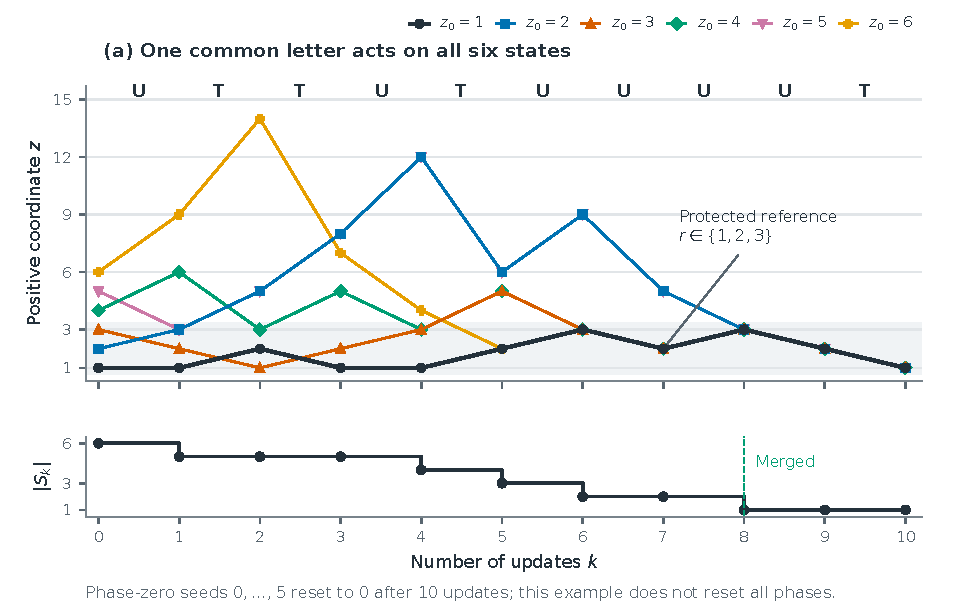
\includegraphics[width=\linewidth]{figures/synchronization.pdf}
\caption{Exact common control for \eqref{eq:small-reset-word}.
The six initial positive-coordinate values receive the same letter
at every time. Their tracks merge into the protected reference;
the distinct image count falls from six to one. The first merger
of the entire ensemble occurs at time eight, and the reference
returns to one at time ten.}
\label{fig:common-reset}
\end{figure}

Set $h_i=0$ for a $U$ letter and $h_i=1$ for a $T$ letter, with
the height read cyclically. For this example,
\begin{align}
 h&=(0,1,1,0,1,0,0,0,0,1),\nonumber\\
 d&=(1,0,-1,1,-1,0,0,0,1,-1),\label{eq:small-reset-forcing}\\
 b&=(0,1,2,0,1,1,2,1,2,2).\nonumber
\end{align}
Here $d_i=h_{i+1}-h_i$ and $b_i=r_i-1+h_i$.
Direct substitution gives $T(b_i)+d_i=b_{i+1}$, including the
last-to-first update. The three positive and three negative impulses
alternate, so the forcing is conservative and admissible. Its
primitive period is ten: a shorter period dividing ten would repeat
a shorter block either twice or five times, inconsistent with its
three positive impulses.

At phase zero the coordinate change is $z=n+1$. Thus the six
physical seeds $0,1,2,3,4,5$ correspond exactly to $S_0$ and all
satisfy
\begin{equation}\label{eq:small-physical-reset}
 F_{d,0}^{(10)}(n)=0\qquad(0\le n\le5).
\end{equation}
Repeating the word then follows the displayed response $b$.
The chosen launch phase is essential to this particular reset:
seed $5$ launched at phase one has value $3$ after ten updates,
whereas $b_1=1$. Thus \eqref{eq:small-physical-reset} does not
already give the one-period all-phase conclusion. The rotation
argument below supplies the additional condition needed to obtain
that stronger property for a suitable longer word.

The same construction gives periodic capture of any prescribed finite
set at one chosen phase. Start with
reference $1$, height zero, and the transformed values $n+1$ of the
specified nonnegative physical seeds. Apply an initial $U$, use
Lemma~\ref{lem:protected-merger}, and close the binary height word
back at zero. The period map sends every specified seed to zero.
During the reference response, the physical value is
$b=r-1+h\in B=\{0,1,2\}$: the only combination that would give
$b=3$ is $r=3,h=1$, which is forbidden by
\eqref{eq:reference-controller}. The next argument controls all
rotations and gives a logarithmic period bound.

\subsection{An explicit contraction estimate}

Sequential protected mergers prove existence, but during one merger
the other comparison values may grow. A period bound needs a quantity
that controls the entire current ensemble at once. A fractional power
is useful because it discounts the cost of an occasional growing step.
For example, strict concavity gives
\[
 \frac12\left[\left(\frac z2\right)^{1/4}
              +\left(\frac{3z}{2}\right)^{1/4}\right]
 <z^{1/4},
\]
whereas the corresponding average of the two values themselves is
exactly $z$. The reference constraint prevents us from choosing the
two letters with equal probability at every reference state. The
weights below compensate for that constraint.

For a finite set $S$ of \emph{distinct} positive integers containing
$r$, put
\begin{equation}\label{eq:sync-potential}
 P(r,S)=g_r\sum_{z\in S}z^{1/4},\qquad
 (g_1,g_2,g_3)=\left(\frac{19}{20},1,\frac{111}{100}\right).
\end{equation}
Choose the next letter with probabilities
\begin{equation}\label{eq:reference-probabilities}
 \mathbb P(T\mid r=1)=\frac{19}{39},\quad
 \mathbb P(T\mid r=2)=\frac{111}{206},\quad
 \mathbb P(T\mid r=3)=0.
\end{equation}
The same chosen letter acts on every member of $S$, and duplicate
images are discarded. Randomness is used only for an existence
argument about finite words.

There is a related random-map synchronization theorem of Yano and
Yasutomi: a finite irreducible aperiodic Markov chain admits a choice
of mapping law with synchronizing support
\cite{yano-yasutomi-2011}. In the present process, the maps
and their simultaneous action on the integer ensemble are prescribed.
Consequently, mixing of the finite reference chain alone does not
establish synchronization of the ensemble; its merger and drift
estimates must be proved for this common action.

The probabilities can be read directly from the reference weights.
At reference one, a $T$ step moves to reference two and a $U$ step
stays at one. Choosing $p_1=\mathbb P(T\mid r=1)$ to satisfy
\[
 p_1g_2=(1-p_1)g_1
\]
gives $p_1=g_1/(g_1+g_2)=19/39$. At reference two, the two
destinations are one and three. Balancing their contributions gives
\[
 p_2g_1=(1-p_2)g_3,
 \qquad p_2=\frac{g_3}{g_1+g_3}=\frac{111}{206}.
\]
Thus the coefficient of a shrinking branch equals the coefficient
of a growing branch, whichever letter provides it for a particular
input parity. At reference three the only letter is $U$, but its
destination has the smaller weight $g_2$. The chosen ratio
$g_3/g_2=111/100$ exceeds the fourth-root growth factor
$(3/2)^{1/4}$, allowing contraction even in that worst parity case.

Removing duplicate images is also part of the estimate. Once two
initial seeds share a current value, every remaining common letter
acts identically on them. They impose one remaining synchronization
condition, so the potential counts their common value once. In the
worked example, the six tracked labels eventually contribute just
one term to the potential, while the reference continues around its
small allowed state space.

\begin{lemma}[Fractional-power drift]\label{lem:protected-drift}
For this process,
\begin{equation}\label{eq:sync-drift}
 \mathbb E[P(r',S')\mid r,S]
 \le\frac{999}{1000}P(r,S)
    +\left(\frac{25P(r,S)}{19}\right)^{1/5}.
\end{equation}
In particular, with $K_0=16000$ and $\rho=1999/2000$,
\begin{equation}\label{eq:sync-geometric-drift}
 P(r,S)\ge K_0\quad\Longrightarrow\quad
 \mathbb E[P(r',S')\mid r,S]\le\rho P(r,S).
\end{equation}
\end{lemma}
\begin{proof}
Write $a=2^{-1/4}$ and $b=(3/2)^{1/4}$. For an even input the
two branch values are exactly $z/2$ and $3z/2$. For an odd input
they have an additional $1/2$. Ignoring this additive correction
temporarily, the expected gain of $g_{r'}z'^{1/4}$ relative to
$g_rz^{1/4}$ is bounded, for $r=1,2,3$, respectively by
\[
 \frac{20(a+b)}{39},\qquad
 \frac{10545(a+b)}{20600},\qquad
 \frac{100b}{111}.
\]
In the first two expressions the weighted probabilities of the two
letters are equal, so the bound is independent of the input parity.
The third is the larger of the two possible parity gains.
The rational inequalities $a<841/1000$ and $b<1107/1000$ follow
by taking fourth powers. They give the respective upper bounds
\[
 \frac{974}{975},\qquad
 \frac{1027083}{1030000},\qquad
 \frac{369}{370},
\]
each strictly below $999/1000$.

For $c\in\{1/2,3/2\}$, concavity gives
\[
 (cz+1/2)^{1/4}-(cz)^{1/4}
 \le\frac18(cz)^{-3/4}.
\]
Multiplication by $g_{r'}\le111/100$ bounds the correction by
$(111/800)2^{3/4}z^{-3/4}<z^{-3/4}/4$.
The last inequality follows from $8\cdot111^4<200^4$.
Discarding duplicate images can only reduce the potential.

If $m=|S|$ and its members are listed increasingly, the $j$th is
at least $j$. Comparison with integrals yields
\[
 \sum_{z\in S}z^{-3/4}
 \le\sum_{j=1}^{m}j^{-3/4}\le4m^{1/4},\qquad
 \sum_{z\in S}z^{1/4}\ge\sum_{j=1}^{m}j^{1/4}
 \ge\frac45m^{5/4}.
\]
Thus $P\ge(19/25)m^{5/4}$, and the total additive error is at
most $m^{1/4}\le(25P/19)^{1/5}$. This proves
\eqref{eq:sync-drift}. For $P\ge16000$,
$(25P/19)^{1/5}\le P/2000$: after taking fifth powers it is
enough that $19P^4\ge25\cdot2000^5$, which already holds at
$P=16000$ and is preserved as $P$ increases.
\end{proof}

\subsection{A uniform tail for synchronization}

The drift bounds the waiting time until the ensemble has small potential.
There Lemma~\ref{lem:protected-merger} gives a positive probability of
a reset in bounded time. After a failed trial the same drift bounds the
time to the next trial. This applies the drift and minorization method
\cite[Theorem~12]{rosenthal-1995} to the whole ensemble under a common
sequence of letters.

\begin{lemma}[Exponential synchronization tail]\label{lem:sync-tail}
Let $\tau$ be the first time the ensemble is the singleton containing
the reference. There are absolute constants $c,C_1>0$ such that
\begin{equation}\label{eq:sync-tail}
 \mathbb P_{r,S}(\tau>t)
 \le C_1\bigl(1+P(r,S)\bigr)e^{-ct}
 \qquad(t\in\N).
\end{equation}
\end{lemma}
\begin{proof}
Let $\mathcal C=\{(r,S):P(r,S)<K_0\}$. It is a finite set of
ensemble states: every member of such an $S$ is at most
$K=\lceil(320000/19)^4\rceil$. If $\sigma$ is the first entrance
time into $\mathcal C$, the killed version of
\eqref{eq:sync-geometric-drift} gives
\[
 \mathbb E[P(r_t,S_t)\mathbf1_{\{\sigma>t\}}]
 \le\rho^t P(r,S),\qquad
 \mathbb P(\sigma>t)\le\frac{P(r,S)}{K_0}\rho^t.
\]
For $0<\beta_0<-\log\rho$, the tail-sum identity for a
nonnegative integer-valued stopping time therefore gives
\begin{equation}\label{eq:entrance-moment}
 \mathbb E e^{\beta_0\sigma}
 \le1+a_0P(r,S),\qquad
 a_0=\frac{e^{\beta_0}-1}{K_0(1-\rho e^{\beta_0})}.
\end{equation}
In particular the entrance time is finite almost surely.

For each possible reference value, apply
Lemma~\ref{lem:protected-merger} to the entire finite interval
$\{1,\ldots,K\}$. Pad the resulting words by $U$ at reference
$1$ so that they have one common length $m_0$. Every positive
allowed letter probability in \eqref{eq:reference-probabilities}
is at least $95/206$. A trial of $m_0$ steps begun in
$\mathcal C$ therefore succeeds in synchronizing with conditional
probability at least
$\varepsilon=(95/206)^{m_0}>0$.

After any trial, define $D$ to be its length $m_0$ plus the
subsequent time needed to return to $\mathcal C$. This can be
defined whether or not the trial succeeds. The potential at the
end of a trial is uniformly bounded over initial states in
$\mathcal C$: each individual output is at most twice its input
at each step, the number of image points cannot increase, and the
three reference weights are bounded away from zero. Equation
\eqref{eq:entrance-moment} consequently implies
\[
 M_0:=\sup_{x\in\mathcal C}\mathbb E_x e^{\beta_0D}<\infty.
\]
Let $H$ be the event that synchronization has not occurred by the
end of the trial. Then $\mathbb P_x(H)\le1-\varepsilon$.
For $0<\theta<1$, H\"older's inequality gives
\[
 \mathbb E_x[e^{\theta\beta_0D}\mathbf1_H]
 \le M_0^\theta(1-\varepsilon)^{1-\theta}.
\]
Choose $\theta>0$ small enough that the right side is some
$\kappa<1$, and put $\beta=\theta\beta_0$.

Repeat the trial after each failed trial and return to
$\mathcal C$. The conditional failure bound ensures eventual
success almost surely. The strong Markov property and the preceding
weighted failure estimate bound the contribution of success on
trial $j$ to the exponential moment by
$e^{\beta m_0}\kappa^{j-1}$. Summing over $j\ge1$ and accounting
for the initial entrance time with
\eqref{eq:entrance-moment} gives
$\mathbb E e^{\beta\tau}\le C(1+P(r,S))$ for an absolute
$C$. Markov's inequality proves \eqref{eq:sync-tail}.
The argument uses conditional bounds and the strong Markov property;
it makes no independence assumption between different trials.
\end{proof}

For an interval ensemble $\{1,\ldots,N+2\}$, the initial potential
is at most $(111/100)(N+2)^{5/4}$. Consequently, for
$0<\varepsilon<1$, the probability of failure at a single chosen
phase is at most $\varepsilon$ whenever
\[
 t\ge\left\lceil\frac1c\left(\frac54\log(N+2)
                    +\log\frac1\varepsilon+C_4\right)\right\rceil
\]
for an absolute constant $C_4$.

\subsection{Closing the clock and treating every launch phase}

A closed reference path gives a periodic response. To reset the seeds
from every phase, each rotation of its label word must synchronize the
transformed seeds at that phase.

\begin{theorem}[Logarithmic all-phase synchronization]
\label{thm:all-phase-synchronization}
There exist absolute finite constants $C,C_0$ with the following
property. For every integer $N\ge1$ there is a nonzero conservative
admissible forcing word of odd prime primitive period $p$, with
\begin{equation}\label{eq:sync-period-order}
 \left\lceil\log_2(N+1)\right\rceil
 \le p\le C\log(N+2)+C_0,
\end{equation}
and a phase-indexed response $(b_i)_{i\bmod p}$ in $B=\{0,1,2\}$,
such that
\begin{equation}\label{eq:all-phase-reset}
 F_{d,i}^{(p)}(n)=b_i
 \quad\text{for every }i\text{ and every }1\le n\le N.
\end{equation}
Equation~\eqref{eq:all-phase-reset} also holds for $n=0$ at
every safe zero phase. The response contains zero, may be rotated
to have $b_0=0$, and has least scalar and augmented period $p$.
\end{theorem}
\begin{proof}
The reference chain specified by
\eqref{eq:reference-controller}--\eqref{eq:reference-probabilities}
has transition matrix and stationary distribution
\[
 P_{\rm ref}=
 \begin{pmatrix}
 20/39&19/39&0\\
 111/206&0&95/206\\
 0&1&0
 \end{pmatrix},\qquad
 \pi=\frac1{10048}(4329,3914,1805).
\]
Direct multiplication verifies $\pi P_{\rm ref}=\pi$.
There is a supported four-step path between every ordered pair
of reference states: pass through state $1$ along shortest
allowed paths, whose combined length is at most four, and fill
the remaining steps with its $U$ self-loop. Every positive
transition probability is greater than $9/20$. Hence every
entry of $P_{\rm ref}^4$ is greater than
$(9/20)^4>1/25$. Multiplying on the left by a stochastic matrix
preserves this entrywise lower bound, so
\begin{equation}\label{eq:reference-closure}
 \mathbb P_\pi(r_L=r_0)>1/25\qquad(L\ge4).
\end{equation}

A closed labeled reference path of length $L$ has probability
\[
 \pi(r_0)\prod_{j=0}^{L-1}p_{r_j}(w_j),
 \qquad w_j\in\{T,U\}.
\]
Cyclic rotation gives a bijection on the set of closed paths.
It preserves the product of transition factors and changes only
the initial stationary weight, whose ratio is at most
$\pi_{\max}/\pi_{\min}=4329/1805<5/2$.

Let $J_N=\{1,\ldots,N+2\}$. It contains every possible reference
and every required transformed physical seed at every height.
Its initial potential is at most
$(111/100)(N+2)^{5/4}$. Apply
Lemma~\ref{lem:sync-tail} to this ensemble from each initial
reference. For a given rotation, the probability mass of closed
paths whose rotated label word fails to synchronize $J_N$ is
bounded by $5/2$ times the unconditioned failure probability.
A union bound over the $L$ rotations therefore gives
\begin{equation}\label{eq:rotated-failure}
 \mathbb P_\pi\bigl(r_L=r_0\text{ and some rotation fails}\bigr)
 \le C_2 L(N+2)^{5/4}e^{-cL}
\end{equation}
for an absolute $C_2$.

For all $L$ above a sufficiently large constant multiple of
$\log(N+2)$ plus a sufficiently large constant, the right side
of \eqref{eq:rotated-failure} is below $1/25$. To see this
uniformly for all larger $L$, first use
$L\le C_3e^{cL/2}$ and then absorb $(N+2)^{5/4}$ into the
remaining exponential. Choose an integer threshold with these
properties and at least three. Bertrand's postulate supplies an
odd prime $p$ between it and twice it. This changes only the
absolute constants in the logarithmic upper bound.
By \eqref{eq:reference-closure}--\eqref{eq:rotated-failure}
there exists a closed length-$p$ reference path whose label word
and every rotation synchronize $J_N$ by time $p$.

This label word is nonconstant: powers of $T$ keep $1$ and $2$
distinct, whereas powers of $U$ keep $1$ separate from the cycle
$2\leftrightarrow3$. Since $p$ is prime, the label word is
primitive. Put $h_j=1$ for label $T$ and $h_j=0$ for label $U$,
and take cyclic differences $d_j=h_{j+1}-h_j$. By
Proposition~\ref{prop:height-conjugacy}, this is a nonzero
admissible conservative forcing with primitive period $p$.
The closed reference path gives
$b_j=r_j-1+h_j\in B$, and the conjugacy proves it is a
physical response. At phase $i$, each required physical seed
becomes a member of $J_N$. The rotated word sends that member
to $r_i$ after $p$ updates, proving
\eqref{eq:all-phase-reset}. If a merger occurs earlier, it
persists, so the equality at time $p$ is exact.

Conservation and cyclicity imply
\[
 0=\sum_{j=0}^{p-1}\bigl(T(b_j)-b_j\bigr)
   =\#\{j:b_j=1\}-\#\{j:b_j=2\}.
\]
As $p$ is odd, the response has a zero. Rotating to it gives
$b_0=0$. Any smaller scalar period would give a smaller forcing
period by $d_j=b_{j+1}-T(b_j)$, so the response is primitive.

Finally, at a height-zero phase the $N+1$ distinct safe inputs
$0,\ldots,N$ share one endpoint after $p$ steps. Each forced
step has at most two integer preimages of any value, one even
and at most one odd. Its $p$-fold composition has at most $2^p$
preimages. Hence $2^p\ge N+1$, giving the lower bound.
\end{proof}

The lower-bound argument applies to every nonzero word with the
stated one-period reset property, independently of the construction.
Thus the minimum possible primitive period has order
$\log(N+2)$. The proof gives finite absolute constants; it does
not provide practical optimal constants. Any finite seed set is
contained in an interval, so the theorem also synchronizes every
prescribed finite set at all launch phases.

\begin{corollary}[Many successful forcing families]
\label{cor:many-sync-families}
For each fixed $N$, every sufficiently large odd prime $p$ admits
at least
\[
 \frac1{50p}\left(\frac{206}{111}\right)^{\lfloor p/2\rfloor}
\]
distinct cyclic rotation classes of nonzero admissible forcing
words satisfying the all-phase conclusion of
Theorem~\ref{thm:all-phase-synchronization}.
\end{corollary}
\begin{proof}
For sufficiently large $p$, the closed-path mass is greater than
$1/25$ and the closed-path failure mass in
\eqref{eq:rotated-failure} is less than $1/50$. Good closed paths
therefore have total probability at least $1/50$. Put
$\eta=111/206$. At reference $1$ or $2$, each specified letter
has probability at most $\eta$. The only deterministic reference
state is $3$, which immediately moves to $2$. Thus every
length-$p$ path has at least $\lfloor p/2\rfloor$ transitions
from nondeterministic reference states. For each starting
reference, and hence also after averaging over $\pi$, a
specified label word has probability at most
$\eta^{\lfloor p/2\rfloor}$. There are at least
$\eta^{-\lfloor p/2\rfloor}/50$ successful label words.
All are primitive as in the theorem. Nonconstant binary height
words are uniquely determined by their cyclic differences, and
a rotation class contains at most $p$ rooted words. Dividing by
$p$ proves the claim.
\end{proof}

The word and response in Theorem~\ref{thm:all-phase-synchronization}
may depend on the prescribed interval. Capture for the fixed seven-step
word and ordinary Collatz convergence remain separate questions.
The logarithmic-period bound is an analytical result.

\section{Inverse basins in every arithmetic progression}\label{sec:inverse}

This section fixes the forcing $d=(1,0,-1)$, with phase zero immediately
before $+1$. Write $F(n)=F_{d,0}^{(3)}(n)$ for its return map. A target
$(v,i)$ is safe precisely when $v\ge0$ for $i=0$ and $v\ge1$ for $i=1,2$.
All predecessors below refer to this fixed forcing, with phase included.

\begin{theorem}[Inverse growth and arithmetic progressions]\label{thm:inverse-growth}
There is a number $\delta$, with $0.535<\delta<0.536$, such that the following
holds. For every safe target $(v,i)$, every modulus $M\ge1$, every residue
$a\bmod M$, and every launch phase $j$, there are constants $c>0$ and $X_0$
such that, for $X\ge X_0$, at least $cX^\delta$ positive integers $x\le X$
satisfy $x\equiv a\pmod M$ and their trajectories from phase $j$ reach
$(v,i)$. The constants may depend on the target, progression, and phase.
The exponent is defined exactly by
\begin{equation}\label{eq:inverse-exponent}
 \sum_{o=0}^{8}m_o(2^{24}/3^o)^{-\delta}=1,
 \qquad (m_0,\ldots,m_8)=(1,4,17,35,57,69,53,32,13).
\end{equation}
\end{theorem}

An exact finite certificate supplies the branches of a growing inverse
tree. A bounded-length selector sends its vertices into the required
progression with bounded size cost and multiplicity.

For ordinary Collatz, Monks proved that every positive orbit merges
with an orbit starting in any prescribed progression, possibly after
different numbers of steps \cite[Theorem~1.1]{monks-2006}.
Theorem~\ref{thm:inverse-growth} counts predecessors of a specified
target at a specified phase for the forced map.

\subsection{Elementary inverse branches and eligible targets}

The full three-step return has eight affine pieces.  In the table below,
the parity string is read in chronological order from the three inputs
to the shortcut map; it is not the binary expansion of the residue $r$.
Every row is valid for all integers $t\ge0$.
\begin{center}
\begin{tabular}{rrl|rrl}\toprule
$r$&parities&$F(8t+r)$&$r$&parities&$F(8t+r)$\\\midrule
0&010&$3t$&4&011&$9t+7$\\
1&111&$27t+7$&5&110&$9t+6$\\
2&001&$3t+1$&6&000&$t$\\
3&101&$9t+4$&7&100&$3t+2$\\\bottomrule
\end{tabular}
\end{center}
For example, the residue $r=3$ follows
\[
 8t+3\ \longmapsto\ 12t+6\ \longmapsto\ 6t+3
 \ \longmapsto\ 9t+4.
\]
The impulses are applied after the shortcut update at each arrow.
The slopes in the table range from $1$ to $27$ as functions of $t$.

Four convenient rows of the complete table give
\begin{equation}\label{eq:inverse-four}
 F(8t+6)=t,\quad F(8t)=3t,\quad
 F(8t+2)=3t+1,\quad F(8t+7)=3t+2.
\end{equation}
Consequently the following are inverse branches:
\[
 A(y)=8y+6,\quad B_0(y)=\frac{8y}{3},\quad
 B_1(y)=\frac{8y-2}{3},\quad B_2(y)=\frac{8y+5}{3}.
\]
Here $A$ is always applicable, and $B_r$ is applicable precisely when
$y\equiv r\pmod3$. For $y\ge2$ every applicable branch strictly increases
$y$ and its output $x$ satisfies $x+1\le8(y+1)$. Call a phase-zero value
\emph{eligible} if $y\ge2$ and $3\nmid y$.

Every phase-zero $u\ge0$ has an eligible predecessor two laps earlier.
Explicitly, choose
\begin{equation}\label{eq:eligible-attachment}
 y=\begin{cases}
 64u+54,&3\nmid u,\\
 64t+6,&u=3t,\ 3\nmid t,\\
 64t+16,&u=3t,\ 3\mid t.
 \end{cases}
\end{equation}
The formulas in \eqref{eq:inverse-four} prove $F^2(y)=u$ in each case;
$y\ge2$ and $3\nmid y$ are immediate. For a target $(v,1)$ or $(v,2)$,
the phase-zero values $2(v-1)$ and $4v-2$, respectively, reach that target
after one or two updates. These values are nonnegative on the safe domain.
Thus \eqref{eq:eligible-attachment} attaches every safe augmented target.

For instance, phase-zero targets $0,1,3,9$ have the eligible two-lap
predecessors $16,118,70,208$, respectively. Their exact returns are
\[
 16\mapsto6\mapsto0,\quad118\mapsto14\mapsto1,\quad
 70\mapsto8\mapsto3,\quad208\mapsto78\mapsto9.
\]
Each arrow in this display is one whole three-update lap. The third
case of \eqref{eq:eligible-attachment} matters even for target zero:
simply using $A^2(0)=54$ would give a parent divisible by three,
outside the eligible class used for the growing tree.

In the ordinary inverse graph a positive multiple of three has only
its iterated doublings as predecessors. The backtracing theorem of
Monks et al. assumes a target coprime to three
\cite[Theorem~4.1]{monks-et-al-2013}. Here
\eqref{eq:eligible-attachment} and the phase lifts cover every safe
target, including zero.

\subsection{The finite 24-step certificate}

Applegate and Lagarias enumerate ordinary inverse trees by depth,
residue class and odd-step count \cite[Sections~2--3]{applegate-lagarias-1995-i}.
Krasikov and Lagarias refine the estimates by residue-dependent
difference inequalities \cite[Theorems~2.2 and~6.1]{krasikov-lagarias}.
Here we enumerate forced branches, bound their sizes, and prove that
the branches counted in the inverse tree give distinct predecessors.

Put $S=2^{24}$. For an itinerary of 24 input parities with $o\le8$ odd
inputs, Proposition~\ref{prop:affine-parity} gives a unique initial residue
$r\bmod S$. Its inverse formula is
\begin{equation}\label{eq:inverse-offset}
 x=\frac{Sy+c}{3^o},\qquad c=3^or-SF^8(r).
\end{equation}
The row with no odd inputs is especially transparent: apply $A$ eight
times to obtain
\[
 A^8(y)=8^8y+6(1+8+\cdots+8^7)
       =2^{24}y+14{,}380{,}470.
\]
This verifies the first offset without an enumeration and explains why
24 literal updates correspond to eight returns of $F$.
Integrality restricts $y$ to one class modulo $3^o$. To count children
coprime to three, inspect its three lifts modulo $3^{o+1}$, retain those
with $3\nmid x$, and discard parents divisible by three. Distinct formulas
have distinct residues $r$, so their integer children are distinct.

\begin{lemma}[Certified branch minima]\label{lem:inverse-certificate}
For each $y\ge34$ with $3\nmid y$, and each $0\le o\le8$, there are at
least $m_o$ distinct children $x$ such that
\[
 F^8(x)=y,\qquad 3\nmid x,\qquad x>y,\qquad
 x+1\le(S/3^o)(y+1).
\]
\end{lemma}
\begin{proof}[Exact finite verification]
The complete enumeration and its output are
\path{certificates/inverse/certify_growth.py} and
\path{certificates/inverse/growth_certificate.json}. The algorithm enumerates
all $\sum_{o=0}^8\binom{24}{o}=1{,}271{,}626$ parity words with at most
eight odd inputs by composing inverse updates. For every formula it
recovers $r=c(3^o)^{-1}\bmod S$, rejects repeated $r$, independently replays
all 24 forward updates at $r$, and checks the odd count and offset.
It then counts the admissible children on every unit parent class modulo
$3^{o+1}$. The minima and offset extremes are as follows.
\begin{center}\small
\begin{tabular}{rrrrr}\toprule
$o$ & $m_o$ & Parity words & Minimum $c$ & Maximum $c$\\\midrule
0&1&1&14380470&14380470\\
1&4&24&1198370&15878434\\
2&17&276&-25765018&16440166\\
3&35&2024&-40594894&16650802\\
4&57&10626&-70928746&16729750\\
5&69&42504&-147774526&16759234\\
6&53&134596&-197825722&16769926\\
7&32&346104&-300203566&16772842\\
8&13&735471&-559561354&16770655\\\bottomrule
\end{tabular}
\end{center}
For each enumerated offset the checker verifies, using integers,
\[
 34(S-3^o)+c>0,\qquad c+3^o\le S.
\]
These inequalities imply strict growth and the size bound for every
$y\ge34$. A positive integral $x$ with residue $r\in[0,S)$ is $r+Sk$
with $k\ge0$, so the forward affine identity applies. Admissibility of the
forcing guarantees that its intermediate states are safe. The enumeration
and residue grids are finite and exhaust the indicated cases. This is a
computer-assisted finite lemma, not a Lean theorem in this release; the
hash in the output is an integrity aid, not the proof of its arithmetic.
\end{proof}

Set $L_o=S/3^o>1$. The left side of \eqref{eq:inverse-exponent} decreases
continuously from 281 to zero, establishing a unique positive root.
At exponent $1/2$ its value is
\[
 \frac{3049+1594\sqrt3}{4096}>\frac{4643}{4096}>1,
\]
so $\delta>1/2$ without numerical approximation. The reported interval
uses integer powers: with $G=10^9$, find $a_o$ such that
\[
 a_o^q S^p\le G^q3^{op}<(a_o+1)^q S^p.
\]
Then $a_o/G$ and $(a_o+1)/G$ bound $L_o^{-p/q}$ from below and strictly
from above. Weighted sums certify mass greater than one at $p/q=107/200$
and less than one at $67/125$. The value
$0.535422959115049\ldots$ is an approximation, not the definition.

Keeping the different size factors is essential to this exponent. If all
281 selected children were charged the common worst factor $S$, the
resulting exponent would be $\log(281)/\log(S)<1/2$, since
$281<\sqrt S=4096$. The certified gains come from the many children
with factors $S/3^o$ substantially smaller than $S$. Formula
\eqref{eq:inverse-exponent} retains those gains while still giving a
uniform argument at every eligible parent; it is not an estimate from
an average sampled trajectory.

\begin{lemma}[Weighted inverse counting]\label{lem:inverse-count}
For every eligible root $y\ge34$, its phase-zero backward orbit contains
at least $((X+1)/(S(y+1)))^\delta$ distinct values at most $X$, whenever
$X+1\ge S(y+1)$.
\end{lemma}
\begin{proof}
At every vertex retain exactly $m_o$ children of each type $o$, assigning
each edge weight $L_o^{-\delta}$. The outgoing weights sum to one.
Different paths of equal depth cannot collide, because $F^8$ determines
the parent uniquely. A collision of depths $a<b$ would, on applying $a$
forward blocks, identify the root with its own descendant of depth $b-a$.
Strict increase along inverse edges rules this out as well.

Write $W=(X+1)/(S(y+1))\ge1$. Stop a path when its product of edge factors
first reaches $W$. Since the smallest factor exceeds one, the stopping
tree has finite depth. Its stopped products lie between $W$ and $SW$;
the corresponding integers satisfy $x+1\le SW(y+1)=X+1$.
The weights of all stopped leaves sum to one, while each is at most
$W^{-\delta}$. Hence there are at least $W^\delta$ distinct leaves.
For $W=1$, stopping at the root gives the same assertion.
\end{proof}

\subsection{Ternary steering with uniform finite choices}

The modular translation and admissible backtracing strategy has direct
antecedents in Monks and Monks et al.
\cite{monks-2006,monks-et-al-2013}. The latter's Theorem~4.1 bounds the
number of \emph{odd inverse operations} needed to reach a progression,
independently of the target. Its convention $l(s)$ counts those operations,
whereas $\|s\|$ also counts the intervening even operations.
For the counting transfer here we need a finite selector with bounded
\emph{total physical length}, size cost, and multiplicity. The following
proofs establish these properties directly, including the integral domains
of the modular words; a bound on odd inverse count alone would not suffice.

\begin{lemma}[Ternary steering]\label{lem:ternary-steering}
For each $k\ge0$, every eligible target $q$ has an inverse predecessor
in every class modulo $3^k$, using a uniformly bounded number of branches
from $\{A,B_0,B_1,B_2\}$. The bound depends only on $k$.
There are also arbitrarily large such predecessors, if the length is
allowed to increase.
\end{lemma}
\begin{proof}
For $k=0$, the identity is a bounded-length choice, and the iterates
$A^h(q)$ supply arbitrarily large choices. Hence assume $k\ge1$.
The identities
\[
 A^{2h}(q)=\frac{64^h(7q+6)-6}{7},\qquad
 v_3(64^h-1)=2+v_3(h)\quad(h\ge1)
\]
show that the $A^2$ orbit of a unit $q$ modulo $3^k$ consists of all lifts
of its residue modulo 9, with period $3^{k-2}$ for $k\ge2$.
For completeness the valuation identity follows by writing $64=1+9\cdot7$:
if $3\nmid h$, the first binomial term has valuation two and the later
terms have larger valuation; replacing an exponent $h$ by $3h$ increases
the valuation by one, since $a^2+a+1$ has valuation one when $a\equiv1\pmod9$.
The differences of two orbit points therefore have valuation exactly
$2+v_3(h_1-h_2)$. There are $3^{k-2}$ distinct points, exactly the number
of lifts of one residue modulo 9.

If $q\equiv5$ or $7\pmod9$, one application of $A$ moves it to residue
$1$ or $8$, respectively. On residues $1,2,4,8\pmod9$, respectively use
$B_1,B_2,B_1,B_2$; their outputs are units congruent to $2,1,1,2\pmod3$.
Varying the input along its $A^2$ orbit modulo $3^{k+1}$ and then applying
that $B$ branch supplies all lifts of one unit class modulo three at
precision $3^k$. An optional $A$, which is invertible and swaps the two
unit classes modulo three, supplies the other class. This proves steering
to any unit residue at any precision, with a finite bound for fixed $k$.

For any residue $a\bmod3^k$, first steer to the unit
$z\equiv(3a+2)8^{-1}\pmod{3^{k+1}}$ and apply $B_1$.
Its output is $a\bmod3^k$. All inputs can be kept at least two; applicable
branches then increase them. To produce this $z$ at precision $3^{k+1}$,
use the $A^2$ orbit at precision $3^{k+2}$; its period is $3^k$.
An exponent $0\le h\le3^k-1$ therefore suffices. The initial adjustment
by $A$, the selected $B$ branch, the optional $A$, and the final $B_1$
cost at most four additional branches. Thus the total length is at most
$2(3^k-1)+4=2\cdot3^k+2$. Taking additional full periods instead
gives arbitrarily large outputs. This latter assertion does not have a
bounded length requirement.
\end{proof}

\begin{lemma}[Exact domains of positive inverse words]\label{lem:inverse-domains}
A word $w$ of $\ell$ branches from $\{B_0,B_1,B_2\}$ has affine form
$B_w(y)=(8^\ell y+C_w)/3^\ell$. There is exactly one input residue modulo
$3^\ell$ on which every intermediate branch is integral and applicable.
Given any input residue $a\bmod3^k$, a word of $k$ letters can be chosen
whose domain is exactly that residue.
\end{lemma}
\begin{proof}
Composition proves the affine form. Final integrality gives a unique
residue, since 8 is invertible modulo $3^\ell$. Reducing that congruence
modulo $3^t$ gives the integrality condition for the first $t$ operations:
in the remaining affine composition its prefix numerator is multiplied
by a power of 8 and all later contributions have a factor $3^t$.
Thus all prefixes are integral. At each step exactly one of the three
formulas has integral value on a given residue modulo three; integrality
therefore is the stated branch condition. To get a word for $a$, start
with a sufficiently large positive representative of $a$ and choose its
applicable branch successively $k$ times. The unique domain contains $a$.
\end{proof}

For a concrete instance of the domain lemma, apply $B_2$ and then $B_1$.
The composed formula is
\[
 B_1(B_2(y))=\frac{64y+34}{9},\qquad y\equiv2\pmod9.
\]
Targets $y=2$ and $y=11$ give the legal inverse histories
$2\mapsto7\mapsto18$ and $11\mapsto31\mapsto82$.
Indeed $F^2(18)=2$ and $F^2(82)=11$. At $y=5$ the first branch gives
$B_2(5)=15$. The second requires residue $1\pmod3$, and the composed fraction
is nonintegral.

\begin{lemma}[Simultaneous odd-modulus steering]\label{lem:odd-steering}
Let $k\ge0$, $m\ge1$, and $\gcd(m,6)=1$. Every eligible target has a
predecessor in any specified class modulo $3^km$. For fixed $k,m$, the
choice can be made from a finite list of inverse words of bounded length.
Arbitrarily large choices also exist when length is unrestricted.
\end{lemma}
\begin{proof}
For $m=1$ use Lemma~\ref{lem:ternary-steering}. Otherwise all $B_r$ act as
permutations modulo $m$ with common linear coefficient $8/3$. Let $e$ be
the multiplicative order of $8/3$ modulo $m$, and put $Q=me$. Raising a
$B_r$ to power $e$ gives a translation, and raising a translation to power
$m$ gives the identity. Hence $B_r^Q$ is the identity modulo $m$, and its
inverse is represented by the positive word $B_r^{Q-1}$.

Modulo $m$ one has $B_1^{-1}B_0(y)=y+1/4$. Four repetitions give
translation by one. Replacing every inverse letter by $Q-1$ positive
copies produces a positive word $P$ of length $4Q$ representing $y+1$.
Let $w_0$ be the $k$-letter word from Lemma~\ref{lem:inverse-domains}
whose domain is the prescribed class $a\bmod3^k$. In application order
concatenate $w_0$, a positive representative of $w_0^{-1}$ modulo $m$,
and $P$, obtaining a word $V$ of length $\ell=Q(k+4)$.
It acts as translation by one modulo $m$, and every admissible use of it
starts in class $a\bmod3^k$.

The word $V^m$ has a unique admissibility class modulo $3^{m\ell}$.
Use ternary steering to obtain a predecessor $z\ge2$ of the original
target in that class. All letters of $V^m$ are then applicable.
The block boundaries $z,V(z),\ldots,V^{m-1}(z)$ start admissible copies
of $V$, so they all lie in class $a\bmod3^k$ and run through every
residue modulo $m$. Select the required one. For fixed moduli, the finite
ternary choice and at most $m-1$ copies of $V$ give a uniform length bound.
Using arbitrarily large ternary choices proves the separate unbounded-size
assertion. This domain argument is necessary: the modular permutation
calculation alone does not license arbitrary integer applications of $B_r$.
\end{proof}

\subsection{Binary digits, phases, and preservation of the exponent}

\begin{lemma}[Finite selector]\label{lem:finite-selector}
Fix a progression $a\bmod M$ and a launch phase $j$. There are constants
$D,C$ and finitely many rational affine formulas such that every eligible
phase-zero $y$ has an integer predecessor $x>0$ in that progression, at
phase $j$, given by one of these formulas on its exact admissibility
domain, reaching $y$ within $D$ physical updates and satisfying
$x+1\le C(y+1)$.
\end{lemma}
\begin{proof}
Write $M=2^\alpha3^bm$ with $\gcd(m,6)=1$. Choose a positive
representative $x_0$ of the progression. Choose $K\ge\alpha$ such that
launch phase $j$ reaches phase
zero in $K$ updates. Let its endpoint be $A_0$ and let $o$ count the odd
inputs in these $K$ updates. By the finite parity formula, for $t\ge0$,
\begin{equation}\label{eq:prefix-lift}
 x_0+2^K3^bmt\ \longmapsto\ A_0+3^{o+b}mt.
\end{equation}
The difference at each odd step is multiplied by $3/2$, at each even
step by $1/2$, and all impulses cancel from the difference. All sources
in \eqref{eq:prefix-lift} lie in the requested progression.

Choose a fixed $R$ such that $A^R(2)\ge\max(A_0,2)$, and first replace
$y$ by $A^R(y)$, still an eligible predecessor of $y$.
Lemma~\ref{lem:odd-steering} supplies a predecessor $z$ in class
$A_0\bmod3^{o+b}m$ with uniformly bounded inverse length. Branches grow
on inputs at least two, so $z\ge A_0$. Solving \eqref{eq:prefix-lift}
for $t$ gives a nonnegative integer and a positive $x$ in the progression.
The finite alphabet and length bound give finitely many affine formulas.
Their positive slopes and constant offsets give a common size constant
$C$ on $y\ge2$. The total physical length, including the fixed prefix
and padding, has a common bound $D$.
\end{proof}

\begin{proof}[Proof of Theorem~\ref{thm:inverse-growth}]
Attach an eligible phase-zero predecessor to the target using
\eqref{eq:eligible-attachment} and the phase lifts. If necessary, two
applications of $A$ put it above 34, since $A^2(2)=182$. Apply
Lemma~\ref{lem:inverse-count} to this root. Its at least $c_0Y^\delta$
eligible tree vertices below $Y$ each admit a selector predecessor
$x\le C(Y+1)-1$. A fixed output $x$ can be assigned to at most $D+1$
different tree vertices: they must appear among its first $D+1$ augmented
forward states. Thus there are at least $c_0Y^\delta/(D+1)$ distinct
outputs. Replacing $Y$ by $(X+1)/C-1$ proves the required lower bound
for all sufficiently large $X$.
\end{proof}

\begin{corollary}[A conditional route from exceptional-set bounds]
\label{cor:exceptional-set}
For this three-step forcing, fix a finite catalog of safe cycles and let
$E_j$ be the positive seeds at phase $j$ whose orbits never enter the
catalog. If one such exceptional safe trajectory exists, every progression
at every launch phase contains at least $cX^\delta$ exceptional seeds
below $X$ for all sufficiently large $X$. Consequently, a bound
$\#(E_j\cap\{x\le X:x\equiv a\pmod M\})=o(X^\delta)$ in even one
whole progression implies global capture. A bound $O(X^{1/2})$ suffices.
\end{corollary}
\begin{proof}
Every predecessor of an exceptional target is exceptional, since entry
into a cycle is forward invariant. Apply Theorem~\ref{thm:inverse-growth}
to that target. The claimed upper bound would contradict the resulting
lower bound. Since $\delta>1/2$, $O(X^{1/2})=o(X^\delta)$.
\end{proof}

The required exceptional-set upper bound remains open. Disjoint basins
can both have the stated inverse growth. Krasikov and Lagarias obtain
larger lower exponents for ordinary Collatz \cite{krasikov-lagarias}.

Tao's ordinary-map theorem concerns minima below any prescribed threshold
tending to infinity, for a set of logarithmic density one
\cite[Theorem~1.3 and Remark~1.4]{tao}. It supplies no exceptional-set upper
bound of the form required by Corollary~\ref{cor:exceptional-set} for this
forced map. Even natural-density-one capture would give only $o(X)$
exceptions, which does not imply $o(X^\delta)$ when $\delta<1$.

\section{Integer basins and a cosine continuation}
\label{sec:geometry}

For $(1,0,-1)$, integer capture means eventual entry into a phased
cycle. For its cosine continuation, a complex start belongs to the basin
if its iterates converge to the cycle at matching phases.

\subsection{Integer cycles and the phase-zero return}

Fix $d=(1,0,-1)$ and let
\[
 \Phi(n,i)=(T(n)+d_i,i+1\bmod3),\qquad
 F(n)=F_{d,0}^{(3)}(n).
\]
The safe integer state space consists of $n\ge0$ at phase zero and
$n\ge1$ at phases one and two. The following cycles are different
closed paths in that space.

\begin{proposition}[Exact nonnegative cycles]
\label{prop:geometry-cycles}
The augmented map has the cycles
\begin{align*}
 \Gamma_3:\quad &(0,0)\to(1,1)\to(2,2)\to(0,0),\\
 \Gamma_9:\quad &(1,0)\to(3,1)\to(5,2)\to(7,0)
 \to(12,1)\to(6,2)\\
 &\hspace{33mm}\to(2,0)\to(2,1)\to(1,2)\to(1,0).
\end{align*}
Their least augmented and scalar periods are respectively three and
nine. At phase zero, the first is the fixed point $F(0)=0$ and the
second is the three-cycle $1\mapsto7\mapsto2\mapsto1$.
\end{proposition}
\begin{proof}
Substitution in the signed shortcut rule verifies every arrow, including
$T(0)+1=1$ and $T(2)-1=0$. Within either displayed loop the augmented
states are distinct, so the first repeated augmented state occurs at
the stated length. The forcing is primitive of period three. The
period relation proved in Section~\ref{sec:foundations} shows that a
scalar cycle must already have period divisible by three. The three
different phase-zero values on $\Gamma_9$ rule out scalar period three.
\end{proof}

\begin{figure}[htbp]
 \centering
 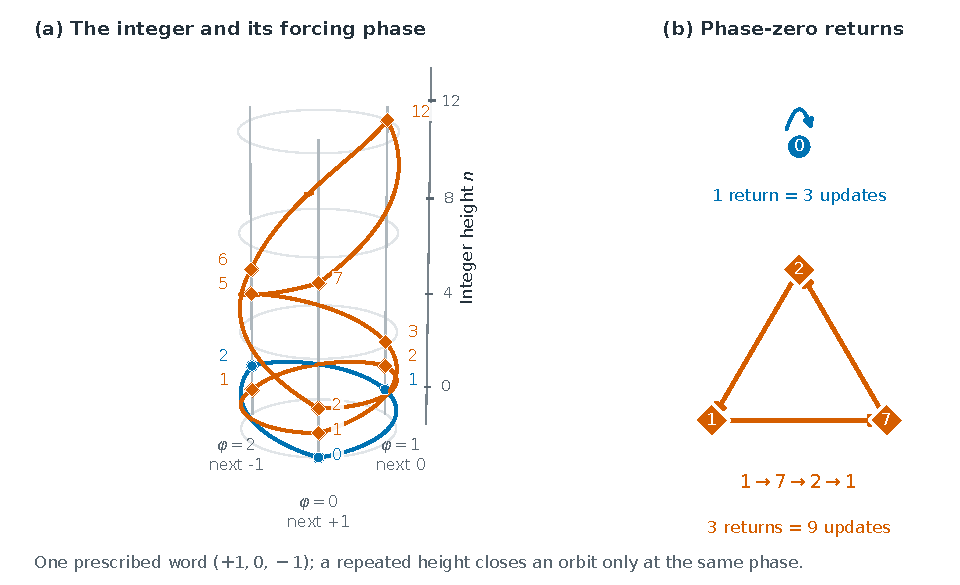
\includegraphics[width=.94\linewidth]{figures/phase_cycles.pdf}
 \caption{Exact integer cycles with the forcing phase retained. Sampling
 once every three physical updates gives a fixed point and a three-cycle
 of the phase-zero return. Equal scalar heights on different phase
 sheets are distinct states.}
 \label{fig:phase-cycles}
\end{figure}

At phase zero the eight return branches of Section~\ref{sec:inverse}
are, for $q\ge0$,

\begin{equation}\label{eq:geometry-return-table}
 F(8q+r)=3^{o_r}q+c_r,
 \qquad
 \begin{array}{c|rrrrrrrr}
 r&0&1&2&3&4&5&6&7\\\hline
 o_r&1&3&1&2&2&2&0&1\\
 c_r&0&7&1&4&7&6&0&2
 \end{array}
\end{equation}
At each of the three updates the coefficient of $q$ is even, so the
constant term fixes the parity on the entire ray.
\path{certificates/geometry/discrete.py} propagates both coefficients
and checks the cycles.

\begin{figure}[htbp]
 \centering
 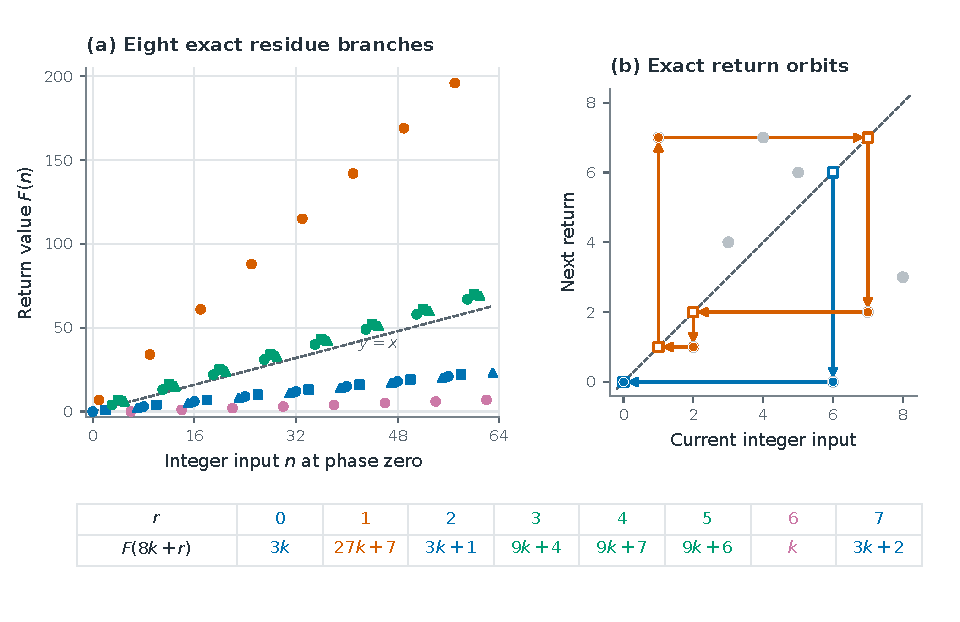
\includegraphics[width=.94\linewidth]{figures/integer_return.pdf}
 \caption{The eight residue-affine branches of the integer return and
 an exact return orbit. An affine branch applies only to its indicated
 residue class; a connecting line is a plotting aid, not a new
 continuous definition of the integer map.}
 \label{fig:integer-return}
\end{figure}

Let $\mathcal B_{3,i}$ and $\mathcal B_{9,i}$ denote the safe integer
seeds at phase $i$ eventually entering $\Gamma_3$ and $\Gamma_9$.
The basins are disjoint by determinism. Other cycles and unbounded safe
orbits remain possible.

\subsection{Basin interlacing and binary zooms}

\begin{corollary}[Both basins in every arithmetic neighborhood]
\label{cor:geometry-interlacing}
For every launch phase $i$, modulus $M\ge1$, and residue $a\bmod M$,
both $\mathcal B_{3,i}$ and $\mathcal B_{9,i}$ contain at least
$cX^\delta$ positive seeds at most $X$ in that residue class, for all
sufficiently large $X$. The positive constant and threshold may differ
between the two basins and may depend on the phase and progression;
$\delta$ is the exponent in Theorem~\ref{thm:inverse-growth}.
\end{corollary}
\begin{proof}
Apply Theorem~\ref{thm:inverse-growth} first to the safe augmented
target $(0,0)$ and then to $(1,0)$, with the prescribed launch phase
and progression. A predecessor of the first target belongs to
$\mathcal B_{3,i}$; a predecessor of the second belongs to
$\mathcal B_{9,i}$. The targets lie on the distinct cycles just proved.
\end{proof}

In particular, no finite number of low binary digits determines the
basin. By Proposition~\ref{prop:affine-parity}, a specified finite
input-parity word at a fixed phase is one residue class modulo a power
of two. The corollary gives arbitrarily large seeds in \emph{both}
basins with that same parity prefix. Even prescribing additional
ternary digits or any other fixed modulus does not change this fact.
For example, $9$ and $25$ are both $9\bmod16$, but their phase-zero
return orbits reach different cycles. The first follows
\[
 9\to34\to13\to15\to5\to6\to0,
\]
whereas the second eventually reaches $1\to7\to2\to1$.
The atlas interleaves the binary digits of each seed into two screen
coordinates. Each successive quadrant fixes two more low bits. A seed
receives a basin color when its integer trajectory reaches the cycle.
The remaining seeds stay unclassified at the iteration limit.

\begin{figure}[htbp]
 \centering
 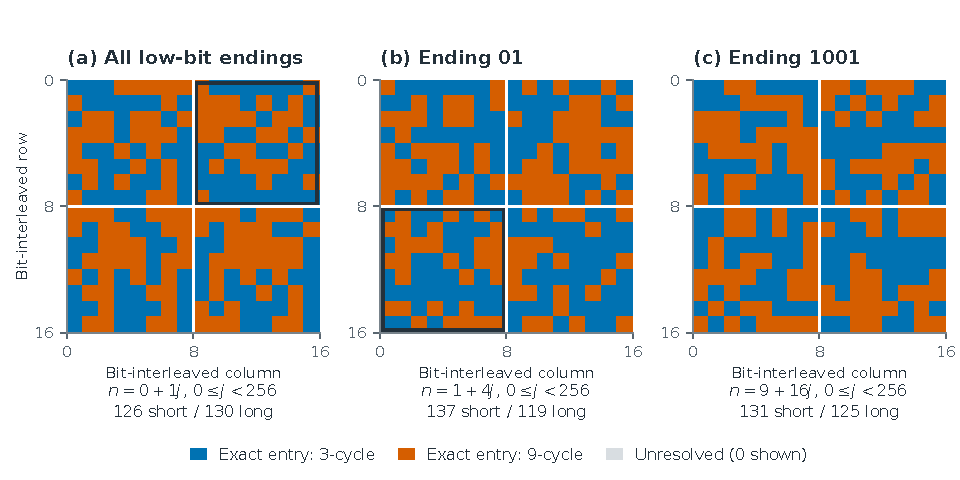
\includegraphics[width=.94\linewidth]{figures/binary_basins.pdf}
 \caption{An integer basin atlas arranged by low binary digits.
 Each colored sample is a particular integer with a replayed cycle
 destination. Corollary~\ref{cor:geometry-interlacing}, rather than the
 pixel count, proves that both basins occur in every fixed binary
 residue class at arbitrarily large heights.}
 \label{fig:binary-basins}
\end{figure}

One nested family of tiles is an \emph{exact copy} of the entire
integer dynamics, including any behavior that has not been classified.

\begin{proposition}[Exact binary zoom]\label{prop:binary-zoom}
Put $E(y)=8y+6$ and
$c_k=6(8^k-1)/7$. For every $k\ge0$ and $y\ge0$,
\begin{equation}\label{eq:binary-zoom}
 E^k(y)=8^ky+c_k,\qquad F^k(E^k(y))=y.
\end{equation}
Every nonnegative integer congruent to $c_k\pmod{8^k}$ has this
form with a unique $y\ge0$. Its first $3k$ physical input parities
are even. In particular, it belongs to a cycle basin at phase zero
if and only if its quotient seed $y$ belongs to that basin.
\end{proposition}
\begin{proof}
One literal lap is
\[
 8y+6\ \longmapsto\ 4y+4\ \longmapsto\ 2y+2
 \ \longmapsto\ y.
\]
All three input values are even, and the final value is at the initial
phase. Iteration proves the return and parity assertions. The affine
formula follows either by induction or by summing a geometric series.
Since $0\le c_k<8^k$, division with remainder proves the assertion
about every nonnegative member of the residue class. Appending a
finite initial path to a trajectory changes neither its eventual
cycle nor its failure to enter a specified cycle.
\end{proof}

Appending the three low bits $110$ is precisely the operation $E$.
For instance, $E^3(0)=438$ and $E^3(1)=950$ share nine low bits and
nine even inputs before reaching different cycles.
The all-depth identity is also certified by
\path{lean/inverse/Collatz/BinaryZoom.lean}; the figure is only a finite
view of that identity.

In the $2$-adic metric $|u-v|_2=2^{-v_2(u-v)}$, the two basins are
dense in the space of $2$-adic integers: each residue neighborhood
contains members of each basin by Corollary~\ref{cor:geometry-interlacing}.
The zoom identity gives the concrete common accumulation point
\[
 E^k(y)+\frac67=8^k\left(y+\frac67\right),
 \qquad E^k(y)\longrightarrow-\frac67\quad\text{in }\mathbb Z_2.
\]
For fixed $y\ge0$, these seeds tend to $+\infty$ in the real metric.
Membership in either basin fails to be ultimately periodic because
every residue class of any proposed period contains arbitrarily large
seeds from both basins. Their natural densities remain undetermined.

\subsection{The cosine continuation}

Between integer inputs we use the entire function

\begin{equation}\label{eq:cosine-extension}
 C(w)=w+\frac14-\left(\frac w2+\frac14\right)\cos(\pi w),
 \qquad w\in\mathbb C.
\end{equation}
On the real line this is Chamberland's interpolation
\cite{chamberland-1996,chamberland-survey}. At integers,
$\cos(\pi n)=(-1)^n$ gives $C(n)=T(n)$. The phased update is
$\Phi_C(w,i)=(C(w)+d_i,i+1\bmod3)$, with phase-zero return

\begin{equation}\label{eq:complex-return}
 R(w)=C\bigl(C(C(w)+1)\bigr)-1.
\end{equation}
Thus $R(n)=F(n)$ at every integer.

This interpolation is part of the model. For example,
$C(w)+\lambda\sin^2(\pi w)$ has the same values and first derivatives
at every integer for every fixed $\lambda$, while its values away from
the integers are different. Thus even exact knowledge of all integer
orbits and their linear multipliers does not specify the off-integer
function. Results about the following disks and separator refer to
\eqref{eq:cosine-extension} with the stated forcing.

Dumont and Reiter compare this cosine interpolation with a distinct
\emph{3-power} extension that agrees at integers and has the same
integer derivatives, while differing between the integers
\cite[Sections~1--2]{dumont-reiter-2003}.
Letherman, Schleicher and Wood construct selected entire extensions
for which all integers belong to the Fatou set and a noneventually
periodic integer would belong to a wandering domain
\cite{letherman-schleicher-wood-1999}.
Their family does not contain the cosine interpolation, as noted
explicitly by Dumont and Reiter \cite[Section~1]{dumont-reiter-2003}.
Those global Fatou-set conclusions therefore do not follow for $R$
from agreement with integer Collatz values.

The derivatives needed below are
\begin{align}
 C'(w)&=1-\tfrac12\cos(\pi w)
       +\pi(w/2+1/4)\sin(\pi w),\label{eq:cosine-derivative}\\
 C''(w)&=\pi\sin(\pi w)+\pi^2(w/2+1/4)\cos(\pi w).
 \label{eq:cosine-second}
\end{align}
In particular, $C'(n)=1/2$ at even integers and $3/2$ at odd
integers. An impulse is a translation, so it contributes derivative
one. A cycle with $L$ physical updates and $o$ odd integer inputs
therefore has multiplier $3^o/2^L$ over a \emph{complete} cycle.
For $\Gamma_3$ this is $3/8$; for $\Gamma_9$ it is $243/512$.
The one-lap derivative at the phase-zero point $1$ of $\Gamma_9$
is instead $27/8>1$. The following two laps have derivatives $3/8$
and $3/8$, and their product gives the contracting nine-step
multiplier. A growing portion of a return cycle is compatible with
attraction of the whole cycle.

\begin{proposition}[Attraction of admissible integer cycles]
\label{prop:integer-cycle-attraction}
Every nonnegative integer cycle of a nonzero conservative admissible
word is locally attracting under the phasewise cosine interpolation.
\end{proposition}
\begin{proof}
Every nonnegative periodic orbit lies in the safe domain: zero at a
height-one phase would remain zero until the next negative impulse
and then become negative. Use the binary height from
Proposition~\ref{prop:height-conjugacy} and write
$z_j=n_j+1-h_j>0$ along the cycle. Let
$e_j=n_j\bmod2$ and $\epsilon_j=z_j\bmod2$. The two height cases give
the same exact identity
\[
 2z_{j+1}=3^{e_j}z_j+\epsilon_j.
\]
Divide by $z_j$ and multiply around the cycle. If its length is $L$
and $o=\sum e_j$, then
\[
 2^L=\prod_{j=0}^{L-1}
       \left(3^{e_j}+\frac{\epsilon_j}{z_j}\right)
 \ge3^o.
\]
Equality is impossible because $L\ge1$ and powers of two and three
are different. Hence $3^o/2^L<1$. By the chain rule this is the
derivative of the full complex return at the periodic point. Continuity
of that derivative gives a small closed disk on which its modulus is
uniformly below one. Since the center is fixed, integration on line
segments makes that return a contraction mapping the disk into itself.
All points in the disk converge to the periodic point; the intermediate
phase maps give convergence along the entire cycle.
\end{proof}

For the unforced cosine map, positive integer-cycle attraction is
Chamberland's Theorem~3.3 \cite{chamberland-1996}.
Proposition~\ref{prop:integer-cycle-attraction} is also an application
of the generalized attraction theorem of Sindee, Sa Ngiamsunthorn
and Sriwongsa \cite[Theorem~3.3]{sindee-2024}, after the following
reduction. Fix a phase and a complete forcing period $p$. Each
residue class modulo $2^p$ fixes the $p$ physical input parities.
In the positive coordinate $z=n+1-h_i$, repeated use of the
one-step identity in the proof gives a return branch
\[
 G(z)=\frac{3^{o_r}z+b_r}{2^p},\qquad b_r\ge0,
 \qquad z\equiv r\pmod{2^p}.
\]
In their notation, the denominator is $d=2^p$, the slope numerator
is $m_r=3^{o_r}$, and the signed offset is $r_r=-b_r\le0$.
Integrality of the branch gives $r_r\equiv r m_r\pmod d$.
In particular, $\gcd(m_r,d)=1$, as their relatively-prime-type
hypothesis requires. Their interpolating indicators have zero
derivative at integers \cite[Lemma~2.2]{sindee-2024}, so their
extension has derivative $3^{o_r}/2^p$ there. If $R_i$ denotes the
physical cosine return at phase $i$, its positive-coordinate conjugate
is $\widehat R_i(z)=R_i(z-1+h_i)+1-h_i$. This conjugate agrees
with $G$ at integers and has the same derivative by the chain rule. Its integer-cycle
multiplier therefore agrees with theirs, and their strict bound
gives local complex attraction by the contraction argument above.
This transfers the integer multipliers without identifying the
two functions away from the integers.

The arithmetic return inequality is also formalized as
\path{Collatz.Physical.cycle_multiplier_lt_one} in
\path{lean/inverse/Collatz/CycleMultiplier.lean}. The subsequent
complex derivative and contraction arguments remain analytical.

\subsection{Uniform capture disks around the integer cycles}

The entire continuation also contains the signed cycle
$(-1,0)\to(0,1)\to(0,2)\to(-1,0)$, with multiplier $3/8$.
It is outside the safe nonnegative integer state space, but it is a
legitimate attractor to include in a complex-plane plot.

\begin{proposition}[Explicit integer capture disks]
\label{prop:integer-capture-disks}
A complex point within $10^{-6}$ of any center of these three
integer cycles, at the center's matching phase, converges to that
cycle. A valid complete-cycle error factor is
\begin{align*}
 q_3&=\frac{105633}{262144}<1
 &&\text{for either three-cycle},\\
 q_9&=\frac{10183907144921697}{18014398509481984}<1
 &&\text{for the nine-cycle}.
\end{align*}
\end{proposition}
\begin{proof}
For an integer center $n$, put $a_n=1-(-1)^n/2$. Direct expansion gives
\[
 C(n+w)-C(n)-a_nw
 =(-1)^n(n/2+1/4+w/2)\bigl(1-\cos(\pi w)\bigr).
\]
The power series implies
$|1-\cos u|\le |u|^2e^{|u|}/2$. For $|n|\le12$ and
$|w|\le r_*=1/4096$, using $e^t\le(1-t)^{-1}$ for $0\le t<1$,
the coefficient of $|w|^2$ is at most
\[
 \frac{(25/4+r_*/2)\pi^2}{2(1-\pi r_*)}<64.
\]
The final inequality is an exact rational comparison with the certified
upper bound on $\pi$ described below. Thus one physical step multiplies
the error by at most $a_n+64r_*=a_n+1/64$.

The even factor is $33/64<1$ and the odd factor is $97/64<2$.
At most five odd centers occur in any partial traversal of a displayed
cycle. Starting with error at most $10^{-6}$ therefore keeps every
intermediate error below $32\cdot10^{-6}<r_*$. This justifies using
the estimate at the next step, inductively. Multiplying all factors
around each cycle gives the displayed $q_3$ and $q_9$. After a complete
cycle the error is smaller, so the argument repeats and tends
geometrically to zero. The impulse cancels when the perturbed point
and its cycle center are compared.
\end{proof}

\subsection{Two certified noninteger attractors}

For the chosen continuation there are also positive noninteger cycles
of periods three and nine. The decimal numbers below are \emph{exact
rational centers of enclosing disks}, not asserted exact orbit points.
Let $D_i=\{w:|w-c_i|\le r_i\}$, and express the radii in units of
$10^{-6}$. In each table, rows advance in physical time and the last
disk maps back into the first.

\begin{center}\small
\begin{tabular}{rrlrr}\toprule
Step&Phase&Center $c_i$&Radius units&Derivative bound $L_i$\\\midrule
0&0&1.045673204662&100&1.14876\\
1&1&3.060567710576&130&0.43587\\
2&2&5.058720096962&60&0.11196\\
3&0&7.040922064888&10&0.02317\\
4&1&12.030267292222&1.1&2.37108\\
5&2&6.043435831841&3&1.90298\\
6&0&2.052131519289&6&1.16042\\
7&1&2.043141227448&8&1.04448\\
8&2&1.033231466989&10&1.24641\\\midrule
0&0&0.177527602643&10&1.13910\\
1&1&1.140098603174&11.8&0.35484\\
2&2&2.131993200359&4.4&2.20812\\\bottomrule
\end{tabular}
\end{center}

\begin{proposition}[Noninteger trapping cycles]
\label{prop:noninteger-traps}
Each table encloses one real, positive, noninteger periodic orbit.
Their least scalar and augmented periods are nine and three,
respectively. Every point in a listed disk converges to the
corresponding orbit at matching phases. Complete-cycle Lipschitz
bounds are at most $0.008854$ and $0.892519$, respectively. The
signed multipliers of the actual real cycles lie in
$[0.008141,0.008854]$ and $[0.891683,0.892509]$.
\end{proposition}
\begin{proof}
For a real center $c$ and radius $r$ with $\pi r<1$, the complex
trigonometric bounds on its disk are
\[
 |\sin(\pi w)|,|\cos(\pi w)|\le e^{\pi r}
 \le\frac1{1-\pi r}.
\]
Equation~\eqref{eq:cosine-second} therefore gives the uniform bound
\[
 M(c,r)=\frac{\pi+(|c/2+1/4|+r/2)\pi^2}{1-\pi r}
 \quad\text{on }|C''(w)|.
\]
If a rational interval encloses $C'(c)$, then its maximal absolute
endpoint plus $M(c,r)r$ bounds $|C'|$ on the disk. Round this quantity
up to the five-decimal rational $L_i$ in the table. The program
\path{certificates/geometry/attracting_disks.py} verifies
\begin{equation}\label{eq:disk-inclusion}
 |C(c_i)+d_i-c_{i+1}|\le10^{-12},\qquad
 10^{-12}+L_i r_i<r_{i+1},\qquad \prod_iL_i<1.
\end{equation}
The smallest inclusion slacks in the two tables are exactly at least
$291059/10^{12}$ and $212887/10^{12}$. Thus each phase map sends its
closed disk strictly inside the next disk. The complete composition
is a contraction of the initial disk into itself. The Banach fixed
point theorem gives a unique periodic point there and convergence of
every point of that disk. The same reasoning applies at every cyclic
starting row.

Complex conjugation commutes with the maps and preserves every disk,
so uniqueness makes the periodic points real. Every disk lies in the
positive half-plane and avoids the integers. The three disks of each
fixed phase in the nine-step table are disjoint, ruling out a
three-step augmented period. A three-step forcing has no shorter
augmented period. The identity $d_i=w_{i+1}-C(w_i)$ shows that a
scalar period is also a forcing period, so the same phase argument
rules out a smaller scalar period. Finally, at each real orbit point
$C'$ lies in its center-derivative interval enlarged by
$[-M(c_i,r_i)r_i,M(c_i,r_i)r_i]$. Multiplying these signed intervals,
with outward rounding, gives the stated multiplier enclosures.
\end{proof}

The checker bounds $\pi$ using Machin's identity
\[
 \pi=16\arctan(1/5)-4\arctan(1/239)
\]
and 24 terms of each alternating arctangent series, giving
\[
 3.14159265358979323846<\pi<3.14159265358979323847.
\]
Reducing $c$ by its nearest integer makes
the absolute real trigonometric argument less than two. Taylor
polynomials of degrees fourteen for cosine and fifteen for sine,
with the next-degree real remainder bounds, enclose the center values
and derivatives. All signs, endpoint products, radius inclusions,
and outward roundings use integer fractions. The displayed decimal
roundings are therefore part of exact rational comparisons.

Dumont and Reiter plot escape times, stopping times, and basins for
complex Collatz interpolations \cite{dumont-reiter-2001}. Here the
numerical plot uses the forced return \eqref{eq:complex-return}.

\begin{figure}[htbp]
 \centering
 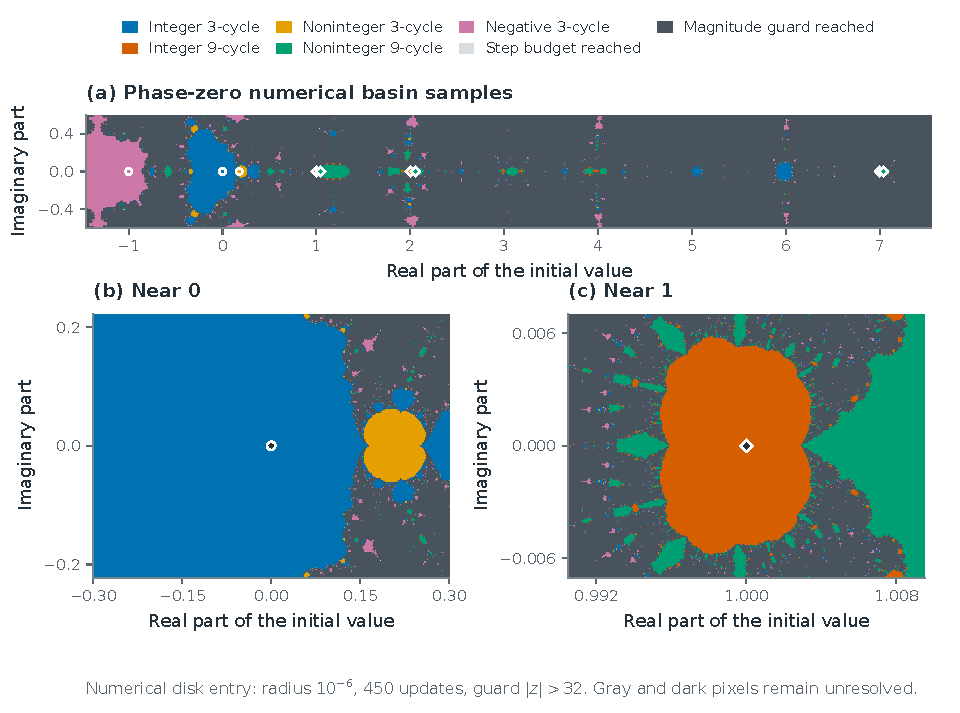
\includegraphics[width=.96\linewidth]{figures/complex_basins.pdf}
 \caption{Numerical basin views for the chosen cosine continuation
 at phase zero. The five target cycles have rigorous capture disks;
 the raster trajectories themselves are floating-point observations.
 Pixels reaching the magnitude guard or the iteration limit retain
 separate unresolved labels. Neither label proves divergence, and
 the five displayed attractors are not claimed exhaustive.}
 \label{fig:complex-basins}
\end{figure}

\FloatBarrier
\subsection{A real basin separator}

Put
$g(x)=R(x)-x$ for the return in \eqref{eq:complex-return}.

\begin{theorem}[Real separator]\label{thm:real-separator}
On $[0,9/50]$ the map $R$ is strictly increasing and has exactly
three fixed points: zero, a repeller
\[
 a\in(0.16503724,0.16503725),
\]
and an attractor
\[
 b\in(0.17752760,0.17752761).
\]
Every start in $[0,a)$ converges to zero under $R$, every start in
$(a,9/50]$ converges to $b$, and $a$ stays fixed. Moreover
$1.096<R'(a)<1.097$. The point $a$ lies on the boundary of both
corresponding open complex basins at phase zero.
\end{theorem}
\begin{proof}
The rational interval checker \path{certificates/geometry/separator.py}
covers the entire interval by closed subintervals and verifies
$R'>0$ on all of them. It verifies the following additional signs:
\begin{center}
\begin{tabular}{lll}\toprule
Interval&Strict sign&Number of certified subintervals\\\midrule
$[0,0.06]$&$g'<0$&6\\
$[0.06,0.15]$&$g<0$&5\\
$[0.15,0.17]$&$g'>0$&8\\
$[0.17,0.173]$&$g>0$&1\\
$[0.173,0.18]$&$g'<0$&4\\\bottomrule
\end{tabular}
\end{center}
At the two bracket endpoints for $a$, $g$ is respectively negative
and positive; at the two endpoints for $b$, it is respectively
positive and negative. Continuity and the strict monotonicity of
$g$ in those zones give exactly one zero in each bracket. Since
$g(0)=0$, the first two zones have no other zero. The remaining
strict signs exclude all other zeros in the interval. The derivative
enclosure on the first narrow bracket gives the repelling bound.
The second bracket is inside the independently certified capture
disk for the three-step noninteger orbit, identifying $b$ with that
orbit's phase-zero point.

The endpoint inequality $R(0.18)<0.18$ is checked directly, and
$R(0)=0$. Since $R$ is increasing, it preserves $[0,0.18]$ and an
iterate cannot cross a fixed point. For $0<x<a$, one has
$0<R(x)<x$; the decreasing orbit tends to a fixed point below $a$,
necessarily zero. For $a<x<b$, one has $x<R(x)<b$, so the orbit
increases to $b$. For $b<x\le0.18$, it decreases to $b$. Continuity
justifies the fixed-point property of each monotone limit.

The complex basins of zero and $b$ are open: each is a union of
preimages of an attracting neighborhood under continuous iterates
of $R$. Every complex neighborhood of $a$ contains real points
immediately to its left and right, belonging to these two different
basins. The repelling fixed point itself belongs to neither.
Consequently it is on both basin boundaries.
\end{proof}

The interval computation does not subtract two broad intervals to
estimate $g$ unnecessarily. On a box $[c-r,c+r]$ it encloses
$R'$ by the chain rule and uses
\[
 g([c-r,c+r])\subseteq g(c)+(R'([c-r,c+r])-1)[-r,r].
\]
For each physical step, the center value and derivative are bounded
by the same real Taylor method as above; the bound
$|C''|\le4+16(|c/2+1/4|+r/2)$ controls derivative variation on the
box. Every arithmetic interval is rounded outward to a rational
grid of denominator $10^{15}$. A failed strict comparison triggers
bisection, and an exhausted depth limit is an error. The saved leaf
intervals meet at their endpoints and cover each entire claimed
zone, so untested gaps cannot be hidden between sample points.

\begin{figure}[htbp]
 \centering
 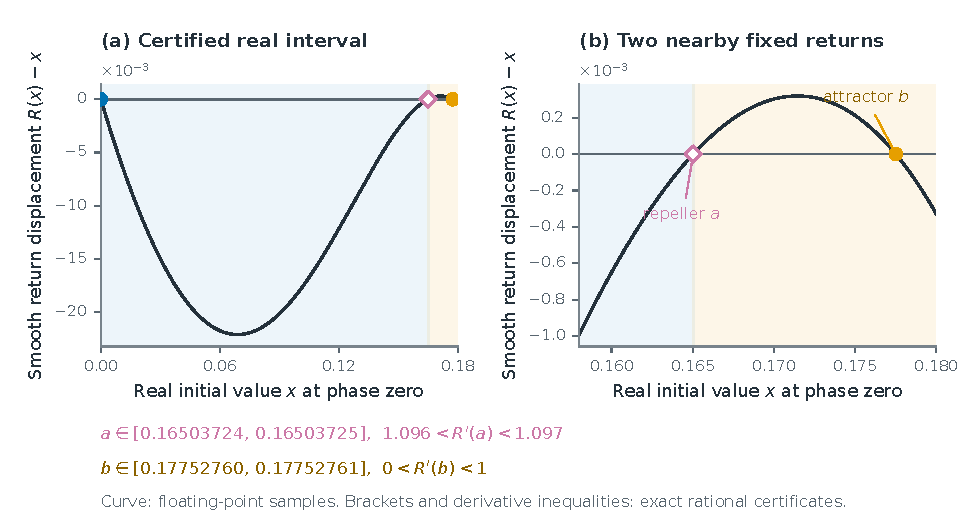
\includegraphics[width=.94\linewidth]{figures/real_separator.pdf}
 \caption{The phase-zero displacement $R(x)-x$ and the two nonzero
 root brackets. The curves are rendered numerically; the indicated
 signs, uniqueness of the three roots on $[0,0.18]$, and the basin
 partition are certified by the complete rational interval cover in
 Theorem~\ref{thm:real-separator}.}
 \label{fig:real-separator}
\end{figure}

\FloatBarrier
\subsection{The same complex point on three phase sheets}

Fix the complex starting point $w_*=71/100+\mathrm i/50$.

\begin{proposition}[Certified phase dependence]
\label{prop:complex-phase-dependence}
For the initial point $w_*$, launch phases zero and two converge
to the integer cycle $\Gamma_3$, whereas launch phase one converges
to $\Gamma_9$. The first entries into the radius-$10^{-6}$ disks
of the respective target cycles occur as follows:
\begin{center}
\begin{tabular}{rrrrl}\toprule
Launch phase&Updates&Arrival phase&Disk center&Destination\\\midrule
0&43&1&1&$\Gamma_3$\\
1&91&2&1&$\Gamma_9$\\
2&38&1&1&$\Gamma_3$\\\bottomrule
\end{tabular}
\end{center}
\end{proposition}
\begin{proof}
The checker \path{certificates/geometry/phase_trace.py} starts with
the radius-zero ball centered at the exact rational point $w_*$.
At every step it constructs a rational center $c_k$ and proves that
the true iterate lies in $|w-c_k|\le e_k$. Here is the error argument
that makes the finite calculation a certificate.

Reduce the real part of a center by its nearest integer and use
sine and cosine Taylor polynomials through degree 39 with rational
midpoint $\widehat\pi$. On the checked domain the reduced complex
argument has absolute value at most three. The tail is at most
$2\cdot3^{40}/40!$, by bounding successive exponential-series
terms geometrically. The uncertainty $\epsilon_\pi$ in $\pi$ adds
at most $8\epsilon_\pi$ to either trigonometric evaluation. The
constant eight follows from $|\operatorname{Im}w|<1/2$,
$\pi<4$, and the certified elementary bound $e^2<8$.
Write their combined bound as $\eta$.

The computed image polynomial is rounded to a rational center on a
$10^{-18}$ grid. Its rounding residual, together with
$|c_k/2+1/4|\eta$, bounds the error at the center. The analogous
derivative expression gives a rational upper bound $L_k$ on
$|C'(c_k)|$. Every enclosing disk satisfies
$|\operatorname{Im}w|<1/2$ and $|w|\le15$, on which
\eqref{eq:cosine-second} gives $|C''(w)|<2000$. Taylor's formula
along the segment inside the disk therefore permits the update
\begin{equation}\label{eq:complex-ball-error}
 e_{k+1}\ge \text{center residual}+L_ke_k+1000e_k^2.
\end{equation}
The checker rounds the right side upward to the $10^{-24}$ grid.
All remainder assumptions are verified again at every step; their
failure aborts the computation.

Let $r=10^{-6}$ and let $n$ range over the integer centers of the
target cycle on the current phase sheet. Before the claimed entry
time the checker verifies
$\min_n|c_k-n|^2>(r+e_k)^2$, excluding an earlier hit on those
disks. At the final time it verifies $e_k<r$ and
$\min_n|c_k-n|^2<(r-e_k)^2$, placing the entire error ball inside
a target disk. These are comparisons of rational numbers, without
square roots. The final errors are all less than $4\cdot10^{-18}$.
Proposition~\ref{prop:integer-capture-disks} then proves the
destinations in the table.
\end{proof}

All three terminal balls are near scalar height one. The first and
third are on phase one, where that integer belongs to $\Gamma_3$;
the second is on phase two, where it belongs to $\Gamma_9$.

\begin{figure}[htbp]
 \centering
 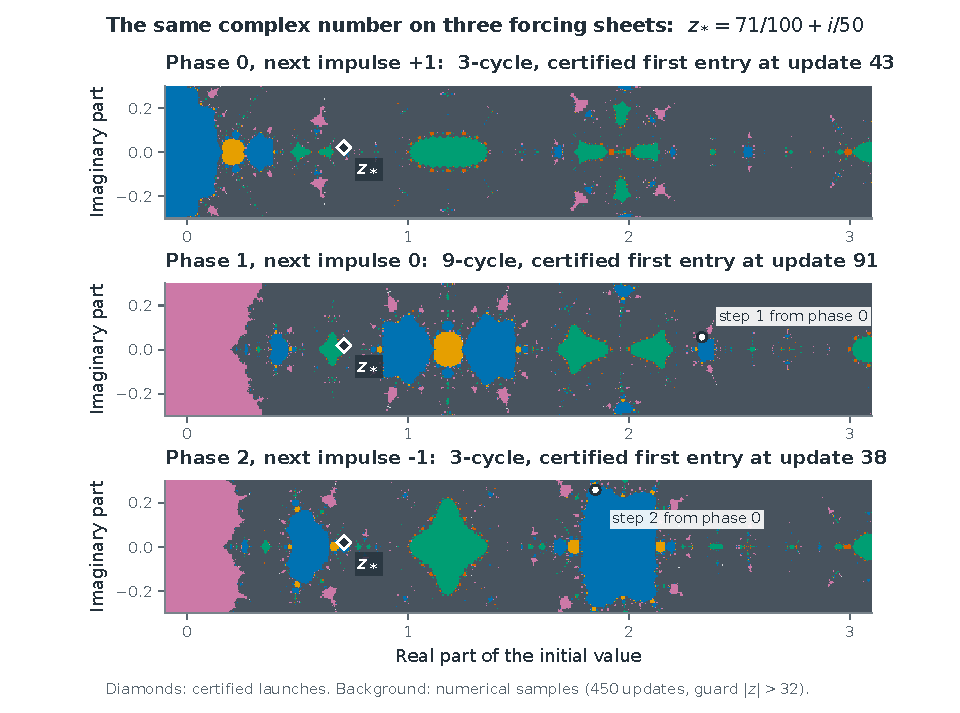
\includegraphics[width=.96\linewidth]{figures/phase_sheets.pdf}
 \caption{Three phase sheets of the same cosine continuation. Holding
 the complex coordinate fixed and changing sheets compares different
 launches; following a trajectory changes both its coordinate and its
 phase. The highlighted point $71/100+\mathrm i/50$ has the rigorously
 certified destinations and disk-entry times in
 Proposition~\ref{prop:complex-phase-dependence}. Background basin
 colors remain numerical samples.}
 \label{fig:phase-sheets}
\end{figure}

\subsection{Reproducing the geometry certificates}

Run
\begin{verbatim}
python3 -B certificates/geometry/verify.py
\end{verbatim}
with Python assertions enabled. The checker compares the eight integer
branches, three integer and two noninteger disk cycles, real interval
cover, and three complex-ball trajectories with
\path{certificates/geometry/certificate.json}. The figures sample a
finite grid. The total number of attractors remains open.

For the unforced cosine map, Lygeros and Rozier
\cite[Lemma~2.2]{lygeros-rozier-2014} provide a concrete link between
nearby real trajectories and integer orbits. With
$J_n^a=[n,n+a/(\pi^2n)]$, they prove
$C(J_n^a)\subseteq J_{T(n)}^a$ for all sufficiently large positive
integers $n$ when $27/8<a<6$, and for every positive $n$ when
$a=7/2$. A forced analogue would require intervals whose widths
depend on the phase. Translating the image by an impulse preserves
its width but changes the next center and denominator; those
inclusions and the small or zero centers would need new proofs.

\section{A fixed seven-step forcing}
\label{sec:seven-step}

Fix the impulse and height words
\[
 d=(0,0,1,-1,0,1,-1),\qquad
 h=(0,0,0,1,0,0,1),
\]
with $d_i=h_{i+1}-h_i$ and phase indices read modulo seven.
Write $F=F_d$ for the physical update in \eqref{eq:physical-forcing}, including at zero.
The safe domain

\[
 \mathcal D=\{(n,i):n\ge h_i\}
\]
contains every positive initial integer at every phase, together with
zero at the five phases where $h_i=0$.

By Proposition~\ref{prop:height-conjugacy}, $z=n+1-h_i$ evolves on
the positive integers under the repeated word $UUUTUUT$.

The phase-indexed physical values
\begin{equation}
 (c_0,c_1,c_2,c_3,c_4,c_5,c_6)=(0,0,0,1,1,2,2)
 \label{eq:seven-cycle}
\end{equation}
form a cycle: $T(c_i)+d_i=c_{i+1}$ at every phase.  In positive
coordinates its successive states are
\[
 (1,0),(1,1),(1,2),(1,3),(2,4),(3,5),(2,6).
\]
We say that a state is \emph{captured} if its forward orbit visits one
of the states $(c_i,i)$, and write $\operatorname{Cap}(n,i)$ for this
property.

\subsection{Section states and the exact open obligations}

Consider the section
\[
 \mathcal S=\{(z,i):z=3m,\ m\ge1,\ i\in\{3,5,6\}\}.
\]
For clarity, a pair $(m,i)$ in a section formula denotes the physical
state
\begin{equation}
 s(m,i)=(3m-1+h_i,i).
 \label{eq:seven-section-launch}
\end{equation}
Let $P$ denote the first \emph{strictly later} visit to $\mathcal S$.
A visit after a shrinking step counts.  Return existence will be proved
below, independently of capture.

The relevant natural-valued ranks are
\begin{align}
 V(m,3)&=V(m,5)=m,& V(m,6)&=2m,\\
 \rho(m,i)&=2V(m,i)+\mathbf1_{\{i=6\}}.
 \label{eq:seven-rho}
\end{align}
The same rank is used for all section phases simultaneously.

\begin{theorem}[Four-family conditional capture]
\label{thm:seven-four}
For the fixed forcing $d$, the following are equivalent.
\begin{enumerate}
\item Every positive physical integer, at every initial phase, is captured
by \eqref{eq:seven-cycle}.
\item Each of the following four statements holds:
\begin{align*}
 \mathrm{S00}:&\quad
 \operatorname{Cap}(s(4t+3,3))\quad &&\text{for every }t\ge0,\\
 \mathrm{S01}:&\quad
 \operatorname{Cap}(s(2t,5)) &&\text{for every }t\ge1,\\
 \mathrm{S02}:&\quad
 \operatorname{Cap}(s(32t+3,5)) &&\text{for every }t\ge0,\\
 \mathrm{S03}:&\quad
 \operatorname{Cap}(s(128t+115,5)) &&\text{for every }t\ge0.
\end{align*}
\end{enumerate}
In the second display, $\operatorname{Cap}(s(m,i))$ means capture of the
physical state defined in \eqref{eq:seven-section-launch}.  Equivalently,
every failure of capture would give a least-$\rho$ failure in this
four-family union.  None of the four universal hypotheses is discharged
by the theorem.
\end{theorem}

\subsection{Affine certificates on residue classes}

Every computational check in the reduction uses an input of the form
\[
 z=Aq+B,\qquad q\ge q_0,
\]
and propagates the two coefficients exactly.  When $A$ is even, every
input in this domain has the parity of $B$.  A physical shortcut step
therefore acts on the entire domain by
\[
 (a,b)\longmapsto
 \begin{cases}
 (a/2,b/2+d_i),&b\text{ even},\\
 (3a/2,(3b+1)/2+d_i),&b\text{ odd}.
 \end{cases}
\]
Here $(a,b)$ are physical-coordinate coefficients; the checker first
substitutes $n=z-1+h_i$ and converts back after each step.  At a candidate
section phase, the free coefficient remains divisible by three.  Hence
membership in the section is decided for the entire domain by the
constant coefficient modulo three.  Safety is checked at $q_0$ together
with positivity of the coefficient.

For the entrance calculation we use $A=384=3\cdot2^7$ and at most
seven updates.  For the short-return calculation from phase $i$ we use
$A=3\cdot2^{L_i}$ and at most $L_i$ updates.  The factor $2^{L_i}$
fixes every required parity; multiplying by an odd integer at a step
does not consume any additional powers of two.  The factor of three
fixes all section tests.  Each computation therefore covers the full ray.

An affine inequality on $q\ge q_0$ follows by checking that its slope
is nonnegative and its value at $q_0$ is nonnegative; strict inequalities
are treated with the corresponding integer minimum.  A negative slope
cannot be discarded by testing only small $q$.  The complete residue
partitions below use $0\le B<A$, with $q_0=1$ when the initial positive
coordinate would otherwise be zero.

\subsection{Every orbit reaches the section}

Start at phase zero, with $z=384q+r$, $0\le r<384$.  Propagate the
physical recurrence until a section hit or the end of one period.
Exactly 370 residue domains hit the section.  The fourteen remaining
domains have the following full-period returns; the output is $aq+b$.
All entries in this table have $q\ge0$.
\begin{center}
\begin{tabular}{rrr|rrr}
\hline
$r$&$a$&$b$&$r$&$a$&$b$\\ \hline
3&27&2&195&9&5\\
9&9&2&201&3&2\\
44&81&11&236&27&17\\
67&9&2&259&27&20\\
108&27&8&300&81&65\\
131&27&11&323&9&8\\
172&81&38&364&27&26\\ \hline
\end{tabular}
\end{center}
In each row $a<384$ and $1\le b<r$.  An avoiding period therefore
strictly lowers the positive integer $z$.  Indefinite avoidance would
produce an infinite strictly decreasing sequence of positive integers,
which is impossible.  An arbitrary initial phase can be aligned to zero
in at most six updates if no earlier section hit occurs.  This proves
entry from every state in $\mathcal D$.  Applying entry after one
further physical update proves that $P$ is total on $\mathcal S$.

The fourteen returns also satisfy the common envelope
\begin{equation}
 z_{\mathrm{next}}\le f(z):=\frac{27z+220}{128},
 \qquad f\left(\frac{220}{101}\right)=\frac{220}{101}.
 \label{eq:seven-avoid-envelope}
\end{equation}
This follows row by row by comparing coefficients and constants.
The 370 exiting domains satisfy
\begin{equation}
 w_j z_{\mathrm{exit}}\le\frac{27}{8}z,
 \qquad (w_3,w_5,w_6)=(1,1,2),
 \label{eq:seven-exit-envelope}
\end{equation}
where $j$ is the phase of the first section hit.  The factor at phase six is two.

\subsection{All sufficiently long returns strictly descend}

From a phase-five section launch, either the section is hit during
alignment or the phase-zero value is at most $(3z+5)/4$.  From phase
six, its phase-zero value is at most $(3z+1)/2$.  These two bounds use
respectively two and one updates and follow from the four and two
fixed-parity domains.

If there is then one complete avoiding period before the next section
hit, composing these bounds with \eqref{eq:seven-avoid-envelope} and
\eqref{eq:seven-exit-envelope} gives
\begin{align}
 w_jz_{\mathrm{exit}}
 &\le\frac{2187z+27405}{4096}<z
 &&\text{from phase five, if }z\ge15,\\
 w_jz_{\mathrm{exit}}
 &\le\frac{2187z+12609}{2048}<2z
 &&\text{from phase six, if }z\ge9.
 \label{eq:seven-long-bounds}
\end{align}
For example, the first strict inequality is equivalent to
$1909z>27405$ and holds already at $z=15$.  Its left-hand side
increases thereafter.  The second is equivalent to $1909z>12609$
and holds at $z=9$.

These estimates cover arbitrarily many avoiding periods.  Indeed,
the initial alignment upper bound is above $220/101$ at the stated
threshold.  Since $f$ is increasing and contracts towards that fixed
point, $f^k(B)\le f(B)$ for every $k\ge1$ and every such initial
bound $B$.  Applying the weighted exit estimate after the last avoiding
period therefore gives the same upper bound for every possible wait.

The last update of a phase-zero period ends at phase zero, which is
outside $\mathcal S$.  Consequently a return later than alignment
plus six updates entails a full avoiding period.  At phase three all
returns occur within three updates; the following complete table on
$m=8q+r$ verifies this directly:
\begin{center}
\begin{tabular}{rrrr}
\hline
$r$&output parameter&output phase&updates\\ \hline
0&$6q$&5&2\\
1&$6q+1$&5&2\\
2&$3q+1$&6&3\\
3&$18q+7$&5&2\\
4&$6q+3$&5&2\\
5&$6q+4$&5&2\\
6&$q+1$&6&3\\
7&$18q+16$&5&2\\ \hline
\end{tabular}
\end{center}
Here $q\ge1$ in the first row and $q\ge0$ in the others.
Thus every first return failing to strictly decrease $V$, apart from
the explicitly handled small inputs, occurs within the caps
\begin{equation}
 L_3=3,\qquad L_5=8,\qquad L_6=7.
 \label{eq:seven-caps}
\end{equation}
The small inputs outside the thresholds in \eqref{eq:seven-long-bounds}
have the exact returns
\begin{center}
\begin{tabular}{rrr}
\hline
launch $(m,i)$&return $(m',j)$&updates\\ \hline
$(1,5)$&$(1,5)$&7\\
$(2,5)$&$(3,6)$&1\\
$(3,5)$&$(9,3)$&5\\
$(4,5)$&$(6,6)$&1\\
$(1,6)$&$(1,3)$&4\\
$(2,6)$&$(1,3)$&11\\ \hline
\end{tabular}
\end{center}
The eleven-update return from $(2,6)$ lowers $V$ from $4$ to $1$.

\subsection{A complete direct first-return classification}

Use the residue partitions $m=2^{L_i}q+r$ at phases $i=3,5,6$.
There are $8+256+128=392$ infinite input domains.  The exact propagation
described above stops at the first later section visit.  Domains that
have not returned by their cap are covered by the long-return proof.
All other outputs are affine in $q$, so their rank differences can
be classified on the entire legal ray.

The six direct growing families are as follows.  Parameters are
nonnegative except for S01, where $t\ge1$.
\begin{center}
\begin{tabular}{llllr}
\hline
ID&launch $(m,i)$&return $(m',j)$&$V_{\rm out}-V_{\rm in}$&updates\\ \hline
S00&$(4t+3,3)$&$(9t+7,5)$&$5t+4$&2\\
S01&$(2t,5)$&$(3t,6)$&$4t$&1\\
S02&$(32t+3,5)$&$(81t+9,3)$&$49t+6$&5\\
S03&$(128t+115,5)$&$(243t+220,5)$&$115t+105$&7\\
S06&$(16t+7,6)$&$(81t+36,3)$&$49t+22$&4\\
S08&$(64t+15,6)$&$(243t+58,5)$&$115t+28$&6\\ \hline
\end{tabular}
\end{center}
These labels match the certificate files. The six families occupy
respectively $2,128,8,2,8,2$ of the fixed-modulus input domains.
Nine domains require the long-return argument.  On every other domain
the first return strictly lowers $V$, except possibly at the three
individual launches
\begin{equation}
 (m,i)=(1,3),(2,3),(1,5).
 \label{eq:seven-finite-base}
\end{equation}
For a domain containing one of these launches, every larger parameter
strictly descends.

The exact chains
\[
 (1,3)\xrightarrow{2}(1,5),\qquad
 (2,3)\xrightarrow{3}(1,6)\xrightarrow{4}(1,3)
               \xrightarrow{2}(1,5)
\]
settle \eqref{eq:seven-finite-base}; the arrows count literal updates.
The launch $(1,5)$ lies on the cycle \eqref{eq:seven-cycle} and
returns to itself after seven updates.

For an illustration of a whole growing-parameter case that the rank
already resolves, the first return
\[
 (64t+63,6)\longmapsto(81t+80,5),\qquad t\ge0,
\]
has an unweighted parameter increase but a strict $V$-decrease
$47t+46$, so this launch cannot minimize the rank of an uncaptured state.

\subsection{A merger closes the two phase-six induction cases}

Suppose $m=4q+3$ and set $x=3m=12q+9$, so $x\equiv1\pmod4$.
The positive-coordinate launch $(x,6)$ follows its prescribed two
steps as
\[
 (x,6)\longmapsto\left(\frac{3x+1}{2},0\right)
       \longmapsto\left(\frac{9x+3}{4},1\right).
\]
The alternative section launch $(2x,5)$ follows three prescribed
steps as
\[
 (2x,5)\longmapsto(3x,6)
       \longmapsto\left(\frac{9x+1}{2},0\right)
       \longmapsto\left(\frac{9x+3}{4},1\right).
\]
The indicated parities follow from $x\equiv1\pmod4$.  Both histories
are positive and meet at the same integer and the same phase.  In
physical coordinates this common state is $(27q+20,1)$.  Their future
orbits therefore agree, although their elapsed times differ.

The old ranks of the launches tie, but the refined rank has
\begin{equation}
 \rho(m,6)-\rho(2m,5)=(4m+1)-4m=1.
 \label{eq:seven-merger-gap}
\end{equation}
Both S06 and S08 satisfy $m\equiv3\pmod4$ throughout their domains.
Their alternate section parameters are respectively $32t+14$ and
$128t+30$, at phase five.  Their common positive-coordinate states
are respectively $(108t+48,1)$ and $(432t+102,1)$.

Every old strict $V$-decrease survives this refinement.  Indeed,
$V(a)-V(b)\ge1$ implies
\[
 \rho(a)-\rho(b)
 =2\bigl(V(a)-V(b)\bigr)+\mathbf1_{\{i_a=6\}}
                         -\mathbf1_{\{i_b=6\}}\ge1.
\]
This argument covers all long returns as well as the short affine
domains.  It does not cover equal-$V$ transitions automatically.  In
particular, the finite step $(2,3)\to(1,6)$ increases $\rho$ from
$4$ to $5$; it is valid because its explicit finite capture chain
has already been proved, not because it decreases the rank.

The table counts fixed-modulus domains after the merger. The column labelled ``finite'' counts
domains with a single exceptional base input; the rest of such a
domain strictly descends.
\begin{center}
\begin{tabular}{rrrrrrr}
\hline
phase&domains&forward&long&merger&residual&finite\\ \hline
3&8&4&0&0&2&2\\
5&256&113&4&0&138&1\\
6&128&113&5&10&0&0\\ \hline
\end{tabular}
\end{center}
Thus no least-$\rho$ failure can occur at phase six.  This does not
remove S01 automatically: its phase-six return has greater rank
than the original S01 launch.  Any composed rule must be compared
against the original rank.

\begin{proof}[Proof of Theorem~\ref{thm:seven-four}]
Every launch in the four hypotheses is a positive physical state,
so universal positive-seed capture implies the four hypotheses.
For the converse, assume them.  If any state in $\mathcal D$ failed
capture, section entry would provide a failed section state.  Choose
one of least natural-valued rank $\rho$.  It is not one of
\eqref{eq:seven-finite-base}, since those states are captured.
It is not in S00--S03 by hypothesis.  Every other section state
either has a strict rank-decreasing forward return, or belongs to
S06 or S08 and has a phase-correct merger with the smaller-ranked
alternative launch above.  In either case the smaller state has
the same failed future.  This contradicts minimality.  Hence every
state in $\mathcal D$, and in particular every positive physical
seed at every phase, is captured.
\end{proof}

For each remaining launch $a$, it suffices to show capture or exhibit a
section launch $b$ with $\rho(b)<\rho(a)$ and $F^u(a)=F^v(b)$ for
some $u,v\ge0$. Equality includes the phase. Shaw's impure integers
have a smaller positive predecessor under the unshortened odd update
$3n+1$ \cite[Definition~2.1 and Theorem~3.1]{shaw-2006}. Here the two
orbits may meet later, at different update counts, and $\rho$ compares
their initial states.

\subsection{Optimality of direct phase-affine ranks}

\begin{proposition}[Six direct growing domains are unavoidable]
\label{prop:seven-six-barrier}
There is an explicit set of eleven pairwise disjoint first-return
affine domains of $P$ such that, for every choice of positive real
weights $w_3,w_5,w_6$ and fixed real constants $c_3,c_5,c_6$, the
rank $R(m,i)=w_i m+c_i$ strictly increases on an infinite tail of at
least six of those domains.  For $V$, exactly the six S-domains in
this witness set grow; the complete classifier above has no other
growing tails.
\end{proposition}

\begin{proof}
In addition to the six S-domains already listed, the following five
domains are first returns.  All parameters are nonnegative except
for D35, where $t\ge1$.
\begin{center}
\begin{tabular}{lllr}
\hline
ID&launch $(m,i)$&return $(m',j)$&updates\\ \hline
D53&$(32t+31,5)$&$(27t+27,3)$&5\\
D35&$(4t+1,3)$&$(3t+1,5)$&2\\
D36&$(8t+2,3)$&$(3t+1,6)$&3\\
D65&$(8192t+6239,6)$&$(6561t+4999,5)$&13\\
D56&$(256t+147,5)$&$(81t+47,6)$&8\\ \hline
\end{tabular}
\end{center}
These eleven domains are pairwise disjoint: at a common phase their
residues disagree modulo the greatest common divisor of their input
moduli.  The bundled checker verifies their exact parities, safety,
endpoints, and absence of earlier section visits on every parameter.

For a branch $(Mt+r,i)\to(At+b,j)$ the leading coefficient of
$R_{\mathrm{out}}-R_{\mathrm{in}}$ is $w_jA-w_iM$.
If every coefficient on a directed phase cycle were nonpositive,
multiplying the inequalities would force the product of the
unweighted slopes $A/M$ to be at most one.  The following six
edge-disjoint cycles violate that bound:
\begin{center}
\begin{tabular}{lr}
\hline
cycle&product of slopes\\ \hline
S03&$243/128$\\
S00, D53&$243/128$\\
S02, D35&$243/128$\\
S06, D36&$243/128$\\
S01, D65&$19683/16384$\\
S08, D56&$19683/16384$\\ \hline
\end{tabular}
\end{center}
Every product exceeds one.  Hence each cycle contains a domain
with a strictly positive leading rank change.  The fixed offsets
cannot remove growth on its infinite tail.  Disjointness gives six
different input domains.  For $V$, the six S-domain leading changes
are positive and the five D-domain leading changes are negative.
The complete direct classification already excludes other growing
tails.
\end{proof}

The cycles constrain the rank weights. Their guards need not form
periodic trajectories. The count concerns the specified disjoint
domains on this section and leaves residue-dependent ranks, later
returns, and mergers available.

\begin{figure}[tbp]
\centering
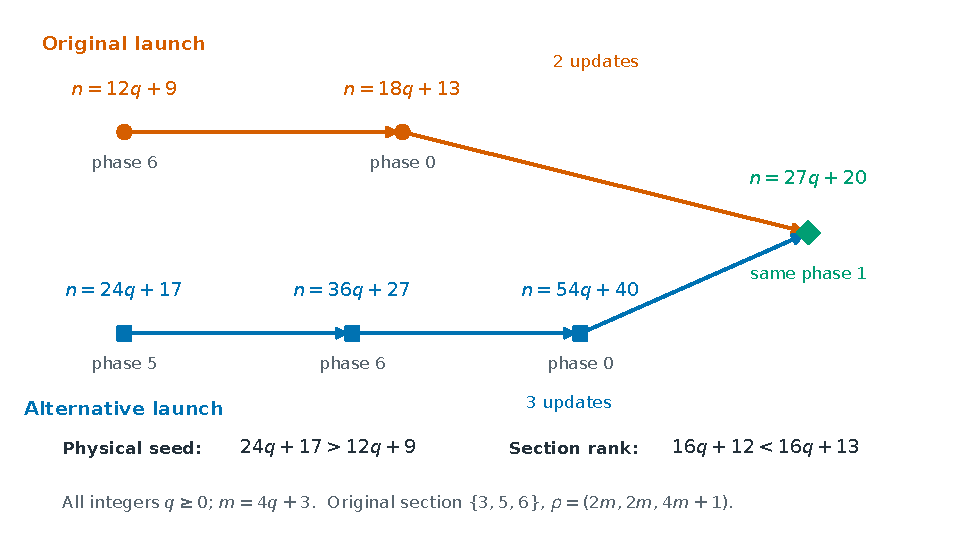
\includegraphics[width=0.93\linewidth]{figures/seven_step_merger.pdf}
\caption{The phase-correct merger used by the four-family reduction.
The two histories reach the same augmented state after different numbers
of updates. Their launch ranks differ by exactly one in $\rho$.
This figure concerns $\mathcal S$ and $\rho$; the alternative section
and rank in Section~\ref{sec:seven-three} are separate constructions.}
\label{fig:seven-merger}
\end{figure}

\paragraph{Reproduction.} Run
\begin{verbatim}
python3 certificates/seven_step/verify.py
python3 certificates/seven_step/test_mutations.py
\end{verbatim}
The first command reconstructs the physical certificates, compares
every field with the stored data, and checks an independent $T/U$
reconstruction on all fourteen phase--parity combinations. The second
tests rejection of defective and empty certificates. Both require
assertions enabled. The arbitrary-wait bound and least-rank induction
are written proofs.

\subsection{A second section with three residual families}
\label{sec:seven-three}

For the same forcing word and destination cycle take

\begin{equation}\label{eq:seven-new-section}
\begin{gathered}
 \mathcal S_* = \{(z,i):z=3m,\ m\ge1,\ i\in\{1,2,3,5\}\},
 \\
 W(m,i)=w_i m,\quad (w_1,w_2,w_3,w_5)=(4,7,4,5).
\end{gathered}
\end{equation}
The physical launch is still $s(m,i)=(3m-1+h_i,i)$, now with the
four indicated phases.  Write $P_*$ for the first strictly later visit
to $\mathcal S_*$.

\begin{theorem}[Three-family conditional capture]\label{thm:seven-three}
Every positive physical integer at every initial phase is captured by
\eqref{eq:seven-cycle} if and only if all three following statements hold:
\begin{align*}
 \mathrm{B1}:&\quad \operatorname{Cap}(s(2t,1)) &&(t\ge1),\\
 \mathrm{A3}:&\quad \operatorname{Cap}(s(4t+3,3)) &&(t\ge0),\\
 \mathrm{N03}:&\quad \operatorname{Cap}(s(8t+2,5)) &&(t\ge0).
\end{align*}
Every safe orbit enters $\mathcal S_*$ within eleven updates, and all
first returns from phases $1,2,3,5$ occur within $2,7,6,7$ updates,
respectively.  Outside the three families and five explicitly captured
states, $P_*$ strictly decreases the single natural-valued rank $W$.
The theorem does not prove any of the three universal capture hypotheses.
\end{theorem}

\paragraph{Uniform entry and bounded return.}
For entry, partition the phase-zero positive coordinate as
$z=1536q+r$, $0\le r<1536$, with $q\ge1$ for $r=0$ and $q\ge0$
otherwise.  The coefficient $1536=3\cdot2^9$ has more than enough
powers of two for five exact updates and retains a factor of three
throughout.  Consequently both parity and section membership are
constant on every propagated affine domain.  Independent physical
propagation gives the complete entry-time distribution
\[
 \begin{array}{c|rrrr}
 \text{first entry time}&1&2&3&5\\\hline
 \text{number of residue domains}&1024&384&64&64.
 \end{array}
\]
The counts sum to 1536.  Alignment from an arbitrary launch phase to
phase zero costs at most six updates, proving the stated bound of eleven.

For first returns, start with the entire domain $z=3m$ at each marked
phase.  Whenever the next parity is not fixed, split the free parameter
into its even and odd cases.  A growing branch $G$ and a shrinking branch
$S$ in the positive coordinate have the formulas
\[
 G_i(z)=\frac{3z+h_i}{2}\quad(z\equiv h_i\pmod2),\qquad
 S_i(z)=\frac{z+1-h_i}{2}\quad(z\not\equiv h_i\pmod2).
\]
These formulas describe branches of the prescribed $T/U$ schedule;
the branch is determined by the input parity. After $g$ growing updates,
the free coefficient is $3^{g+1}$: each parity split supplies the factor
of two consumed by that update. It is odd and divisible by three,
justifying the next split and the constant test for section membership.
Stop a domain at its
first later marked phase with $3\mid z$.  This procedure terminates
within the stated caps and produces the 43 domains in
Table~\ref{tab:seven-three-cylinders}.  At each source phase the
domains are pairwise disjoint and their dyadic widths sum to one.
Since all moduli are powers of two and bounded by the corresponding
$2^{L_i}$, this is an exhaustive finite partition of the positive
integers, not a density-only coverage claim.

As a separate reconstruction, partition $m$ modulo $2^{L_i}$ with
$(L_1,L_2,L_3,L_5)=(2,7,6,7)$, and propagate the original physical
recurrence, checking safety and the absence of an earlier section hit.
There are $4+128+64+128=324$ full-modulus input domains.  Each reproduces
the endpoint and time of its unique adaptive domain.  The two procedures
share the forcing and the section definition, but use different
coordinates and different partitions.

\begingroup
\small
\setlength{\tabcolsep}{7pt}
\begin{longtable}{rllllr}
\caption{The complete first-return partition for $\mathcal S_*$. All rows have
$t\ge0$, except $t\ge1$ when the displayed input is a multiple of $t$
with zero constant. The trace records every update, so its length is the
return time. The final column is $W_{\rm out}-W_{\rm in}$.}
\label{tab:seven-three-cylinders}\\
\toprule
$i$&input $m$&output $(m',j)$&trace&rank change&updates\\\midrule
\endfirsthead
\toprule
$i$&input $m$&output $(m',j)$&trace&rank change&updates\\\midrule
\endhead
\bottomrule
\endfoot
1&$2t$&$(3t,2)$&\texttt{G}&$13t$&1\\
1&$4t+1$&$(3t+1,3)$&\texttt{SG}&$-4t$&2\\
1&$4t+3$&$(t+1,3)$&\texttt{SS}&$-12t-8$&2\\
2&$2t$&$(3t,3)$&\texttt{G}&$-2t$&1\\
2&$8t+3$&$(9t+4,5)$&\texttt{SGG}&$-11t-1$&3\\
2&$8t+5$&$(3t+2,5)$&\texttt{SSG}&$-41t-25$&3\\
2&$8t+7$&$(3t+3,5)$&\texttt{SGS}&$-41t-34$&3\\
2&$64t+1$&$(9t+1,1)$&\texttt{SSSSGG}&$-412t-3$&6\\
2&$64t+17$&$(3t+1,1)$&\texttt{SSSSSG}&$-436t-115$&6\\
2&$64t+25$&$(9t+4,1)$&\texttt{SSSGGS}&$-412t-159$&6\\
2&$64t+33$&$(3t+2,1)$&\texttt{SSSSGS}&$-436t-223$&6\\
2&$64t+41$&$(9t+6,1)$&\texttt{SSSGSG}&$-412t-263$&6\\
2&$64t+49$&$(t+1,1)$&\texttt{SSSSSS}&$-444t-339$&6\\
2&$64t+57$&$(27t+25,1)$&\texttt{SSSGGG}&$-340t-299$&6\\
2&$128t+9$&$(9t+1,2)$&\texttt{SSSGSSG}&$-833t-56$&7\\
2&$128t+73$&$(3t+2,2)$&\texttt{SSSGSSS}&$-875t-497$&7\\
3&$4t$&$(3t,5)$&\texttt{SG}&$-t$&2\\
3&$4t+1$&$(3t+1,5)$&\texttt{GS}&$-t+1$&2\\
3&$4t+3$&$(9t+7,5)$&\texttt{GG}&$29t+23$&2\\
3&$32t+2$&$(9t+1,1)$&\texttt{SSGGS}&$-92t-4$&5\\
3&$32t+6$&$(3t+1,1)$&\texttt{SSSGS}&$-116t-20$&5\\
3&$32t+10$&$(9t+3,1)$&\texttt{SSGSG}&$-92t-28$&5\\
3&$32t+18$&$(27t+16,1)$&\texttt{SSGGG}&$-20t-8$&5\\
3&$32t+22$&$(9t+7,1)$&\texttt{SSSGG}&$-92t-60$&5\\
3&$32t+30$&$(3t+3,1)$&\texttt{SSSSG}&$-116t-108$&5\\
3&$64t+14$&$(3t+1,2)$&\texttt{SSSSSG}&$-235t-49$&6\\
3&$64t+26$&$(9t+4,2)$&\texttt{SSGSSG}&$-193t-76$&6\\
3&$64t+46$&$(t+1,2)$&\texttt{SSSSSS}&$-249t-177$&6\\
3&$64t+58$&$(3t+3,2)$&\texttt{SSGSSS}&$-235t-211$&6\\
5&$8t$&$(9t,1)$&\texttt{GSG}&$-4t$&3\\
5&$8t+2$&$(27t+7,1)$&\texttt{GGG}&$68t+18$&3\\
5&$8t+3$&$(9t+4,1)$&\texttt{SGG}&$-4t+1$&3\\
5&$8t+5$&$(3t+2,1)$&\texttt{SSG}&$-28t-17$&3\\
5&$8t+6$&$(9t+7,1)$&\texttt{GGS}&$-4t-2$&3\\
5&$8t+7$&$(3t+3,1)$&\texttt{SGS}&$-28t-23$&3\\
5&$16t+4$&$(3t+1,2)$&\texttt{GSSS}&$-59t-13$&4\\
5&$16t+9$&$(3t+2,2)$&\texttt{SSSG}&$-59t-31$&4\\
5&$16t+12$&$(9t+7,2)$&\texttt{GSSG}&$-17t-11$&4\\
5&$32t+17$&$(3t+2,3)$&\texttt{SSSSG}&$-148t-77$&5\\
5&$128t+1$&$(9t+1,5)$&\texttt{SSSSSGG}&$-595t$&7\\
5&$128t+33$&$(3t+1,5)$&\texttt{SSSSSSG}&$-625t-160$&7\\
5&$128t+65$&$(3t+2,5)$&\texttt{SSSSSGS}&$-625t-315$&7\\
5&$128t+97$&$(t+1,5)$&\texttt{SSSSSSS}&$-635t-480$&7\\
\end{longtable}
\endgroup


\paragraph{The finite exceptions and the induction.}
On a row $(Mt+r,i)\mapsto(At+b,j)$, the rank change is
\[
 W_{\rm out}-W_{\rm in}=(w_jA-w_iM)t+w_jb-w_ir.
\]
Exactly three rows have positive leading coefficient.  They are
\begin{center}
\begin{tabular}{llll}\toprule
Family&launch&first return&rank change\\\midrule
B1&$(2t,1)$&$(3t,2)$&$13t$\\
A3&$(4t+3,3)$&$(9t+7,5)$&$29t+23$\\
N03&$(8t+2,5)$&$(27t+7,1)$&$68t+18$\\\bottomrule
\end{tabular}
\end{center}
They grow on their whole legal domains.  Every other row has a negative
leading coefficient.  Solving its affine inequality on the entire legal
parameter ray leaves just
\[
 E=\{(1,1),(1,3),(1,5),(3,5),(5,3)\}
\]
as possible failures of strict descent.  Their capture times are
$4,2,0,14,16$ updates, respectively.  The first three have the physical
chains $(2,1)\to(1,2)\to(3,3)\to(4,4)\to(2,5)$ and its indicated
suffixes; $(2,5)$ is already on the destination cycle.  The longer two
chains, with phases advancing by one at each arrow, are
\begin{align*}
 (8,5):\quad&8,5,7,11,17,27,40,20,11,16,8,4,3,4,2,\\
 (15,3):\quad&15,22,11,18,8,4,2,2,0,0,1,1,2,1,3,4,2.
\end{align*}
Both end at phase five with physical value two.  The second chain
also illustrates why the convention at zero matters: it passes through
zero and continues, exactly as the forcing requires.

\begin{proof}[Proof of Theorem~\ref{thm:seven-three}]
The three families consist of positive physical states, so universal
capture implies their capture.  Conversely assume the three universal
statements.  If a safe orbit failed capture, uniform entry would give
a failed state in $\mathcal S_*$.  Choose such a state of least positive
integer rank $W$.  It is not in $E$, whose exact capture chains were
given above, and it is not in a residual family by hypothesis.
Its first return therefore strictly decreases $W$.  The return state
also fails capture, since its future is a suffix of the same orbit.
This contradicts minimality.  Every safe state is consequently captured.
\end{proof}

\paragraph{What changed relative to the four-family reduction.}
A3 is the old family S00.  At phase five, N03 is the subfamily
$m\equiv2\pmod8$ of the old even family S01.  The new section also
introduces B1 at phase one.  For the old S02 and S03 launches, it records
earlier endpoints
\[
 (32t+3,5)\xrightarrow{3}(36t+4,1),\qquad
 (128t+115,5)\xrightarrow{3}(144t+130,1).
\]
Their $W$-drops are $16t-1$ and $64t+55$.  The first is positive for
$t\ge1$; its remaining input $(3,5)$ belongs to $E$.  This explains
concretely how changing the section helps.  It does not prove capture
of those old families without the new hypotheses: a rank decrease
reduces an induction obligation but needs the common well-founded
argument to finish it.  Combining individual drops from $\rho$ and
$W$ without constructing one compatible order would not be valid.

\begin{proposition}[Three growing domains are optimal for this section]
\label{prop:seven-three-barrier}
Among positive phase-affine ranks
$R(m,i)=a_i m+b_i$ on $\mathcal S_*$, at least three of nine specified
disjoint first-return domains have a positive leading rank change.
The rank $W$ attains three growing domains in the complete 43-domain
partition.  The optimality assertion concerns this section and these
direct first-return comparisons.
\end{proposition}
\begin{proof}
Use the following three cycles of constraints, taking each labeled
edge from Table~\ref{tab:seven-three-cylinders}:
\[
 \begin{array}{c|c|c}
 \text{phase cycle}&\text{successive branch traces}&
       \text{product of slopes}\\\hline
 1\to2\to5\to1&G,\ SGG,\ GGS&243/128\\
 1\to3\to5\to1&SG,\ GS,\ GGG&243/128\\
 2\to3\to5\to2&G,\ GG,\ GSSG&243/128
 \end{array}
\]
Each edge is a different row of the disjoint partition.  If all three
leading rank changes in one cycle were nonpositive, multiplying
$a_jA\le a_iM$ around it would imply that the product of its slopes
$A/M$ is at most one.  Each displayed product is greater than one.
Thus each cycle contributes a different row with positive leading
coefficient; fixed offsets $b_i$ cannot cancel its growth for arbitrarily
large parameters.  The exact rank-change column proves attainment by
$W$.  These are cycles of inequalities on weights, not asserted
periodic trajectories satisfying every successive guard.
\end{proof}

\paragraph{Reproduction.}
\path{certificates/seven_step/three_family.py} regenerates
\path{three_family.json}, including the 43 affine rows, five finite
chains, independent physical reconstruction, entry times, and nine
obstruction witnesses. All 43 rows in \path{SevenRows.lean} agree with
the printed table after the parameter shift on zero-residue rows.

The Lean proof checks entry modulo 192 in at most six updates for
positive physical seeds at every phase. The eleven-update proof above
also covers safe zero states. Section~\ref{sec:formal-scope} gives the
formal three-family equivalence. The optimality proof above is written.


\section{A single remaining family and two approaches to its complement}
\label{sec:frontier-update}

Fix the seven-step word of Theorem~\ref{thm:seven-three}. In this section
$B(t)$ denotes the physical state $(6t-1,1)$, or equivalently the
normalized state $(6t,1)$, with $t\ge1$. Write $F$ for a physical
update. Heights at a meeting are compared at the same phase. The
two clocks that reach that phase may differ by a multiple of seven.
The \href{https://github.com/bruscaj/perturbed_collatz/tree/main/certificates/frontier}{public proof supplements}
give the full recurrence and interval arguments, exact certificates and
instructions for reproducing each computation.

\subsection{Entry and induction on the original B1 parameter}
\label{sec:b1-complement}

\begin{theorem}\label{thm:b1-complement}
Every safe phased state is captured by the distinguished cycle if and only
if $B(t)$ is captured for each positive $t$ outside the five guards below.
\end{theorem}

To see why a single family suffices, write the normalized height of an
arbitrary target as $27v+r$, $1\le r\le27$. For each phase and each $r$ the
entry certificate supplies $A,B>0$ and $k\le30$ such that the launch with
parameter $Av+B$ reaches that exact target after $k$ updates for every
$v\ge0$. The checker substitutes the affine ray into each signed update,
checking its parity, phase, safety and endpoint. These $7\cdot27$ identities
cover every positive normalized height. An ancestor can be larger than
its target. Its relevance is that once its trajectory enters the cycle,
the target on that trajectory also reaches the cycle. The Lean proof uses
a smaller table: first advance to phase one in at most six updates, then
use one of the 27 phase-one inverse rays to that aligned state.

Define $J(t)$ by the following disjunction. All variables in these
conditions are nonnegative integers. Put
\[
\begin{split}
 E={}&\{(1,1),(2,3),(4,1),(5,3),(6,1),(8,3),(9,1),(11,3),(12,1),(13,3)\},\\
 R={}&\{9,11,12,13,25,27,28,31,36,45,47,51,52,55,\\
     &\hspace{1em}61,66,69,71,82,83,85,99,104,107,108,120,123,127\}.
\end{split}
\]
\begin{enumerate}
\item $3\mid t$, $t=2^kq$, and $(k\bmod14,q\bmod4)\in E$.
\item $3\mid t$, $t=2^{14h+6}q$, and $59049^hq\equiv15\pmod{32}$.
\item $t=2^{24}v+1$.
\item $t\bmod128\in R$.
\item For some $h,r>0$ and $q\ge0$,
\[
 601t+151=128^h q,\qquad 729^h q=601(1+131072\,128^h r)+151.
\]
\end{enumerate}

\begin{proof}
Assume capture outside $J$. Induct strongly on $t$. The first two guards
give a merger with $B(t/3)$, using respectively $k+3$ and $14h+12$
ticks on both clocks. Exact divisibility is essential here. The third
gives capture at $t=1$ in 18 ticks and otherwise a merger with
$B(1179648v+1)$ at clocks 25 and 18. The fourth gives a direct seven-tick
return to a smaller positive parameter. The fifth gives a merger with
$B(1+131072\,9^h r)$ at clocks $14h+18$ and 18. The strict comparison
with the initial $t$ follows from the two counter equations and is proved
in the repayment arithmetic module. These are precisely the progress
lemmas used by \texttt{global\_capture\_iff\_final\_obligation} in the
frontier Lean project. Determinism transfers capture across each merger.
The ancestor cover now gives capture for the full safe domain.
Conversely, every B1 launch outside $J$ is a safe state.
\end{proof}

The entire ray $t=128v+19$ lies outside $J$. This gives a concrete test
of the theorem's remaining hypothesis. It is a statement about this
five-guard predicate. For example, $t=2^{28}v+19$ on that very ray has
a smaller partner under the two-clock rule below. The older three-family
result classifies minimum counterexamples using $W$. Its reductions may
change phase and use a different family as the smaller launch. Induction
on $t$ within B1 requires a positive smaller B1 parameter.

\subsection{A legal exit, repayment, and a partial selector}
\label{sec:legal-exits}

The 88-row cover uses five phases. Its rank, in phase order
$(1,2,3,5,6)$, is
\[ Q=(4m,8m,6m,6m,12m+3). \]
Its five growing labels are
N00, N01, N02, S00, and N03. Its stopping rule uses phases $1,2,5$ for
launches in those phases and the full five-phase set for the other
launches. The separate first-return calculation using all five marks
throughout has 32 rows. The physical checker replays both partitions.
The 43-row three-family classifier uses another section and the rank $W$.

As a concrete $W$ reduction in A3, take $t=16u+4$ and suppose
\[
 115u+36=2^{7h+5}q,\qquad 3^h q\equiv7\pmod 8 .
\]
The original section state $(4t+3,3)$ and the alternate $(3t+2,5)$
meet after $7h+14$ and $7h+12$ ticks. Their initial rank difference is
$4(4t+3)-5(3t+2)=t+2$. The proof factors the paired trajectories
through a component of seven modes with one positive affine counter.
The congruence selects its terminal merger. At $h=0$, $u=84$ gives a
meeting, while $u=20$ has the required valuation but misses the terminal
residue. A bound on time spent inside this component leaves reentry and
the other exits to be accounted for.

A different construction composes B1 returns. If a positive parameter
admits $k\ge1$ legal growing macros followed by $\lceil k/4\rceil$
legal contracting macros of the certified G/H pair, the resulting
parameter is positive and strictly smaller. Each macro spans seven
physical ticks. The theorem \texttt{certified\_ceil\_repayment} checks
the resulting clock, safety and comparison against the original rank.
The public selector combines a wider set of arithmetic rules and
returns a capture certificate, a smaller-parameter certificate, or an
unhandled outcome. A separate recurrent pair grammar permits arbitrarily
many successful packets with an outer decreasing parameter. Its renewal
calculation assigns density about $19.254724\%$ to successful neighbor
mergers on $t=128v+19$ within that grammar. This percentage describes
its acceptance language on that progression. Universal availability of
successful certificates remains open.

\subsection{Coalescence for almost every neighbor and its obstruction}
\label{sec:pair-coalescence}

Garner and Gao studied heights and consecutive starts for the ordinary
map \cite{garner-heights,gao-heights}. The paired-recurrence supplement
also credits Duran and Leen for ordinary-map synchronization work and
Lyapunov Weaver for the stopped-prefix argument adapted to phased B1.
For a fixed arithmetic progression of $t\ge2$, the set of $t$ for which
$B(t)$ and $B(t-1)$ meet at the same clock has relative natural density
one. The written argument tracks a pair at common phase as
$(x,3^e x+b)$, ordering the two slopes. Each next parity of the free
coordinate selects one of two dyadic subrays with equal conditional
weight. On the resulting countable chain of pair types, an offset estimate
and an excursion estimate for the exponent give almost-sure return to a
finite set. Each member has a finite merging word with positive
conditional probability. Repeated visits therefore yield absorption
with probability one. Finite successful words give entire integer rays.
Finite unions of these rays have their cylinder densities, which increase
arbitrarily close to one. The proof of the drift, finite-set hitting and
the passage to arithmetic progressions is supplied in the paired
recurrence supplement. The proof uses a distribution on rays, without a
randomness hypothesis about an individual orbit.

A separate equal-grow-count selector leaves $O(X^{29/30})$ possible
minimum representatives through $X$. This bound counts parameters for
which that selector fails to find a smaller partner by its specified
clock. Even within the known basin, infinitely many parameters have
no smaller equal-count, equal-clock partner at any clock. For a
captured parameter the excess-grow index
$I(t)=\lim_{m\to\infty}(g_{7m}(B(t))-2m)$ stabilizes because the cycle
has two growing steps per lap. Explicit embeddings send $I$ to
$I-12j$ for arbitrary $j\ge0$. Taking the least captured parameter in
each of these distinct classes gives the obstruction, since an
equal-count synchronous merger preserves $I$.

Allowing unequal clocks yields, for every $v\ge0$, the following two
identities. Endpoints below are in normalized coordinates $(z,p)$.
\[
\begin{array}{c|c|c|c}
t&\text{smaller }u&\text{clocks from }B(t),B(u)&\text{endpoint}\\\hline
2^{39}v+17&16\cdot3^{20}v+2&(39,4)&(564859072962v+21,5)\\
2^{28}v+19&204073344v+16&(28,7)&(2324522934v+183,1)
\end{array}
\]
Direct signed replay on each entire affine ray checks both clocks and
all intermediate parities. The search is exhaustive within its two clock
budgets and its requirement that the partner stride be at most the source
stride. These examples illustrate how a sparse set of unresolved
representatives can require a different proof for its individual members.

\subsection{Ancestors in intervals and the boundary of the basin}
\label{sec:inverse-intervals}

\begin{theorem}\label{thm:inverse-interval}
For each fixed $\delta>0$ there is an effective $M_\delta$ such that every
phased target of normalized height $z>0$ has an ancestor $B(t)$ with
$X<t<(1+\delta)X$ whenever $X\ge M_\delta z$.
\end{theorem}
\begin{proof}
Align the target to phase one by at most six inverse shrinking steps.
Writing $a=91/127$, a seven-shrink lap multiplies $z-a$ by 128. For
each residue modulo three an available one-grow inverse lap multiplies
$z-a$ by $L=128/3$ with additive error of absolute value below 30.
A 28-tick connector with three grows then reaches a B1 state. Its 81
ternary residue cases are checked as whole physical rays. With $C$
equal to the aligned positive height minus $a$ and $K=2^{27}/81$,
$j$ shrinking laps and $g$ one-grow laps give
\[
 t=K L^g(128^j C+e),\qquad |e|<1.
\]
Indeed the normalized lap error is at most $30/(L-1)=18/25$ and the
connector contributes at most $1/10$. As $\log_{128}3$ is irrational,
finitely many $3^{-g}$ modulo powers of 128 form a multiplicative
net of any fixed fineness. For $0<\delta\le1$, choose maximum successive
ratio at most $1+\delta/4$, then place the leading term between
$(1+\delta/4)X$ and $(1+\delta/4)^2X$. Since $C\ge36/127$, choosing
$X/z$ sufficiently large ensures $j\ge0$ and relative error below
$\delta/16$. The resulting parameter is strictly inside the required
interval. For larger widths use $\delta=1$. The interval supplement
gives the explicit threshold and the finite connector.
\end{proof}

\begin{corollary}\label{cor:cone}
Global capture is equivalent to the existence of a fixed $\delta>0$
and an unbounded sequence of intervals $[X,(1+\delta)X]$ on each of
which all B1 parameters have the same capture label.
\end{corollary}
\begin{proof}
Global capture makes every label one. Otherwise apply
Theorem~\ref{thm:inverse-interval} to a captured target and an uncaptured
target. Each sufficiently large interval of that width contains B1
ancestors of both. They inherit different labels from their targets.
\end{proof}

The interval construction can be combined with a positive inverse-tree
potential at exponent $17/20$. A prefix-free cut in the inverse tree of
a nonperiodic target gives disjoint branches. Applying the interval
constructor below each cut leaf gives at least
$c_\delta(X/z)^{17/20}$ distinct parameters for sufficiently large $X/z$.
For a periodic target, first pass to an off-cycle ancestor of bounded
height. This count requires the precision-14 potential inequalities;
the single-ancestor theorem and the corollary do not. Both labels
would inherit these abundance estimates if an exceptional basin exists.
Proving that the known label occurs throughout intervals of a fixed
relative width along an unbounded sequence remains an open problem.


\subsection{An alternative criterion at phase two}
\label{sec:affine-root}
Let $P(n)$ mean capture of normalized height $n>0$ at phase two. There is
a second conditional equivalence: global capture holds exactly when
$P(n)\Leftrightarrow P(27n-22)$ for every $n\ge1$. The right-hand
argument is larger even at $n=1$. Equality here concerns capture labels;
it permits distinct trajectories with the same final label.

Seven ticks take the phase-two pair $(128v+17,128v+19)$ to
$(27v+5,v+1)$ at phase two. Substituting $n=v+1$ identifies the assumed
label equality with the missing adjacent-odd link. Under this hypothesis
the odd-pair certificate connects whole congruence
classes of odd neighbors at phase two. Cutting the ordered odds at the
remaining edges produces an initial singleton and 33 periodic block
types. Split by parameter parity. Of the 66 types, 37 admit a direct
descent, 19 split into 2,432 affine rays in total, and ten use chains
of previously certified equalities. Each successful block comparison
ends below the original block minimum or at a checked finite base.
Induction gives capture on the odd blocks. The signed path identities
and the reduction of the remaining phased states are detailed in the
affine-root supplement. Conversely, global capture makes both labels
true for every $n$. The proof uses written induction and exact affine
checks. Establishing the displayed label equality for all $n$ remains
a distinct open problem.


\subsection{Which subsets and which phase comparisons suffice?}
\label{sec:phase-balance}

The ancestor theorem also admits a restriction on the launch parameter.
Let $S$ be a set of positive integers recognized by a finite automaton in
a fixed integer base, with positive upper natural density. Every target
has a B1 ancestor with parameter in $S$. The regular-domain supplement
constructs synchronized blocks and places them by inverse steering in
digit intervals where the automaton guarantees an accepting member.
As an explicit example, take $S$ to be the integers whose binary digit
sum is even. The arithmetic checker covers all 137,781 phase and residue
cases; one of the selected launches reaches the target in at most 30
updates. Consequently, proving capture on this one digit language would
suffice. Entry is certified; capture on the language remains open.

There is also a criterion that compares the same normalized height
across phases. Write $P_i(z)\in\{0,1\}$ for the actual capture
indicator of $(z,i)$. For each fixed pair $i\ne j$, global capture is
equivalent to $P_i(z)=P_j(z)$ at every positive height. Under the
assumed equality, a proof may substitute one of those labels for the
other. The phase-quotient supplement then uses transport of equal
labels and, where necessary, a complete dyadic partition, finite bases
and induction on height. A substitution in this argument is a logical
step; it adds no available update to the original fixed dynamics.

For $i<j$ set $e_{ij}(x)=P_i(x+1)-P_j(x+1)$, $x\ge0$. Exact affine
paths give identities of the form
\[
 e_{ij}(x)+\sum_{\ell}e_{ij}(a_\ell x+b_\ell)=0,
 \qquad a_\ell\ge2,\quad 0\le b_\ell<a_\ell.
\]
Each identity telescopes signed differences after the two ends of
each common affine ray are advanced through their forced updates.
The checker verifies all 21 pairs, using 294 edges. A nonzero
difference at $x\ge1$ therefore forces an opposite sign at some
strictly larger argument. All phases at $x=0$ are captured. Repeating
the argument shows that eventual absence of either sign for one full
phase pair would suffice for global capture. The argument does not
establish that either sign is scarce.

For a more restricted comparison, define
$A(t)=\mathbf{1}\{P_2(3t+3)>P_6(3t+3)\}$. If
$P_1(18v+2)\ne P_1(18v+3)$ then one of 35 affine arguments gives
a positive error of this restricted kind. The two directed paths have
14 and 21 edges. Both directions matter since either adjacent label can
be the positive one. For integer $X\ge1$ this gives
$N_J(X)\le35N_A(8192X)$, where $N_J(X)$ counts those disagreements
for $0\le v<X$ and $N_A(X)=\sum_{0\le t<X}A(t)$. This pointwise
transfer supplies a counting inequality even while both supports are
unknown.


The extra implication from $J$ to global capture needs its own evidence.
A 63-state ternary machine gives three checked transitions per state and
literal capture paths for all 63 base heights. The correction terms on
each transition are sums modulo two of adjacent errors $J$. If $A(t)=0$
for all $t\ge0$, the two directed paths above force $J(v)=0$ for every
$v\ge0$. All transition corrections then vanish. Induction on ternary
digits gives capture at phase two, and every other phase advances to
phase two in finitely many steps. Conversely, global capture makes
$A$ identically zero. This yields the restricted one-sided criterion
with its exact progression and sign; universal absence of that error
remains open.

\subsection{Classical coding and the precise forced model}
\label{sec:related-work}

The literature supplies several of the mechanisms used here. Write
$T(2k)=k$ and $T(2k+1)=3k+2$ for the shortcut map. Lagarias's
survey \cite{lagarias-1985} places parity coding, stopping times, inverse
trees, and generalized maps in their historical setting. For the ordinary
shortcut map, Terras \cite{terras-1976} proves the affine dependence of an
iterate on its initial value and the correspondence between finite parity
words and residue classes. Bernstein's explicit inverse coding
\cite{bernstein-1994} and the conjugacy developed by Bernstein and
Lagarias \cite{bernstein-lagarias-1996} describe the associated $2$-adic
dynamics. Proposition~\ref{prop:affine-parity} uses this classical
mechanism with a time-dependent intercept. Its contribution is the
explicit forced formula and its role in the subsequent certificates.

The companion generator in our height coordinate also has an exact
precedent. With $P(x)=x+1$, the map $U=PTP^{-1}$ is the map $E$ of
Monks et al.\ \cite[Section~3]{monks-et-al-2013}. Barina uses the same
translated map in an ordinary-trajectory batching algorithm
\cite[Section~3.1]{barina-2025}. The height proposition here establishes
which externally prescribed impulse words admit a binary height,
identifies their safe domain, and produces the resulting periodic
schedule of $T$ and $U$. The translated generator itself is inherited.

There are two distinct uses of periodicity in this subject. A map may
have coefficients periodic in the residue of its \emph{input}; our
impulses are periodic in \emph{time}, so the state includes the phase.
For a word of period $p$, a full return at a fixed phase is
residue-affine:
\[
 G(n)=\frac{3^{o_r}n+b_r}{2^p},\qquad n\equiv r\pmod{2^p}.
\]
This fits the independent-offset generalized class stated by Kionke
\cite[Section~1]{kionke-2017}. It should not automatically be identified
with every earlier definition of a generalized Syracuse map. In
particular, the original definition of Matthews and Watts
\cite[p.~167, equation~(1.3)]{matthews-watts-1984} uses a common system
of residue representatives, an additional restriction that need not
hold for a forced return. We use that source only for this checked
definition, rather than invoking a theorem from an uninspected portion
of its text.

The locally scaling shift theorem of Kingsbery et al.
\cite[Theorem~4.8 of the preprint]{kingsbery-et-al-2011} supplies a
further $2$-adic framework for these returns. Such coding concerns the
$2$-adic space, where a valid infinite itinerary need not represent a
positive integer. Akin's analysis of exceptional rational points
\cite{akin-2004} makes this distinction particularly relevant. Neither
a symbolic conjugacy nor the existence of every finite parity prefix
provides the real-size descent needed for integer capture.

\subsection{Stopping-time results and universal capture}
\label{sec:density-literature}

The natural-density first-descent theorem in Terras
\cite{terras-1976} and the logarithmic-density almost-bounded-orbit
theorem of Tao \cite[Theorem~1.3]{tao} have different conclusions from
capture of every seed. Tao allows any prescribed bound tending to
infinity and proves that the orbit minimum is below that bound outside
a set of logarithmic density zero. The possible exceptional set remains
material here: our conditional counting argument requires an upper
bound $o(X^\delta)$ for the exceptional set of the \emph{same forced
map}. Even a natural-density-one capture result would give only $o(X)$
exceptions, which does not supply that stronger comparison.

The intermediate thresholds also matter. Korec
\cite[Theorem~1]{korec-1994} obtains natural-density-one descent below
$n^c$ for each fixed $c>\log_4 3$. Inselmann's preprint
\cite[Corollary~1.4, arXiv v3]{inselmann-2024} gives, for every fixed
$\varepsilon>0$, the bound
$T^{\lfloor 2\log n/\log(4/3)\rfloor}(n)\leq n^\varepsilon$
on a set of natural density one. These ordinary-map statements distinguish
the size of the target, the density notion, and the iteration horizon.
Their transfer to our forced map would require an additional argument.
Shaik's recent preprint \cite[Theorem~1.1 and Section~8]{shaik-2026}
reports natural-density descent to a polylogarithmic target with an
arbitrary divergent multiplier, together with time and orbit-height
bounds. Its author reports a Lean proof of the main theorem and explicitly
distinguishes some registered corollary normalizations from the printed
ones. We have not independently rebuilt or axiom-audited that artifact;
these reported ordinary-map results are comparisons, not proof inputs.

For independent residue slopes, Venturini's published abstract
\cite{venturini-1997} states natural-density-one fixed-factor descent
in absolute value on each signed half-line, under positive coprime
branch numerators and geometric mean slope below one. Our period-$p$
return satisfies these stated algebraic conditions: the parity bijection
gives the slope product $(3/4)^{p2^{p-1}}<1$. The abstract allows a fixed
bounded alternative, which is absorbed by any fixed-factor bound for
sufficiently large inputs. The full proof was not recovered in this
review. This is a direct model comparison, but its conclusion supplies
neither capture nor descent below every prescribed divergent threshold.

Gon\c{c}alves, Greenfeld and Madrid
\cite[Definition~1.2 and Theorems~1.3 and~1.8 of arXiv v2]{goncalves-greenfeld-madrid-2025}
extend almost-bounded results to a
specified family of generalized Collatz maps. Their principal family
uses a fixed multiplier $q$ on the nonzero residue classes modulo a
fixed $p$, with positivity, integrality, coprimality, and the inequality
$q<p^{p/(p-1)}$; their natural-density power conclusion has additional
positive-offset hypotheses. Our full return generally has the different
multipliers $3^{o_r}$. Checking an average slope is therefore insufficient
to invoke their theorem. Applying it to this forced family would require
a proved reduction to their exact model.

Siegel and O'Dwyer's recent preprint
\cite[Theorem~5 and Definition~19, arXiv v1]{siegel-odwyer-2026}
reports an almost-boundedness theorem on number rings with varying
slopes. Its intended scalar conditions are compatible with our seven-step
return: $\rho_H=(3/4)^{448}$ and $127^2\rho_H<1$. This makes it a close
comparison, but we do not invoke its claimed theorem. The literal
global branch-integrality requirement in Definition~16 conflicts with
the coset-only condition in Definition~19, and the passage-probability
argument at the end of Section~7.2 requires further justification.
These are unresolved concerns about the inspected version, not a
counterexample to its intended conclusion. None of our capture
hypotheses is discharged by that preprint.

Kionke also states a one-dimensional eventual-periodicity conjecture for
coprime residue-affine maps whose product of absolute slope numerators
is smaller than the appropriate power of their denominator
\cite[Section~1]{kionke-2017}. That statement is a conjecture, not a
capture theorem available to close our residual families. It quantifies
over all signed integers. Even a future proof for every positive seed
of our fixed word would require a separate negative-domain analysis
before it could settle an instance in that form. The higher-dimensional
counterexamples in the same paper do not settle our one-dimensional
problem either.

\subsection{Inverse growth and arithmetic progressions}

Applegate and Lagarias \cite{applegate-lagarias-1995-i} develop finite
inverse-tree enumeration, including odd-step and congruence information,
as a way to obtain infinite lower counting bounds. Their second paper
\cite{applegate-lagarias-1995-ii} develops the difference-inequality
approach further. Krasikov and Lagarias
\cite[Theorems~2.2 and~6.1]{krasikov-lagarias} provide a soundness
framework and an ordinary-map lower exponent $0.84$ for positive targets
coprime to three. Our exponent between $0.535$ and $0.536$ concerns a
different, forced map and is not a numerical improvement to that result.
The model-specific work is the complete eligible branch census,
the forced affine offsets, distinctness across depths, the stopping
frontier, and the transfer to all safe targets and progressions.

The progression comparison is especially close. Monks
\cite{monks-2006} proves that every arithmetic progression is
sufficient for ordinary Collatz, in the sense of eventual merger with
an orbit from the progression. Monks et al.\ \cite{monks-et-al-2013}
develop admissible backtracing and stronger sufficiency statements.
These are direct antecedents of the affine residue steering used here.
Sufficiency does not assert that every forward orbit visits a given
progression. Their bounded odd-inverse count for targets coprime to
three also differs from the literal selector length needed here;
Section~\ref{sec:inverse} proves the size, multiplicity, and attachment
estimates required by our counting transfer.

A possible quantitative improvement is to retain more phase and residue
information in a system of forced inverse inequalities. The classical
inequality method suggests this experiment, but its soundness proof
would need the actual shifted arguments, eligibility guards, and
coverage of our return. Importing an ordinary-map recurrence or optimizing
unverified numerical weights would not establish a new exponent.

\subsection{Common control and synchronization}

Single-state steering, a common word for a finite ensemble, and periodic
capture from every phase are separate levels of control. Vasilyev's
recent preprint \cite[Section~4]{vasilyev-2026} studies the same available
upward and downward integer edges and gives closely related
single-state steering. A state-dependent choice of an edge does not
produce one temporal word that moves several states simultaneously.
We use a different notation for the translated companion $U$, so the
symbol $U$ in that preprint must not be identified with ours.

The pair-merging induction is classical in finite automata:
\v{C}ern\'y's criterion \cite[Theorem~2]{cerny-1964} reduces
synchronization to merging every pair. The arithmetic merger and
protected reference make that induction useful in our infinite state
space. The logarithmic dependence on the interval endpoint, with a word
chosen for that interval, and success of every cyclic rotation are
additional conclusions proved here, not consequences of the
finite-state criterion alone.

The probabilistic proof has the structure of drift and minorization
arguments used for geometric convergence \cite{rosenthal-1995}.
Shared random maps also occur in coupling from the past
\cite{propp-wilson-1996}, although our objective is word existence,
not exact sampling from a stationary distribution. Yano and Yasutomi
\cite{yano-yasutomi-2011} construct synchronizing random-map
realizations for finite ergodic chains. Here the maps and their common
coupling are prescribed, and the ensemble is not a finite reference
chain. We therefore prove the required ensemble estimates, reference
closure, and all-rotation union bound rather than infer them from
finite-chain mixing.

\subsection{Continuous geometry and inherited attraction}

The cosine continuation is Chamberland's function
\cite{chamberland-1996,chamberland-survey}; its interpolation is an
explicit modeling choice. Dumont and Reiter
\cite{dumont-reiter-2001,dumont-reiter-2003} already study real and
complex visualizations and alternative continuations. Agreement on
integer inputs leaves substantial freedom between them. In particular,
results about a chosen holomorphic extension, such as those of
Letherman, Schleicher and Wood \cite{letherman-schleicher-wood-1999},
cannot be transferred solely from their common integer values.

The general integer-cycle attraction proposition has a stronger prior
relationship than analogy. After the positive-height coordinate change,
the full-period return satisfies the hypotheses of Sindee, Sa
Ngiamsunthorn and Sriwongsa \cite[Theorem~3.3]{sindee-2024}.
Their extension and the positive-coordinate conjugate of our composed
cosine return have the same values and first derivatives at integers.
Section~\ref{sec:geometry} gives the
reduction and retains a direct multiplier proof. The general attraction
mechanism is therefore attributed as an application of existing work.
The particular trapping disks, noninteger cycles, real separator, and
phase-dependent complex trajectory still require the separate
certificates supplied here.

Lygeros and Rozier \cite{lygeros-rozier-2014} give shrinking real
intervals around integers for the unforced cosine map. A forced analogue
would be a useful next geometric theorem: specify interval widths at
each phase, prove inclusion under the actual translated update, and
handle the finitely many small centers. The original unforced
inequalities do not provide that inclusion after adding impulses.

\subsection{Finite certificates, termination, and formal proof}

The unresolved seven-step families can be viewed as a termination
problem on exact arithmetic domains. The size-change principle of
Lee, Jones and Ben-Amram \cite{lee-jones-benamram-2001}, and the
corrected development of monotonicity constraints by Ben-Amram
\cite[Section~3]{benamram-2010-monotonicity}, suggest finite graphs
whose edges certify comparisons of well-founded counters. To use this
method, each edge must hold on its entire guarded domain, every possible
execution must be covered, and the composed graph must force an infinite
descending thread along any putative infinite execution. Finding a
cycle in a residue graph, or checking only sampled parameters, does not
establish these conditions.

Transition invariants \cite{podelski-rybalchenko-2004} provide another
relevant design principle: a finite union of well-founded relations can
cover the transitive closure of the transition relation. Coverage of
execution segments is the substantive obligation. Path-complete graph
Lyapunov functions \cite{ahmadi-et-al-2014} similarly clarify why all
allowed products must be represented. Their matrix-system hypotheses
do not automatically cover guarded affine integer returns. An affine
lift must also account for offsets and the extra constant coordinate;
unconstrained matrix contraction is not supplied by a list of favorable
branch slopes.

Yolcu, Aaronson and Heule \cite[Section~3.2]{yolcu-aaronson-heule-2023}
give a mixed-base string-rewriting encoding whose termination is
equivalent to ordinary Collatz. Their negative results concern specified
classes of interpretations, not all termination methods. A forced
encoding would need its own phase representation, forward and backward
simulation, and proof that administrative rewriting cannot continue
forever without physical progress. Carelli's connection between
one-variable linear-constraint loops and weak generalized Collatz
reachability \cite{carelli-2026} is also conditional on an explicit
conjecture and an exact model. It is not an automatic decision procedure
for our guarded, multi-branch return.

Nashida's recent companion preprints
\cite{nashida-2026,nashida-2026-part-ii} address staged valuation
certificates and limitations of finite abstractions and matrix
interpretations. Their revision-r3 repositories report Lean coverage
of certificate soundness and five examples in Part~I, and seven
residue-avoidance weakenings in Part~II. The general dichotomy,
nonexistence results, matrix barriers, and maximality are outside the
reported formalization. We inspected those scope statements without
independently rebuilding or axiom-auditing the artifacts. A use for our
forced system would need its own faithful encoding and certificate
verification; the reported barriers concern their specified methods.

For certificate formalization, Gonthier's computational-reflection
architecture \cite{gonthier-2005} illustrates the essential separation:
prove a checker's semantic correctness, then use its accepted finite
data to obtain the mathematical statement. Solovyev and Hales
\cite{solovyev-hales-2013} provide an analytic example using Taylor
interval certificates. Our next Lean milestones are the corresponding
coverage and soundness theorems, not merely imports of recorded maxima
or successful external runs. The Lean infrastructure and its axiom and
validation guidance \cite{demoura-ullrich-2021,lean-axioms-424,
lean-validating-proofs} help describe that trust boundary; the exact
coverage of this repository is listed in Section~\ref{sec:formal-scope}.

Finally, the residue-affine literature gives useful limits on overly
simple descriptions. Kohl proves wildness of iterates for surjective
noninjective residue-class-wise affine maps \cite{kohl-2007}, and a
separate obstruction for a restricted class of monotonizing conjugacies
\cite{kohl-2008-conjugates}. These statements do not rule out
variable-time returns, relational mergers, residue-dependent ranks, or
finite certificates of entry. They support specifying the exact scope
of an obstruction before using it to discard a proof strategy.

\subsection{Contribution and review boundaries}
\label{sec:literature-boundaries}

The release combines a model-specific admissibility classification,
exact support bounds, an all-phase synchronization theorem, forced
inverse growth and progression transfer, explicit geometric
certificates, and conditional seven-step reductions. Their classical
coding, control, counting, interpolation, and verification ingredients
are attributed above and beside their uses. No general novelty claim
is made for those ingredients or for the inherited integer-attraction
principle. Priority for the precise forced statements remains a separate
review question.

The bibliography is selective, rather than a claim to enumerate every
Collatz paper. The accompanying staging audit accounts for all 88 entries
in the pre-existing source register, records additional sources, and
distinguishes inspected primary text from metadata or abstract-only
checks. In particular, the Matthews--Watts comparison above uses the
recovered definition; the Letherman--Schleicher--Wood comparison uses
the publisher abstract and the explicit distinction in Dumont--Reiter;
the Lee--Jones--Ben-Amram and Podelski--Rybalchenko references supply
historical and methodological context whose exact formal use would
require further source review. Full-text gaps and version discrepancies
remain visible in that audit. None is silently treated as a theorem
that closes the remaining capture hypotheses.

\section{Formal coverage, open obligations, and ordinary Collatz}
\label{sec:formal-scope}

\subsection{What has actually been formalized}

The release contains three independent projects for the Lean~4 theorem
prover \cite{demoura-ullrich-2021}. It preserves the twelve
mathematical source modules of the initial research snapshot and incorporates
six additional signed-model modules from the subsequently merged audit. A
separate release bridge states the positive-seed capture result as an
if-and-only-if theorem. Thus there are nineteen mathematical modules:
eighteen source-preserved modules and one explicitly identified release
bridge. The original sources are unchanged. The source pins, byte comparisons,
and packaging transformations are recorded outside the minimal export;
\path{lean/README.md} explains the public layout.

The inverse project now includes the general signed physical model,
admissibility, height coordinates, cycle gain, and the three-family reduction,
in addition to its original three-step inverse results. It uses Lean 4.24.0,
as does the sprint project. The perturbed project uses Lean 4.19.0. None
requires mathlib. A clean verification builds each project in a new temporary
directory, checks the exact toolchain version, treats audit warnings as errors,
and compares the regenerated theorem inventory with the committed one.

\begin{center}\small
\begin{tabular}{lrrrr}\toprule
Project&Mathematical modules&Public&Private&Audited constants\\\midrule
\texttt{inverse}&11&110&37&556\\
\texttt{perturbed}&6&86&43&401\\
\texttt{sprint}&2&5&0&33\\\midrule
Total&19&201&80&990\\\bottomrule
\end{tabular}
\end{center}
The public and private columns count named source theorem declarations.
The last column also includes elaborator-generated theorem constants.
Two hundred public declarations come from preserved research sources; the
release bridge adds one. These counts are not independent-result counts
or percentages of the manuscript completed. The separate
\path{SevenAdversarial.lean} fixture checks twenty-one malformed-row or
scope examples and is not counted as a mathematical module.

The inventory in \path{lean/inventory.json} stores exact elaborated theorem
types, source locations, and transitive axiom dependencies. Across all 990
audited constants, the dependencies are drawn only from
\texttt{propext}, \texttt{Quot.sound}, and \texttt{Classical.choice}; no
\texttt{sorryAx} or custom axiom occurs. The complete audit includes unused
private and generated theorem helpers. An external independent Lean kernel
checker has not been run. The compile-and-audit result does not certify
unconnected Python, C++, plotting code, or the entire written manuscript.

The permitted axioms and transitive dependency inspection are documented
in the versioned Lean reference \cite[Sections~8.4--8.5]{lean-axioms-424}.
Axiom inspection does not decide whether the elaborated definitions and
theorem statement express the intended mathematics. The official
proof-validation guide treats that as a separate obligation and
distinguishes dependency auditing from proof replay and independent
kernel checking \cite{lean-validating-proofs}. The model comparisons
below address the statement-matching obligation; no additional checker
run is claimed here.

\paragraph{Directly matching results.}
The conservative cyclic-alternation assertion is proved in
\path{Collatz.Physical.conservative_admissible_iff_alternating}.
For arbitrary signed forcing, \texttt{admissible\_iff\_floor} gives the
binary-floor formulation of admissibility; the particular separated-negative-
impulse formulation in Theorem~\ref{thm:admissibility} is still presented
with its written proof. The source also proves binary-height existence
and uniqueness, the exact safe domain under the nonzero-word hypothesis,
physical/positive-coordinate conjugacy, its orbit and cycle consequences,
and admissibility under phase rotation. The primitive-period comparisons
in the manuscript are not separately formalized.

The all-depth inverse-lap and binary-zoom identities have direct Lean
support. So does the arithmetic return inequality $3^o<2^L$ used in
Proposition~\ref{prop:integer-cycle-attraction}. The latter theorem is
about integer arithmetic and safe returns; complex differentiation and
local analytic attraction are further written arguments.

The main new formal conclusion is
\path{Collatz.ReleaseBridge.global_capture_iff_three}:
universal capture of positive physical integers at all phases is
\emph{equivalent} to capture of the three complete B1, A3, N03 families.
It uses the committed signed theorem
\path{Collatz.SevenStep.global_capture_of_three} for the substantive
implication and proves the converse from positivity of the family launches.
The order of coordinates in Lean is phase then integer. Its physical word,
continued-zero convention, target cycle, and family parameter domains match
Section~\ref{sec:seven-three}. All 43 source Lean rows were independently
compared with the printed and Python rows, including the parameter shift
needed on zero-residue classes. The formal entry result is at most six
updates for positive seeds; the separate eleven-update safe-domain bound
and the scoped rank-optimality argument retain their stated evidence.

The family assumptions are explicit hypotheses, not trusted axioms. A
checked implication does not make those hypotheses true. The formal
statement therefore remains conditional on the same open mathematics as
the written theorem, while checking that particular implication in the signed physical model.

\paragraph{Related models still require care.}
The older perturbed project contains useful constituent lemmas with
different conventions. In particular, \texttt{PerturbedCollatz.step}
makes zero absorbing, and its orbit-lift theorem requires positivity
along the original prefix. Its period-seven example uses
$(-1,0,0,1,0,0,0)$, not the word in Section~\ref{sec:seven-step}.
Its escaping-basin theorem assumes an escaping target instead of
constructing one. The older progression-steering result uses a modulus
$n+1$ coprime to six and also requires $3^n\mid z-c$. It is not the
arbitrary-target all-progression theorem in this manuscript.

The sprint project supplies root inverse-height and packet identities;
those auxiliary declarations do not prove the residual-family hypotheses.
Likewise, the new signed parity-lift theorem supplies a positive odd affine
multiplier, but does not by itself formalize the entire parity-word/residue
bijection or identify it as $3$ raised to the number of odd inputs. Read the exact types before
transferring any statement. The claim-to-evidence map distinguishes a full
matching conclusion from a supporting identity and a related model.

\subsection{What remains to formalize and what requires new mathematics}

The signed model and the conditional three-family conclusion are now
available as formal foundations for further work. A next extension can
reuse them rather than introducing another convention for zero, phase,
or physical height. The remaining tasks have distinct sizes and proof
requirements.

For inverse growth, formalize the complete 24-step branch minima and
eligibility inequalities, then prove cross-depth noncollision, the
weighted stopping-frontier bound, and the finite selector's size and
multiplicity estimates. Correct arithmetic on a finite list does not
supply the list's exhaustive coverage or those universal counting
arguments automatically.

For the support bounds, a formal certificate interface must justify the
arbitrary-gap reduction, the complete signed tail closure, the finite
core/complement split, and every upper-bound enumeration. Replaying an
attaining witness or importing a recorded maximum is insufficient. The
current independent C++/Python replays remain computational evidence
outside Lean. For synchronization, the unfinished formal work includes
the protected drift, exponential tail, closed-reference conditioning,
union bound over all rotations, and primitive-period argument.

The continuous geometry would require real and complex analysis plus a
sound rational interval and disk interpreter. The proof obligations are
Taylor remainder bounds, outward rounding, complete interval coverage,
contraction, and the relation between disk capture and basin membership.
The numerical figure generator supplies none of these proof obligations.
Solovyev and Hales \cite[Sections~2--3]{solovyev-hales-2013} give a
relevant precedent: an external search produces Taylor/interval
certificates, which theorem-producing procedures then verify in
HOL~Light. For this release, a Lean interpreter would have to prove
the meaning and soundness of the actual rational certificate records.
The existing Python checker does not supply that formal interpreter.
The four-family theorem also remains a separate formalization task: its
control of returns beyond the short verification caps and its phase-correct
alternative-launch mergers are not formalized by the separate three-family
proof.

\begin{center}\small
\begin{tabular}{p{.25\textwidth}p{.33\textwidth}p{.31\textwidth}}\toprule
Target&Current evidence&Remaining obligation\\\midrule
Three-family global equivalence&Signed Lean proof and release iff bridge;
independent affine reconstruction&Prove the three whole-family capture
hypotheses to obtain unconditional capture\\[4pt]
Full foundation statements&Conservative classification, height/safety,
conjugacy and arithmetic cycle gain in Lean&Exact general separation
formulation, full parity-cylinder bijection, primitive-period statements\\[4pt]
Inverse growth in every progression&Written proof and exhaustive 24-step
certificate&Formal coverage, noncollision, weighted counting,
finite selectors and multiplicity\\[4pt]
Support bounds and synchronization&Complete written arguments and exact
support censuses&Formal upper-bound reduction/enumeration and the
probabilistic all-phase proof\\[4pt]
Continuous geometry&Rational disks, interval leaves and trace balls;
written analytic proofs&Sound analytic interval/disk interpreter and
formal contraction/basin arguments\\\bottomrule
\end{tabular}
\end{center}

Each milestone should end with a theorem whose complete type is compared
with the manuscript. Closing a formalization gap proves that a stated
argument has been checked by Lean. Closing B1, A3, and N03 requires new
mathematics about all parameters in those families; additional build logs
or declaration counts cannot perform that step.

\subsection{What would be needed for ordinary Collatz}

Let $T$ be the unforced shortcut map on positive integers. Its conjecture
asserts that every such orbit reaches 1. The results here concern either
a designed forcing or one of two particular fixed forced maps. The
coordinate change of Section~\ref{sec:foundations} gives a periodic
schedule of $T$ and $U$; it does not remove that schedule to give ordinary
$T$ iterations. No reduction from unforced capture to either set of
seven-step obligations has been established in this manuscript.

For example, a future transfer argument could specify an encoding $E$
of every positive unforced seed, prove a simulation relation between
unforced iterates and returns of a forced map, and show that forced
capture of every encoded state implies unforced capture. Such an argument
must prove the clock correspondence, guard coverage, safe domain,
existence of all required returns, and transfer of the terminal cycle.
Another possible route would prove a sufficiently strong exceptional-set
upper bound for exactly the forced map of Corollary~\ref{cor:exceptional-set},
then separately establish a sound transfer to the ordinary map. Neither
route is supplied by empirical similarity, inverse-basin abundance,
or a finite family of successful starting values.

The logarithmic-density result of Tao \cite{tao} is an example of a
powerful ordinary-Collatz theorem whose conclusion still differs from
universal capture: almost all orbits, in logarithmic density, attain a
bound given by any function tending to infinity. That statement is not
the exceptional-set power bound required here, and it concerns another
map. The distinction between an almost-everywhere conclusion and an
all-seeds conclusion remains substantive.

The three residual families in Theorem~\ref{thm:seven-three}, or
alternatively the four in Theorem~\ref{thm:seven-four}, are explicit
next targets within this research program. Progress would consist of an
exhaustive compatible reduction of one complete set of families, a
different complete invariant, or a
proof of their capture. Additional reductions on proper subprogressions
can be useful, but leave infinite complements unless an explicit coverage
argument closes them. The current work supplies several independently
checkable results and a concrete conditional reduction; it does not
establish the classical conjecture or claim to solve another named open
conjecture without a separate implication and literature check.


% Bibliographic metadata and access limits are recorded in the staging literature audit.
\begin{thebibliography}{99}
\addcontentsline{toc}{section}{References}
\setlength{\itemsep}{1.5pt plus .5pt minus .5pt}
\bibitem{lagarias-1985}
Jeffrey C. Lagarias,
\emph{The $3x+1$ problem and its generalizations},
The American Mathematical Monthly 92(1), 3--23 (1985).
\url{https://doi.org/10.2307/2322189}.

\bibitem{terras-1976}
Riho Terras,
\emph{A stopping time problem on the positive integers},
Acta Arithmetica 30(3), 241--252 (1976).
\url{https://doi.org/10.4064/aa-30-3-241-252}.

\bibitem{bernstein-1994}
Daniel J. Bernstein,
\emph{A non-iterative 2-adic statement of the $3N+1$ conjecture},
Proceedings of the American Mathematical Society 121(2), 405--408 (1994).
\url{https://doi.org/10.1090/S0002-9939-1994-1186982-9}.

\bibitem{bernstein-lagarias-1996}
Daniel J. Bernstein and Jeffrey C. Lagarias,
\emph{The $3x+1$ conjugacy map},
Canadian Journal of Mathematics 48(6), 1154--1169 (1996).
\url{https://doi.org/10.4153/CJM-1996-060-x}.

\bibitem{monks-et-al-2013}
Keenan Monks, Kenneth G. Monks, Kenneth M. Monks, and Maria Monks,
\emph{Strongly sufficient sets and the distribution of arithmetic sequences in the $3x+1$ graph},
Discrete Mathematics 313(4), 468--489 (2013). Checked text: arXiv:1204.3904v2.
\url{https://doi.org/10.1016/j.disc.2012.11.019}.

\bibitem{barina-2025}
David Barina,
\emph{Improved verification limit for the convergence of the Collatz conjecture},
The Journal of Supercomputing 81, article 810 (2025).
\url{https://doi.org/10.1007/s11227-025-07337-0}.

\bibitem{kionke-2017}
Steffen Kionke,
\emph{A geometric approach to divergent points of higher dimensional Collatz mappings},
Monatshefte f\"{u}r Mathematik 182, 851--863 (2017).
\url{https://doi.org/10.1007/s00605-016-0947-4}.

\bibitem{matthews-watts-1984}
K. R. Matthews and A. M. Watts,
\emph{A generalization of Hasse's generalization of the Syracuse algorithm},
Acta Arithmetica 43(2),167--175 (1984).
\url{https://doi.org/10.4064/aa-43-2-167-175}.

\bibitem{kingsbery-et-al-2011}
James Kingsbery, Alex Levin, Anatoly Preygel, and Cesar E. Silva,
\emph{Dynamics of the p-adic shift and applications},
Discrete and Continuous Dynamical Systems 30(1), 209--218 (2011). Theorem numbering follows arXiv:0903.4226.
\url{https://doi.org/10.3934/dcds.2011.30.209}.

\bibitem{akin-2004}
Ethan Akin,
\emph{Why Is the $3X+1$ Problem Hard?},
Chapel Hill Ergodic Theory Workshops, Contemporary Mathematics 356, 1--20 (2004).
\url{https://math.sci.ccny.cuny.edu/document/Akin2004_WhyThreeXisHard.pdf}.

\bibitem{tao}
Terence Tao,
\emph{Almost all orbits of the Collatz map attain almost bounded values},
Forum of Mathematics, Pi 10, e12, 1--56 (2022).
\url{https://doi.org/10.1017/fmp.2022.8}.

\bibitem{korec-1994}
Ivan Korec,
\emph{A density estimate for the $3x+1$ problem},
Mathematica Slovaca 44(1), 85--89 (1994).
\url{https://dml.cz/dmlcz/133225}.

\bibitem{inselmann-2024}
Manuel Inselmann,
\emph{An Approximation of the Collatz Map and a Lower Bound for its Average Total Stopping Time},
Preprint, arXiv:2402.03276v3 (2024).
\url{https://arxiv.org/abs/2402.03276v3}.

\bibitem{shaik-2026}
Idris Ali Shaik,
\emph{Polylogarithmic Descent for Almost All Collatz Orbits in Natural Density},
Preprint, version 4.0.2 (4 October 2026).
\url{https://doi.org/10.5281/zenodo.23132901}.

\bibitem{venturini-1997}
G. Venturini,
\emph{On a Generalization of the $3x+1$ Problem},
Advances in Applied Mathematics 19(3), 295--305 (1997).
Publisher abstract and metadata inspected.
\url{https://doi.org/10.1006/aama.1996.0496}.

\bibitem{goncalves-greenfeld-madrid-2025}
Felipe Gon\c{c}alves, Rachel Greenfeld, and Jose Madrid,
\emph{Generalized Collatz Maps with Almost Bounded Orbits},
Indiana University Mathematics Journal 74(1) (2025), 1--46.
Checked statement: arXiv:2111.06170v2.
\url{https://doi.org/10.1512/iumj.2025.74.60034}.

\bibitem{siegel-odwyer-2026}
Maxwell Siegel and Rory O'Dwyer,
\emph{Almost-Boundedness of Collatz-Type Maps on Number Rings via Archimedean Methods},
Preprint, arXiv:2609.33018v1 (2026). Cited for comparison with the
verification reservations in Section~\ref{sec:density-literature}.
\url{https://arxiv.org/abs/2609.33018v1}.

\bibitem{applegate-lagarias-1995-i}
David Applegate and Jeffrey C. Lagarias,
\emph{Density Bounds for the $3x+1$ Problem I. Tree-Search Method},
Mathematics of Computation 64(209), 411--426 (1995).
\url{https://doi.org/10.1090/S0025-5718-1995-1270612-0}.

\bibitem{applegate-lagarias-1995-ii}
David Applegate and Jeffrey C. Lagarias,
\emph{Density Bounds for the $3x+1$ Problem II. Krasikov Inequalities},
Mathematics of Computation 64(209), 427--438 (1995).
\url{https://doi.org/10.1090/S0025-5718-1995-1270613-2}.

\bibitem{krasikov-lagarias}
Ilia Krasikov and Jeffrey C. Lagarias,
\emph{Bounds for the $3x+1$ Problem using Difference Inequalities},
Acta Arithmetica 109(3), 237--258 (2003).
\url{https://doi.org/10.4064/aa109-3-4}.

\bibitem{monks-2006}
Kenneth M. Monks,
\emph{The sufficiency of arithmetic progressions for the $3x+1$ conjecture},
Proceedings of the American Mathematical Society 134(10), 2861--2872 (2006).
\url{https://doi.org/10.1090/S0002-9939-06-08567-4}.

\bibitem{vasilyev-2026}
Oleg Vasilyev,
\emph{Up or down at every integer: Collatz-type maps of arbitrary sets and the up-down graph},
Preprint, arXiv:2611.20344v2 (2026).
\url{https://arxiv.org/html/2611.20344v2}.

\bibitem{cerny-1964}
J\'{a}n \v{C}ern\'{y},
\emph{Pozn\'{a}mka k homog\'{e}nnym experimentom s kone\v{c}n\'{y}mi automatmi},
Matematicko-fyzik\'{a}lny \v{c}asopis 14(3), 208--216 (1964).
\url{https://dml.cz/dmlcz/126647}.

\bibitem{rosenthal-1995}
Jeffrey S. Rosenthal,
\emph{Minorization Conditions and Convergence Rates for Markov Chain Monte Carlo},
Journal of the American Statistical Association 90(430), 558--566 (1995).
\url{https://doi.org/10.1080/01621459.1995.10476548}.

\bibitem{propp-wilson-1996}
James Gary Propp and David Bruce Wilson,
\emph{Exact Sampling with Coupled Markov Chains and Applications to Statistical Mechanics},
Random Structures \& Algorithms 9(1--2), 223--252 (1996).
\url{https://doi.org/10.1002/(SICI)1098-2418(199608/09)9:1/2<223::AID-RSA14>3.0.CO;2-O}.

\bibitem{yano-yasutomi-2011}
Kouji Yano and Kenji Yasutomi,
\emph{Realization of an Ergodic Markov Chain as a Random Walk Subject to a Synchronizing Road Coloring},
Journal of Applied Probability 48(3), 766--777 (2011).
\url{https://doi.org/10.1239/jap/1316796913}.

\bibitem{chamberland-1996}
Marc Chamberland,
\emph{A Continuous Extension of the $3x+1$ Problem to the Real Line},
Dynamics of Continuous, Discrete and Impulsive Systems 2, 495--509 (1996).
\url{https://chamberland.math.grinnell.edu/papers/3x_1996.pdf}.

\bibitem{chamberland-survey}
Marc Chamberland,
\emph{An Update on the $3x+1$ Problem},
English author manuscript of the survey published in Catalan, Butllet\'{i} de la Societat Catalana de Matem\`{a}tiques 18 (2003), 19--45.
\url{https://chamberland.math.grinnell.edu/papers/3x_survey_eng.pdf}.

\bibitem{dumont-reiter-2001}
Jeffrey P. Dumont and Clifford A. Reiter,
\emph{Visualizing generalized $3x+1$ function dynamics},
Computers \& Graphics 25(5), 883--898 (2001).
\url{https://doi.org/10.1016/S0097-8493(01)00129-7}.

\bibitem{dumont-reiter-2003}
Jeffrey P. Dumont and Clifford A. Reiter,
\emph{Real Dynamics of a 3-Power Extension of the $3x+1$ Function},
Dynamics of Continuous, Discrete and Impulsive Systems, Series A: Mathematical Analysis 10(6), 875--893 (2003).
\url{https://online.watsci.org/contents2003/v10n6a.html}.

\bibitem{letherman-schleicher-wood-1999}
Simon Letherman, Dierk Schleicher, and Reg Wood,
\emph{The $3n+1$-Problem and Holomorphic Dynamics},
Experimental Mathematics 8(3), 241--251 (1999). Publisher abstract inspected; see the review boundary in Section~\ref{sec:literature-boundaries}.
\url{https://doi.org/10.1080/10586458.1999.10504402}.

\bibitem{sindee-2024}
Sutthipong Sindee, Parinya Sa Ngiamsunthorn, and Songpon Sriwongsa,
\emph{Periodic cycles for an extension of generalized $3x+1$ functions},
Carpathian Journal of Mathematics 40(3), 727--736 (2024).
\url{https://doi.org/10.37193/CJM.2024.03.12}.

\bibitem{lygeros-rozier-2014}
Nik Lygeros and Olivier Rozier,
\emph{Dynamique du problème $3x+1$ sur la droite r\'{e}elle},
Ratio Mathematica 26, 77--94 (2014).
\url{https://www.eiris.it/ojs/index.php/ratiomathematica/article/view/41}.

\bibitem{lee-jones-benamram-2001}
Chin Soon Lee, Neil D. Jones, and Amir M. Ben-Amram,
\emph{The Size-Change Principle for Program Termination},
Proceedings of POPL 2001, 81--92.
\url{https://researchprofiles.ku.dk/en/publications/the-size-change-principle-for-program-termination/}.

\bibitem{benamram-2010-monotonicity}
Amir M. Ben-Amram,
\emph{Size-Change Termination, Monotonicity Constraints and Ranking Functions},
Logical Methods in Computer Science 6(3:2), 1--32; corrected version (2010). Checked corrected text: arXiv:1005.0253v5.
\url{https://doi.org/10.2168/LMCS-6(3:2)2010}.

\bibitem{podelski-rybalchenko-2004}
Andreas Podelski and Andrey Rybalchenko,
\emph{Transition Invariants},
Proceedings of LICS 2004, 32--41.
\url{https://doi.org/10.1109/LICS.2004.1319598}.

\bibitem{ahmadi-et-al-2014}
Amir Ali Ahmadi, Rapha\"{e}l M. Jungers, Pablo A. Parrilo, and Mardavij Roozbehani,
\emph{Joint Spectral Radius and Path-Complete Graph Lyapunov Functions},
SIAM Journal on Control and Optimization 52(1), 687--717 (2014).
\url{https://doi.org/10.1137/110855272}.

\bibitem{yolcu-aaronson-heule-2023}
Emre Yolcu, Scott Aaronson, and Marijn J. H. Heule,
\emph{An Automated Approach to the Collatz Conjecture},
Journal of Automated Reasoning 67, article 15 (2023).
\url{https://doi.org/10.1007/s10817-022-09658-8}.

\bibitem{carelli-2026}
Mishel Carelli,
\emph{Loop Termination and Generalized Collatz Sequences},
ICALP 2026, LIPIcs 374, 175:1--175:21.
\url{https://doi.org/10.4230/LIPIcs.ICALP.2026.175}.

\bibitem{nashida-2026}
Hiroyuki Nashida,
\emph{Expanding cycles are not enough: a dichotomy for termination certificates of generalized Collatz maps},
Preprint, revision r3 (2 October 2026).
\url{https://doi.org/10.5281/zenodo.23081447}.
Reported formal scope checked in the accompanying repository:
\url{https://github.com/harappa/collatz-termination-certificate-dichotomy}.

\bibitem{nashida-2026-part-ii}
Hiroyuki Nashida,
\emph{Dimension-free barriers for matrix interpretations of the Collatz rewriting system, and the maximal one-class weakenings of the modulo-8 conjectures of Yolcu, Aaronson and Heule provable by finite abstractions},
Preprint, revision r3 (2 October 2026).
\url{https://doi.org/10.5281/zenodo.23081491}.
Reported formal scope checked in the accompanying repository:
\url{https://github.com/harappa/collatz-matrix-interpretation-barriers}.

\bibitem{gonthier-2005}
Georges Gonthier,
\emph{A computer-checked proof of the Four Colour Theorem},
Microsoft Research technical report, 57 pages (2005).
\url{https://www.microsoft.com/en-us/research/wp-content/uploads/2012/10/4colproof.pdf}.

\bibitem{solovyev-hales-2013}
Alexey Solovyev and Thomas C. Hales,
\emph{Formal Verification of Nonlinear Inequalities with Taylor Interval Approximations},
NASA Formal Methods 2013, Lecture Notes in Computer Science 7871, 383--397.
\url{https://doi.org/10.1007/978-3-642-38088-4_26}.

\bibitem{demoura-ullrich-2021}
Leonardo de Moura and Sebastian Ullrich,
\emph{The Lean 4 Theorem Prover and Programming Language},
Automated Deduction -- CADE 28, Lecture Notes in Computer Science 12699, 625--635 (2021).
\url{https://doi.org/10.1007/978-3-030-79876-5_37}.

\bibitem{lean-axioms-424}
Lean Language Reference contributors,
\emph{The Lean Language Reference, version 4.24.0: Axioms},
Official versioned documentation; accessed 2026-11-26.
\url{https://lean-lang.org/doc/reference/4.24.0/Axioms/}.

\bibitem{lean-validating-proofs}
Lean Language Reference contributors,
\emph{The Lean Language Reference: Validating a Lean Proof},
Official current documentation; accessed 2026-11-26.
\url{https://lean-lang.org/doc/reference/latest/ValidatingProofs/}.

\bibitem{kohl-2007}
Stefan Kohl,
\emph{Wildness of iteration of certain residue-class-wise affine mappings},
Advances in Applied Mathematics 39(3), 322--328 (2007).
\url{https://doi.org/10.1016/j.aam.2006.08.003}.

\bibitem{kohl-2008-conjugates}
Stefan Kohl,
\emph{On conjugates of Collatz-type mappings},
International Journal of Number Theory 4(1), 117--120 (2008).
\url{https://doi.org/10.1142/S1793042108001237}.

\bibitem{shaw-2006}
Douglas J. Shaw,
\emph{The Pure Numbers Generated by the Collatz Sequence},
Fibonacci Quarterly 44(3), 194--201 (2006).
\url{https://doi.org/10.1080/00150517.2006.12428310}.

\bibitem{garner-heights}
Lynn E. Garner, \emph{On heights in the Collatz $3n+1$ problem},
Discrete Mathematics 55 (1985), 57--64.
\url{https://doi.org/10.1016/S0012-365X(85)80020-0}.

\bibitem{gao-heights}
Guo-Gang Gao, \emph{On consecutive numbers of the same height in the
Collatz problem}, Discrete Mathematics 112 (1993), 261--267.
\url{https://doi.org/10.1016/0012-365X(93)90240-T}.

\end{thebibliography}

\end{document}
